\PassOptionsToPackage{unicode=true}{hyperref} % options for packages loaded elsewhere
\PassOptionsToPackage{hyphens}{url}
%
\documentclass[]{article}
\usepackage{lmodern}
\usepackage{amssymb,amsmath}
\usepackage{ifxetex,ifluatex}
\usepackage{fixltx2e} % provides \textsubscript
\ifnum 0\ifxetex 1\fi\ifluatex 1\fi=0 % if pdftex
  \usepackage[T1]{fontenc}
  \usepackage[utf8]{inputenc}
  \usepackage{textcomp} % provides euro and other symbols
\else % if luatex or xelatex
  \usepackage{unicode-math}
  \defaultfontfeatures{Ligatures=TeX,Scale=MatchLowercase}
\fi
% use upquote if available, for straight quotes in verbatim environments
\IfFileExists{upquote.sty}{\usepackage{upquote}}{}
% use microtype if available
\IfFileExists{microtype.sty}{%
\usepackage[]{microtype}
\UseMicrotypeSet[protrusion]{basicmath} % disable protrusion for tt fonts
}{}
\IfFileExists{parskip.sty}{%
\usepackage{parskip}
}{% else
\setlength{\parindent}{0pt}
\setlength{\parskip}{6pt plus 2pt minus 1pt}
}
\usepackage{hyperref}
\hypersetup{
            pdftitle={Supplementary material for: Influence of land cover and climate on the occupancy of avian distributions along a tropical montane gradient},
            pdfauthor={Vijay Ramesh, Pratik R Gupte, and Morgan Tingley},
            pdfborder={0 0 0},
            breaklinks=true}
\urlstyle{same}  % don't use monospace font for urls
\usepackage[margin=1in]{geometry}
\usepackage{color}
\usepackage{fancyvrb}
\newcommand{\VerbBar}{|}
\newcommand{\VERB}{\Verb[commandchars=\\\{\}]}
\DefineVerbatimEnvironment{Highlighting}{Verbatim}{commandchars=\\\{\}}
% Add ',fontsize=\small' for more characters per line
\newenvironment{Shaded}{}{}
\newcommand{\AlertTok}[1]{\textcolor[rgb]{1.00,0.00,0.00}{\textbf{#1}}}
\newcommand{\AnnotationTok}[1]{\textcolor[rgb]{0.38,0.63,0.69}{\textbf{\textit{#1}}}}
\newcommand{\AttributeTok}[1]{\textcolor[rgb]{0.49,0.56,0.16}{#1}}
\newcommand{\BaseNTok}[1]{\textcolor[rgb]{0.25,0.63,0.44}{#1}}
\newcommand{\BuiltInTok}[1]{#1}
\newcommand{\CharTok}[1]{\textcolor[rgb]{0.25,0.44,0.63}{#1}}
\newcommand{\CommentTok}[1]{\textcolor[rgb]{0.38,0.63,0.69}{\textit{#1}}}
\newcommand{\CommentVarTok}[1]{\textcolor[rgb]{0.38,0.63,0.69}{\textbf{\textit{#1}}}}
\newcommand{\ConstantTok}[1]{\textcolor[rgb]{0.53,0.00,0.00}{#1}}
\newcommand{\ControlFlowTok}[1]{\textcolor[rgb]{0.00,0.44,0.13}{\textbf{#1}}}
\newcommand{\DataTypeTok}[1]{\textcolor[rgb]{0.56,0.13,0.00}{#1}}
\newcommand{\DecValTok}[1]{\textcolor[rgb]{0.25,0.63,0.44}{#1}}
\newcommand{\DocumentationTok}[1]{\textcolor[rgb]{0.73,0.13,0.13}{\textit{#1}}}
\newcommand{\ErrorTok}[1]{\textcolor[rgb]{1.00,0.00,0.00}{\textbf{#1}}}
\newcommand{\ExtensionTok}[1]{#1}
\newcommand{\FloatTok}[1]{\textcolor[rgb]{0.25,0.63,0.44}{#1}}
\newcommand{\FunctionTok}[1]{\textcolor[rgb]{0.02,0.16,0.49}{#1}}
\newcommand{\ImportTok}[1]{#1}
\newcommand{\InformationTok}[1]{\textcolor[rgb]{0.38,0.63,0.69}{\textbf{\textit{#1}}}}
\newcommand{\KeywordTok}[1]{\textcolor[rgb]{0.00,0.44,0.13}{\textbf{#1}}}
\newcommand{\NormalTok}[1]{#1}
\newcommand{\OperatorTok}[1]{\textcolor[rgb]{0.40,0.40,0.40}{#1}}
\newcommand{\OtherTok}[1]{\textcolor[rgb]{0.00,0.44,0.13}{#1}}
\newcommand{\PreprocessorTok}[1]{\textcolor[rgb]{0.74,0.48,0.00}{#1}}
\newcommand{\RegionMarkerTok}[1]{#1}
\newcommand{\SpecialCharTok}[1]{\textcolor[rgb]{0.25,0.44,0.63}{#1}}
\newcommand{\SpecialStringTok}[1]{\textcolor[rgb]{0.73,0.40,0.53}{#1}}
\newcommand{\StringTok}[1]{\textcolor[rgb]{0.25,0.44,0.63}{#1}}
\newcommand{\VariableTok}[1]{\textcolor[rgb]{0.10,0.09,0.49}{#1}}
\newcommand{\VerbatimStringTok}[1]{\textcolor[rgb]{0.25,0.44,0.63}{#1}}
\newcommand{\WarningTok}[1]{\textcolor[rgb]{0.38,0.63,0.69}{\textbf{\textit{#1}}}}
\usepackage{longtable,booktabs}
% Fix footnotes in tables (requires footnote package)
\IfFileExists{footnote.sty}{\usepackage{footnote}\makesavenoteenv{longtable}}{}
\usepackage{graphicx,grffile}
\makeatletter
\def\maxwidth{\ifdim\Gin@nat@width>\linewidth\linewidth\else\Gin@nat@width\fi}
\def\maxheight{\ifdim\Gin@nat@height>\textheight\textheight\else\Gin@nat@height\fi}
\makeatother
% Scale images if necessary, so that they will not overflow the page
% margins by default, and it is still possible to overwrite the defaults
% using explicit options in \includegraphics[width, height, ...]{}
\setkeys{Gin}{width=\maxwidth,height=\maxheight,keepaspectratio}
\setlength{\emergencystretch}{3em}  % prevent overfull lines
\providecommand{\tightlist}{%
  \setlength{\itemsep}{0pt}\setlength{\parskip}{0pt}}
\setcounter{secnumdepth}{5}
% Redefines (sub)paragraphs to behave more like sections
\ifx\paragraph\undefined\else
\let\oldparagraph\paragraph
\renewcommand{\paragraph}[1]{\oldparagraph{#1}\mbox{}}
\fi
\ifx\subparagraph\undefined\else
\let\oldsubparagraph\subparagraph
\renewcommand{\subparagraph}[1]{\oldsubparagraph{#1}\mbox{}}
\fi

% set default figure placement to htbp
\makeatletter
\def\fps@figure{htbp}
\makeatother


\usepackage{fontspec}
% use nice fonts if available else use boring defaults
\IfFontExistsTF{IBM Plex Serif}{\setmainfont[]{IBM Plex Serif}}{} 
\IfFontExistsTF{IBM Plex Mono}{\setmonofont[]{IBM Plex Mono}}{}

\usepackage{lineno}

\usepackage{color}
\usepackage{framed}
\setlength{\fboxsep}{.8em}

\newenvironment{blackbox}{
  \definecolor{shadecolor}{rgb}{0.9, 0.9, 0.9}  % black
  \color{black}
  \begin{shaded}}
 {\end{shaded}}

% create infobox environment
\newenvironment{infobox}[1]
  {
  \begin{itemize}
  \renewcommand{\labelitemi}{
    \raisebox{-.7\height}[0pt][0pt]{
      {\setkeys{Gin}{width=3em,keepaspectratio}
        % \includegraphics{images/#1}
        }
    }
  }
  \setlength{\fboxsep}{1em}
  \begin{blackbox}
  \item
  }
  {
  \end{blackbox}
  \end{itemize}
  }

\title{Supplementary material for: Influence of land cover and climate on the occupancy of avian distributions along a tropical montane gradient}
\author{Vijay Ramesh, Pratik R Gupte, and Morgan Tingley}
\date{2020-07-25}

\begin{document}
\maketitle


\linenumbers

{
\setcounter{tocdepth}{2}
\tableofcontents
}
\hypertarget{introduction}{%
\section{Introduction}\label{introduction}}

This is supplementary material for a project in preparation that models occupancy for birds in the Nilgiri hills. The main project can be found here: \url{https://github.com/pratikunterwegs/eBirdOccupancy}.

\hypertarget{attribution}{%
\subsection{Attribution}\label{attribution}}

Please contact the following in case of interest in the project.

\begin{itemize}
\tightlist
\item
  Vijay Ramesh (lead author)

  \begin{itemize}
  \tightlist
  \item
    PhD student, Columbia University
  \end{itemize}
\item
  Pratik Gupte (repo maintainer)

  \begin{itemize}
  \tightlist
  \item
    PhD student, University of Groningen
  \end{itemize}
\item
  \href{https://www.morgantingley.com}{Morgan Tingley (PI)}
\end{itemize}

\hypertarget{distance-to-roads}{%
\section{Distance to roads}\label{distance-to-roads}}

\hypertarget{prepare-libraries}{%
\subsection{Prepare libraries}\label{prepare-libraries}}

\begin{Shaded}
\begin{Highlighting}[]
\CommentTok{# load libraries}
\KeywordTok{library}\NormalTok{(reticulate)}
\KeywordTok{library}\NormalTok{(sf)}
\KeywordTok{library}\NormalTok{(dplyr)}
\KeywordTok{library}\NormalTok{(scales)}
\KeywordTok{library}\NormalTok{(readr)}
\KeywordTok{library}\NormalTok{(purrr)}

\KeywordTok{library}\NormalTok{(ggplot2)}
\KeywordTok{library}\NormalTok{(ggthemes)}
\KeywordTok{library}\NormalTok{(ggspatial)}
\KeywordTok{library}\NormalTok{(scico)}

\CommentTok{# round any function}
\NormalTok{round_any <-}\StringTok{ }\ControlFlowTok{function}\NormalTok{(x, }\DataTypeTok{accuracy =} \DecValTok{20000}\NormalTok{)\{}\KeywordTok{round}\NormalTok{(x}\OperatorTok{/}\NormalTok{accuracy)}\OperatorTok{*}\NormalTok{accuracy\}}
\CommentTok{# ci function}
\NormalTok{ci <-}\StringTok{ }\ControlFlowTok{function}\NormalTok{(x)\{}\KeywordTok{qnorm}\NormalTok{(}\FloatTok{0.975}\NormalTok{)}\OperatorTok{*}\KeywordTok{sd}\NormalTok{(x, }\DataTypeTok{na.rm =} \OtherTok{TRUE}\NormalTok{)}\OperatorTok{/}\KeywordTok{sqrt}\NormalTok{(}\KeywordTok{length}\NormalTok{(x))\}}

\CommentTok{# set python path}
\KeywordTok{use_python}\NormalTok{(}\StringTok{"/usr/bin/python3"}\NormalTok{)}
\end{Highlighting}
\end{Shaded}

Importing python libraries.

\begin{Shaded}
\begin{Highlighting}[]
\CommentTok{# import classic python libs}
\ImportTok{import}\NormalTok{ itertools}
\ImportTok{from}\NormalTok{ operator }\ImportTok{import}\NormalTok{ itemgetter}
\ImportTok{import}\NormalTok{ numpy }\ImportTok{as}\NormalTok{ np}
\ImportTok{import}\NormalTok{ matplotlib.pyplot }\ImportTok{as}\NormalTok{ plt}
\ImportTok{import}\NormalTok{ math}

\CommentTok{# libs for dataframes}
\ImportTok{import}\NormalTok{ pandas }\ImportTok{as}\NormalTok{ pd}

\CommentTok{# import libs for geodata}
\ImportTok{from}\NormalTok{ shapely.ops }\ImportTok{import}\NormalTok{ nearest_points}
\ImportTok{import}\NormalTok{ geopandas }\ImportTok{as}\NormalTok{ gpd}
\ImportTok{import}\NormalTok{ rasterio}

\CommentTok{# import ckdtree}
\ImportTok{from}\NormalTok{ scipy.spatial }\ImportTok{import}\NormalTok{ cKDTree}
\ImportTok{from}\NormalTok{ shapely.geometry }\ImportTok{import}\NormalTok{ Point, MultiPoint, LineString, MultiLineString}
\end{Highlighting}
\end{Shaded}

\hypertarget{prepare-data-for-processing}{%
\subsection{Prepare data for processing}\label{prepare-data-for-processing}}

\begin{Shaded}
\begin{Highlighting}[]
\CommentTok{# read in roads shapefile}
\NormalTok{roads }\OperatorTok{=}\NormalTok{ gpd.read_file(}\StringTok{"data/spatial/roads_studysite_2019/roads_studysite_2019.shp"}\NormalTok{)}
\NormalTok{roads.head()}

\CommentTok{# read in checklist covariates for conversion to gpd}
\CommentTok{# get unique coordinates, assign them to the df}
\CommentTok{# convert df to geo-df}
\NormalTok{chkCovars }\OperatorTok{=}\NormalTok{ pd.read_csv(}\StringTok{"data/eBirdChecklistVars.csv"}\NormalTok{)}
\NormalTok{unique_locs }\OperatorTok{=}\NormalTok{ chkCovars.drop_duplicates(subset}\OperatorTok{=}\NormalTok{[}\StringTok{'longitude'}\NormalTok{,}\StringTok{'latitude'}\NormalTok{])[[}\StringTok{'longitude'}\NormalTok{, }\StringTok{'latitude'}\NormalTok{]]}
\NormalTok{unique_locs[}\StringTok{'coordId'}\NormalTok{] }\OperatorTok{=}\NormalTok{ np.arange(}\DecValTok{1}\NormalTok{, unique_locs.shape[}\DecValTok{0}\NormalTok{]}\OperatorTok{+}\DecValTok{1}\NormalTok{)}
\NormalTok{chkCovars }\OperatorTok{=}\NormalTok{ chkCovars.merge(unique_locs, on}\OperatorTok{=}\NormalTok{[}\StringTok{'longitude'}\NormalTok{, }\StringTok{'latitude'}\NormalTok{])}

\NormalTok{unique_locs }\OperatorTok{=}\NormalTok{ gpd.GeoDataFrame(}
\NormalTok{unique_locs,}
\NormalTok{geometry}\OperatorTok{=}\NormalTok{gpd.points_from_xy(unique_locs.longitude, unique_locs.latitude))}
\NormalTok{unique_locs.crs }\OperatorTok{=}\NormalTok{ \{}\StringTok{'init'}\NormalTok{ :}\StringTok{'epsg:4326'}\NormalTok{\}}

\CommentTok{# reproject spatials to 43n epsg 32643}

\NormalTok{roads }\OperatorTok{=}\NormalTok{ roads.to_crs(\{}\StringTok{'init'}\NormalTok{: }\StringTok{'epsg:32643'}\NormalTok{\})}
\NormalTok{unique_locs }\OperatorTok{=}\NormalTok{ unique_locs.to_crs(\{}\StringTok{'init'}\NormalTok{: }\StringTok{'epsg:32643'}\NormalTok{\})}


\CommentTok{# function to simplify multilinestrings}
\KeywordTok{def}\NormalTok{ simplify_roads(complex_roads):}
\NormalTok{    simpleRoads }\OperatorTok{=}\NormalTok{ []}
    \ControlFlowTok{for}\NormalTok{ i }\KeywordTok{in} \BuiltInTok{range}\NormalTok{(}\BuiltInTok{len}\NormalTok{(complex_roads.geometry)):}
\NormalTok{        feature }\OperatorTok{=}\NormalTok{ complex_roads.geometry.iloc[i]}
        \ControlFlowTok{if}\NormalTok{ feature.geom_type }\OperatorTok{==} \StringTok{"LineString"}\NormalTok{:}
\NormalTok{            simpleRoads.append(feature)}
        \ControlFlowTok{elif}\NormalTok{ feature.geom_type }\OperatorTok{==} \StringTok{"MultiLineString"}\NormalTok{:}
            \ControlFlowTok{for}\NormalTok{ road_level2 }\KeywordTok{in}\NormalTok{ feature:}
\NormalTok{                simpleRoads.append(road_level2)}
    \ControlFlowTok{return}\NormalTok{ simpleRoads}


\CommentTok{# function to use ckdtrees for nearest point finding}
\KeywordTok{def}\NormalTok{ ckdnearest(gdfA, gdfB):}
\NormalTok{    A }\OperatorTok{=}\NormalTok{ np.concatenate(}
\NormalTok{    [np.array(geom.coords) }\ControlFlowTok{for}\NormalTok{ geom }\KeywordTok{in}\NormalTok{ gdfA.geometry.to_list()])}
\NormalTok{    simplified_features }\OperatorTok{=}\NormalTok{ simplify_roads(gdfB)}
\NormalTok{    B }\OperatorTok{=}\NormalTok{ [np.array(geom.coords) }\ControlFlowTok{for}\NormalTok{ geom }\KeywordTok{in}\NormalTok{ simplified_features]}
\NormalTok{    B }\OperatorTok{=}\NormalTok{ np.concatenate(B)}
\NormalTok{    ckd_tree }\OperatorTok{=}\NormalTok{ cKDTree(B)}
\NormalTok{    dist, idx }\OperatorTok{=}\NormalTok{ ckd_tree.query(A, k}\OperatorTok{=}\DecValTok{1}\NormalTok{)}
    \ControlFlowTok{return}\NormalTok{ dist}


\CommentTok{# function to use ckdtrees for nearest point finding}
\KeywordTok{def}\NormalTok{ ckdnearest_point(gdfA, gdfB):}
\NormalTok{    A }\OperatorTok{=}\NormalTok{ np.concatenate(}
\NormalTok{    [np.array(geom.coords) }\ControlFlowTok{for}\NormalTok{ geom }\KeywordTok{in}\NormalTok{ gdfA.geometry.to_list()])}
    \CommentTok{#simplified_features = simplify_roads(gdfB)}
\NormalTok{    B }\OperatorTok{=}\NormalTok{ np.concatenate(}
\NormalTok{    [np.array(geom.coords) }\ControlFlowTok{for}\NormalTok{ geom }\KeywordTok{in}\NormalTok{ gdfB.geometry.to_list()])}
    \CommentTok{#B = np.concatenate(B)}
\NormalTok{    ckd_tree }\OperatorTok{=}\NormalTok{ cKDTree(B)}
\NormalTok{    dist, idx }\OperatorTok{=}\NormalTok{ ckd_tree.query(A, k}\OperatorTok{=}\NormalTok{[}\DecValTok{2}\NormalTok{])}
    \ControlFlowTok{return}\NormalTok{ dist}


\CommentTok{# get distance to nearest road}
\NormalTok{unique_locs[}\StringTok{'dist_road'}\NormalTok{] }\OperatorTok{=}\NormalTok{ ckdnearest(unique_locs, roads)}

\CommentTok{# get distance to nearest other site}
\NormalTok{unique_locs[}\StringTok{'nnb'}\NormalTok{] }\OperatorTok{=}\NormalTok{ ckdnearest_point(unique_locs, unique_locs)}

\CommentTok{# write to file}
\NormalTok{unique_locs }\OperatorTok{=}\NormalTok{ pd.DataFrame(unique_locs.drop(columns}\OperatorTok{=}\StringTok{'geometry'}\NormalTok{))}
\NormalTok{unique_locs[}\StringTok{'dist_road'}\NormalTok{] }\OperatorTok{=}\NormalTok{ unique_locs[}\StringTok{'dist_road'}\NormalTok{]}
\NormalTok{unique_locs[}\StringTok{'nnb'}\NormalTok{] }\OperatorTok{=}\NormalTok{ unique_locs[}\StringTok{'nnb'}\NormalTok{]}
\NormalTok{unique_locs.to_csv(path_or_buf}\OperatorTok{=}\StringTok{"data/locs_dist_to_road.csv"}\NormalTok{, index}\OperatorTok{=}\VariableTok{False}\NormalTok{)}

\CommentTok{# merge unique locs with chkCovars}
\NormalTok{chkCovars }\OperatorTok{=}\NormalTok{ chkCovars.merge(unique_locs, on}\OperatorTok{=}\NormalTok{[}\StringTok{'latitude'}\NormalTok{, }\StringTok{'longitude'}\NormalTok{, }\StringTok{'coordId'}\NormalTok{])}
\end{Highlighting}
\end{Shaded}

\hypertarget{species-specific-nearest-sites}{%
\subsection{Species specific nearest sites}\label{species-specific-nearest-sites}}

\begin{Shaded}
\begin{Highlighting}[]
\CommentTok{# load data and send to python}
\KeywordTok{load}\NormalTok{(}\StringTok{"data_prelim_processing.rdata"}\NormalTok{)}
\NormalTok{py}\OperatorTok{$}\NormalTok{data <-}\StringTok{ }\NormalTok{dataGrouped}
\end{Highlighting}
\end{Shaded}

\begin{Shaded}
\begin{Highlighting}[]
\CommentTok{# split data by species}
\NormalTok{datalist }\OperatorTok{=}\NormalTok{ [pd.DataFrame(y) }\ControlFlowTok{for}\NormalTok{ x, y }\KeywordTok{in}\NormalTok{ data.groupby(}\StringTok{'scientific_name'}\NormalTok{, as_index}\OperatorTok{=}\VariableTok{False}\NormalTok{)]}


\CommentTok{# function to get unique vals anc convert to gpd}
\KeywordTok{def}\NormalTok{ convData(somedata):}
\NormalTok{    somedata }\OperatorTok{=}\NormalTok{ somedata.drop_duplicates(subset}\OperatorTok{=}\NormalTok{[}\StringTok{'longitude'}\NormalTok{,}\StringTok{'latitude'}\NormalTok{])[[}\StringTok{'longitude'}\NormalTok{, }\StringTok{'latitude'}\NormalTok{, }\StringTok{'scientific_name'}\NormalTok{]]}
\NormalTok{    unique_locs }\OperatorTok{=}\NormalTok{ gpd.GeoDataFrame(somedata,}
\NormalTok{                                  geometry}\OperatorTok{=}\NormalTok{gpd.points_from_xy(somedata.longitude, }
\NormalTok{                                  somedata.latitude))}
\NormalTok{    unique_locs.crs }\OperatorTok{=}\NormalTok{ \{}\StringTok{'init'}\NormalTok{ :}\StringTok{'epsg:4326'}\NormalTok{\}}
\NormalTok{    unique_locs }\OperatorTok{=}\NormalTok{ unique_locs.to_crs(\{}\StringTok{'init'}\NormalTok{: }\StringTok{'epsg:32643'}\NormalTok{\})}
\NormalTok{    dists }\OperatorTok{=}\NormalTok{ ckdnearest_point(unique_locs, unique_locs)}
\NormalTok{    unique_locs }\OperatorTok{=}\NormalTok{ pd.DataFrame(unique_locs.drop(columns}\OperatorTok{=}\StringTok{'geometry'}\NormalTok{))}
\NormalTok{    unique_locs[}\StringTok{'nnb'}\NormalTok{] }\OperatorTok{=}\NormalTok{ dists}
    \ControlFlowTok{return}\NormalTok{ unique_locs}


\CommentTok{# apply function to datalist}
\NormalTok{datalist }\OperatorTok{=} \BuiltInTok{list}\NormalTok{(}\BuiltInTok{map}\NormalTok{(convData, datalist))}
\end{Highlighting}
\end{Shaded}

\hypertarget{explicit-spatial-filter}{%
\subsection{Explicit spatial filter}\label{explicit-spatial-filter}}

\begin{Shaded}
\begin{Highlighting}[]
\CommentTok{# extract data from python}
\NormalTok{chkCovars <-}\StringTok{ }\NormalTok{py}\OperatorTok{$}\NormalTok{chkCovars}
\NormalTok{chkCovars <-}\StringTok{ }\KeywordTok{st_as_sf}\NormalTok{(chkCovars, }\DataTypeTok{coords =} \KeywordTok{c}\NormalTok{(}\StringTok{"longitude"}\NormalTok{, }\StringTok{"latitude"}\NormalTok{)) }\OperatorTok\StringTok{ }
\StringTok{  `}\DataTypeTok{st_crs<-}\StringTok{`}\NormalTok{(}\DecValTok{4326}\NormalTok{) }\OperatorTok\StringTok{ }
\StringTok{  }\KeywordTok{st_transform}\NormalTok{(}\DecValTok{32643}\NormalTok{)}

\CommentTok{# read wg}
\NormalTok{wg <-}\StringTok{ }\KeywordTok{st_read}\NormalTok{(}\StringTok{"data/spatial/hillsShapefile/Nil_Ana_Pal.shp"}\NormalTok{) }\OperatorTok\StringTok{ }
\StringTok{  }\KeywordTok{st_transform}\NormalTok{(}\DecValTok{32643}\NormalTok{)}

\CommentTok{# spatial subset}
\NormalTok{chkCovars <-}\StringTok{ }\NormalTok{chkCovars }\OperatorTok\StringTok{ }
\StringTok{  }\KeywordTok{mutate}\NormalTok{(}\DataTypeTok{id =} \DecValTok{1}\OperatorTok{:}\KeywordTok{nrow}\NormalTok{(.)) }\OperatorTok\StringTok{ }
\StringTok{  }\KeywordTok{filter}\NormalTok{(id }\OperatorTok\StringTok{ }\KeywordTok{unlist}\NormalTok{(}\KeywordTok{st_contains}\NormalTok{(wg, chkCovars)))}
\end{Highlighting}
\end{Shaded}

\hypertarget{species-specific-filter}{%
\subsection{Species specific filter}\label{species-specific-filter}}

\begin{Shaded}
\begin{Highlighting}[]
\CommentTok{# extract values from python}
\NormalTok{sp_spec_data <-}\StringTok{ }\NormalTok{py}\OperatorTok{$}\NormalTok{datalist}

\NormalTok{sp_spec_data <-}\StringTok{ }\KeywordTok{map}\NormalTok{(sp_spec_data, }\ControlFlowTok{function}\NormalTok{(df)\{}
\NormalTok{  df <-}\StringTok{ }\KeywordTok{as_tibble}\NormalTok{(df) }\OperatorTok\StringTok{ }
\StringTok{    }\KeywordTok{st_as_sf}\NormalTok{(}\DataTypeTok{coords =} \KeywordTok{c}\NormalTok{(}\StringTok{"longitude"}\NormalTok{, }\StringTok{"latitude"}\NormalTok{)) }\OperatorTok\StringTok{ }
\StringTok{    `}\DataTypeTok{st_crs<-}\StringTok{`}\NormalTok{(}\DecValTok{4326}\NormalTok{) }\OperatorTok\StringTok{ }
\StringTok{    }\KeywordTok{st_transform}\NormalTok{(}\DecValTok{32643}\NormalTok{) }\OperatorTok\StringTok{ }
\StringTok{    }\KeywordTok{mutate}\NormalTok{(}\DataTypeTok{id =} \DecValTok{1}\OperatorTok{:}\KeywordTok{nrow}\NormalTok{(.)) }\OperatorTok\StringTok{ }
\StringTok{    }\KeywordTok{filter}\NormalTok{(id }\OperatorTok\StringTok{ }\KeywordTok{unlist}\NormalTok{(}\KeywordTok{st_contains}\NormalTok{(wg, .))) }\OperatorTok\StringTok{ }
\StringTok{    }\KeywordTok{st_drop_geometry}\NormalTok{()}
\NormalTok{\})}

\NormalTok{sp_spec_data <-}\StringTok{ }\KeywordTok{bind_rows}\NormalTok{(sp_spec_data)}
\end{Highlighting}
\end{Shaded}

\hypertarget{plot-histogram-distance-to-roads}{%
\subsection{Plot histogram: distance to roads}\label{plot-histogram-distance-to-roads}}

\begin{Shaded}
\begin{Highlighting}[]

\CommentTok{# make histogram}
\NormalTok{hist_roads <-}\StringTok{ }\KeywordTok{ggplot}\NormalTok{(chkCovars)}\OperatorTok{+}
\StringTok{  }\KeywordTok{geom_histogram}\NormalTok{(}\KeywordTok{aes}\NormalTok{(dist_road }\OperatorTok{/}\StringTok{ }\FloatTok{1e3}\NormalTok{),}
                 \DataTypeTok{bins =} \DecValTok{20}\NormalTok{, }\DataTypeTok{size=}\FloatTok{0.2}\NormalTok{, }\DataTypeTok{fill=}\StringTok{"steelblue"}\NormalTok{)}\OperatorTok{+}
\StringTok{  }\KeywordTok{labs}\NormalTok{(}\DataTypeTok{x =} \StringTok{"distance to roads (km)"}\NormalTok{, }\DataTypeTok{y =} \StringTok{"# checklists"}\NormalTok{)}\OperatorTok{+}
\StringTok{  }\KeywordTok{scale_x_log10}\NormalTok{(}\DataTypeTok{label=}\KeywordTok{label_number}\NormalTok{(}\DataTypeTok{accuracy =} \FloatTok{0.1}\NormalTok{), }
                \DataTypeTok{breaks =} \KeywordTok{c}\NormalTok{(}\FloatTok{0.1}\NormalTok{, }\DecValTok{1}\NormalTok{, }\DecValTok{10}\NormalTok{))}\OperatorTok{+}
\StringTok{  }\KeywordTok{scale_y_continuous}\NormalTok{(}\DataTypeTok{label=}\KeywordTok{label_number}\NormalTok{(}\DataTypeTok{scale=}\FloatTok{0.001}\NormalTok{, }\DataTypeTok{accuracy =} \DecValTok{1}\NormalTok{, }\DataTypeTok{suffix =} \StringTok{"K"}\NormalTok{))}\OperatorTok{+}
\StringTok{  }\KeywordTok{theme_few}\NormalTok{()}\OperatorTok{+}
\StringTok{  }\KeywordTok{theme}\NormalTok{(}\DataTypeTok{plot.background =} \KeywordTok{element_rect}\NormalTok{(}\DataTypeTok{fill=}\OtherTok{NA}\NormalTok{, }\DataTypeTok{colour =} \DecValTok{1}\NormalTok{),}
        \DataTypeTok{panel.background =} \KeywordTok{element_blank}\NormalTok{(),}
        \DataTypeTok{panel.border =} \KeywordTok{element_blank}\NormalTok{(), }\DataTypeTok{axis.line =} \KeywordTok{element_blank}\NormalTok{())}
\end{Highlighting}
\end{Shaded}

\hypertarget{table-distance-to-roads}{%
\subsection{Table: Distance to roads}\label{table-distance-to-roads}}

\begin{Shaded}
\begin{Highlighting}[]
\CommentTok{# write the mean and ci95 to file}
\NormalTok{chkCovars }\OperatorTok\StringTok{ }
\StringTok{  }\KeywordTok{st_drop_geometry}\NormalTok{() }\OperatorTok\StringTok{ }
\StringTok{  }\KeywordTok{select}\NormalTok{(dist_road, nnb) }\OperatorTok\StringTok{ }
\StringTok{  }\NormalTok{tidyr}\OperatorTok{::}\KeywordTok{pivot_longer}\NormalTok{(}\DataTypeTok{cols =} \KeywordTok{c}\NormalTok{(}\StringTok{"dist_road"}\NormalTok{, }\StringTok{"nnb"}\NormalTok{),}
                      \DataTypeTok{names_to =} \StringTok{"variable"}\NormalTok{) }\OperatorTok
\StringTok{  }\KeywordTok{group_by}\NormalTok{(variable) }\OperatorTok\StringTok{ }
\StringTok{  }\KeywordTok{summarise_at}\NormalTok{(}\KeywordTok{vars}\NormalTok{(value), }
               \KeywordTok{list}\NormalTok{(}\OperatorTok{~}\KeywordTok{mean}\NormalTok{(.), }\OperatorTok{~}\KeywordTok{sd}\NormalTok{(.), }\OperatorTok{~}\KeywordTok{min}\NormalTok{(.), }\OperatorTok{~}\KeywordTok{max}\NormalTok{(.))) }\OperatorTok\StringTok{ }
\StringTok{  }\KeywordTok{write_csv}\NormalTok{(}\StringTok{"data/results/distance_roads_sites.csv"}\NormalTok{)}
\end{Highlighting}
\end{Shaded}

\begin{Shaded}
\begin{Highlighting}[]
\CommentTok{# read in and show}
\KeywordTok{library}\NormalTok{(magrittr)}
\NormalTok{readr}\OperatorTok{::}\KeywordTok{read_csv}\NormalTok{(}\StringTok{"data/results/distance_roads_sites.csv"}\NormalTok{) }\OperatorTok\StringTok{ }
\StringTok{  }\NormalTok{knitr}\OperatorTok{::}\KeywordTok{kable}\NormalTok{()}
\end{Highlighting}
\end{Shaded}

\begin{tabular}{l|r|r|r|r}
\hline
variable & mean & sd & min & max\\
\hline
dist\_road & 390 & 859 & 0.279 & 7637\\
\hline
nnb & 297 & 553 & 0.137 & 12850\\
\hline
\end{tabular}

\hypertarget{plot-histogram-distance-to-nearest-site}{%
\subsection{Plot histogram: distance to nearest site}\label{plot-histogram-distance-to-nearest-site}}

\begin{Shaded}
\begin{Highlighting}[]
\CommentTok{# get unique locations}
\NormalTok{locs <-}\StringTok{ }\NormalTok{py}\OperatorTok{$}\NormalTok{unique_locs}

\CommentTok{# make histogram of nearest neighbours}
\NormalTok{hist_sites <-}\StringTok{ }
\StringTok{  }\KeywordTok{ggplot}\NormalTok{(locs)}\OperatorTok{+}
\StringTok{  }\KeywordTok{geom_histogram}\NormalTok{(}\KeywordTok{aes}\NormalTok{(nnb }\OperatorTok{/}\StringTok{ }\FloatTok{1e3}\NormalTok{),}
                 \DataTypeTok{bins =} \DecValTok{100}\NormalTok{, }\DataTypeTok{size=}\FloatTok{0.2}\NormalTok{, }\DataTypeTok{fill=}\StringTok{"steelblue"}\NormalTok{)}\OperatorTok{+}
\StringTok{  }\KeywordTok{labs}\NormalTok{(}\DataTypeTok{x =} \StringTok{"dist. nearest site (km)"}\NormalTok{, }\DataTypeTok{y =} \StringTok{"# sites"}\NormalTok{)}\OperatorTok{+}
\StringTok{  }\CommentTok{# scale_x_log10(label=label_number(accuracy = 0.1), }
\StringTok{  }\CommentTok{#               breaks = c(0.1, 1, 10))+}
\StringTok{  }\KeywordTok{coord_cartesian}\NormalTok{(}\DataTypeTok{xlim=}\KeywordTok{c}\NormalTok{(}\DecValTok{0}\NormalTok{,}\DecValTok{10}\NormalTok{))}\OperatorTok{+}
\StringTok{  }\KeywordTok{scale_y_continuous}\NormalTok{(}\DataTypeTok{label=}\KeywordTok{label_number}\NormalTok{(}\DataTypeTok{scale=}\FloatTok{0.001}\NormalTok{, }\DataTypeTok{accuracy =} \DecValTok{1}\NormalTok{, }\DataTypeTok{suffix =} \StringTok{"K"}\NormalTok{))}\OperatorTok{+}
\StringTok{  }\KeywordTok{theme_few}\NormalTok{()}\OperatorTok{+}
\StringTok{  }\KeywordTok{theme}\NormalTok{(}\DataTypeTok{plot.background =} \KeywordTok{element_rect}\NormalTok{(}\DataTypeTok{fill=}\OtherTok{NA}\NormalTok{, }\DataTypeTok{colour =} \DecValTok{1}\NormalTok{),}
        \DataTypeTok{panel.background =} \KeywordTok{element_blank}\NormalTok{(),}
        \DataTypeTok{panel.border =} \KeywordTok{element_blank}\NormalTok{(), }\DataTypeTok{axis.line =} \KeywordTok{element_blank}\NormalTok{())}
\end{Highlighting}
\end{Shaded}

\hypertarget{plot-species-specific-histograms-distance-to-nearest-site}{%
\subsection{Plot species specific histograms: distance to nearest site}\label{plot-species-specific-histograms-distance-to-nearest-site}}

\begin{Shaded}
\begin{Highlighting}[]
\CommentTok{# plot histograms by species}
\NormalTok{hist_sites_sp <-}\StringTok{ }
\StringTok{  }\KeywordTok{ggplot}\NormalTok{(sp_spec_data)}\OperatorTok{+}
\StringTok{  }\KeywordTok{geom_histogram}\NormalTok{(}\KeywordTok{aes}\NormalTok{(nnb }\OperatorTok{/}\StringTok{ }\FloatTok{1e3}\NormalTok{),}
                 \DataTypeTok{bins =} \DecValTok{100}\NormalTok{, }\DataTypeTok{size=}\FloatTok{0.2}\NormalTok{, }\DataTypeTok{fill=}\StringTok{"steelblue"}\NormalTok{)}\OperatorTok{+}
\StringTok{  }\KeywordTok{labs}\NormalTok{(}\DataTypeTok{x =} \StringTok{"dist. nearest site (km)"}\NormalTok{, }\DataTypeTok{y =} \StringTok{"# sites"}\NormalTok{)}\OperatorTok{+}
\StringTok{  }\CommentTok{# scale_x_log10(label=label_number(accuracy = 0.1), }
\StringTok{  }\CommentTok{#               breaks = c(0.1, 1, 10))+}
\StringTok{  }\KeywordTok{facet_wrap}\NormalTok{(}\OperatorTok{~}\NormalTok{scientific_name)}\OperatorTok{+}
\StringTok{  }\KeywordTok{scale_x_log10}\NormalTok{()}\OperatorTok{+}
\StringTok{  }\CommentTok{#coord_cartesian(xlim=c(0,10))+}
\StringTok{  }\KeywordTok{scale_y_continuous}\NormalTok{(}\DataTypeTok{label=}\KeywordTok{label_number}\NormalTok{(}\DataTypeTok{scale=}\FloatTok{0.001}\NormalTok{, }\DataTypeTok{accuracy =} \DecValTok{1}\NormalTok{, }\DataTypeTok{suffix =} \StringTok{"K"}\NormalTok{))}\OperatorTok{+}
\StringTok{  }\KeywordTok{theme_few}\NormalTok{()}\OperatorTok{+}
\StringTok{  }\KeywordTok{theme}\NormalTok{(}\DataTypeTok{plot.background =} \KeywordTok{element_rect}\NormalTok{(}\DataTypeTok{fill=}\OtherTok{NA}\NormalTok{, }\DataTypeTok{colour =} \DecValTok{1}\NormalTok{),}
        \DataTypeTok{panel.background =} \KeywordTok{element_blank}\NormalTok{(),}
        \DataTypeTok{panel.border =} \KeywordTok{element_blank}\NormalTok{(), }\DataTypeTok{axis.line =} \KeywordTok{element_blank}\NormalTok{())}

\KeywordTok{ggsave}\NormalTok{(hist_sites_sp, }\DataTypeTok{filename =} \StringTok{"figs/fig_nnb_species.png"}\NormalTok{)}
\end{Highlighting}
\end{Shaded}

\hypertarget{table-species-specific-nearest-site}{%
\subsection{Table: Species specific nearest site}\label{table-species-specific-nearest-site}}

\begin{Shaded}
\begin{Highlighting}[]
\CommentTok{# write the mean and ci95 to file}
\NormalTok{sp_spec_data }\OperatorTok\StringTok{ }
\StringTok{  }\KeywordTok{group_by}\NormalTok{(scientific_name) }\OperatorTok\StringTok{ }
\StringTok{  }\KeywordTok{summarise_at}\NormalTok{(}\KeywordTok{vars}\NormalTok{(nnb), }
               \KeywordTok{list}\NormalTok{(}\OperatorTok{~}\KeywordTok{mean}\NormalTok{(.), }\OperatorTok{~}\KeywordTok{sd}\NormalTok{(.), }\OperatorTok{~}\KeywordTok{ci}\NormalTok{(.), }\OperatorTok{~}\KeywordTok{min}\NormalTok{(.), }\OperatorTok{~}\KeywordTok{max}\NormalTok{(.))) }\OperatorTok\StringTok{ }
\StringTok{  }\KeywordTok{write_csv}\NormalTok{(}\StringTok{"data/results/dist_nnb_species_specific.csv"}\NormalTok{)}
\end{Highlighting}
\end{Shaded}

\begin{Shaded}
\begin{Highlighting}[]
\CommentTok{# show table of distance to nearest site for each species}
\NormalTok{readr}\OperatorTok{::}\KeywordTok{read_csv}\NormalTok{(}\StringTok{"data/results/dist_nnb_species_specific.csv"}\NormalTok{) }\OperatorTok\StringTok{ }
\StringTok{  }\NormalTok{knitr}\OperatorTok{::}\KeywordTok{kable}\NormalTok{()}
\end{Highlighting}
\end{Shaded}

\begin{tabular}{l|r|r|r|r|r}
\hline
scientific\_name & mean & sd & ci & min & max\\
\hline
Alcippe poioicephala & 417 & 808 & 25.0 & 0.137 & 16461\\
\hline
Carpodacus erythrinus & 416 & 808 & 25.0 & 0.137 & 16461\\
\hline
Centropus sinensis & 417 & 808 & 25.0 & 0.137 & 16461\\
\hline
Chalcophaps indica & 417 & 808 & 25.0 & 0.137 & 16461\\
\hline
Chloropsis aurifrons & 417 & 809 & 25.0 & 0.137 & 16461\\
\hline
Chrysocolaptes guttacristatus & 417 & 808 & 25.0 & 0.137 & 16461\\
\hline
Cinnyris asiaticus & 417 & 808 & 25.0 & 0.137 & 16461\\
\hline
Copsychus fulicatus & 417 & 808 & 25.0 & 0.137 & 16461\\
\hline
Copsychus saularis & 417 & 808 & 25.0 & 0.137 & 16461\\
\hline
Culicicapa ceylonensis & 417 & 808 & 25.0 & 0.137 & 16461\\
\hline
Cyornis tickelliae & 417 & 808 & 25.0 & 0.137 & 16461\\
\hline
Dicaeum erythrorhynchos & 416 & 808 & 25.0 & 0.137 & 16461\\
\hline
Eumyias albicaudatus & 417 & 808 & 25.0 & 0.137 & 16461\\
\hline
Hierococcyx varius & 417 & 808 & 25.0 & 0.137 & 16461\\
\hline
Hypsipetes ganeesa & 417 & 808 & 25.0 & 0.137 & 16461\\
\hline
Iole indica & 418 & 810 & 25.1 & 0.137 & 16461\\
\hline
Irena puella & 417 & 808 & 25.0 & 0.137 & 16461\\
\hline
Lanius schach & 417 & 808 & 25.0 & 0.137 & 16461\\
\hline
Leptocoma minima & 417 & 808 & 25.0 & 0.137 & 16461\\
\hline
Leptocoma zeylonica & 417 & 808 & 25.0 & 0.137 & 16461\\
\hline
Motacilla maderaspatensis & 417 & 808 & 25.0 & 0.137 & 16461\\
\hline
Myophonus horsfieldii & 417 & 808 & 25.0 & 0.137 & 16461\\
\hline
Orthotomus sutorius & 417 & 808 & 25.0 & 0.137 & 16461\\
\hline
Parus cinereus & 417 & 808 & 25.0 & 0.137 & 16461\\
\hline
Passer domesticus & 417 & 808 & 25.0 & 0.137 & 16461\\
\hline
Pellorneum ruficeps & 417 & 808 & 25.0 & 0.137 & 16461\\
\hline
Pericrocotus cinnamomeus & 417 & 808 & 25.0 & 0.137 & 16461\\
\hline
Pericrocotus flammeus & 417 & 808 & 25.0 & 0.137 & 16461\\
\hline
Picus xanthopygaeus & 417 & 808 & 25.0 & 0.137 & 16461\\
\hline
Pomatorhinus horsfieldii & 417 & 808 & 25.0 & 0.137 & 16461\\
\hline
Psilopogon viridis & 417 & 808 & 25.0 & 0.137 & 16461\\
\hline
Psittacula columboides & 417 & 808 & 25.0 & 0.137 & 16461\\
\hline
Psittacula cyanocephala & 417 & 808 & 25.0 & 0.137 & 16461\\
\hline
Pycnonotus cafer & 417 & 808 & 25.0 & 0.137 & 16461\\
\hline
Pycnonotus jocosus & 417 & 808 & 25.0 & 0.137 & 16461\\
\hline
Saxicola caprata & 417 & 808 & 25.0 & 0.137 & 16461\\
\hline
Sitta frontalis & 417 & 808 & 25.0 & 0.137 & 16461\\
\hline
Streptopelia chinensis & 417 & 808 & 25.0 & 0.137 & 16461\\
\hline
Turdoides striata & 418 & 810 & 25.1 & 0.137 & 16461\\
\hline
Turdus simillimus & 417 & 808 & 25.0 & 0.137 & 16461\\
\hline
Upupa epops & 417 & 808 & 25.0 & 0.137 & 16461\\
\hline
Zosterops palpebrosus & 417 & 808 & 25.0 & 0.137 & 16461\\
\hline
\end{tabular}

Histograms showing the species-specific distances to nearest neighbouring site.

\begin{Shaded}
\begin{Highlighting}[]
\NormalTok{knitr}\OperatorTok{::}\KeywordTok{include_graphics}\NormalTok{(}\StringTok{"figs/fig_nnb_species.png"}\NormalTok{)}
\end{Highlighting}
\end{Shaded}

\begin{center}\includegraphics[width=\textwidth]{figs/fig_nnb_species} \end{center}

\hypertarget{plot-map-points-on-roads}{%
\subsection{Plot map: points on roads}\label{plot-map-points-on-roads}}

\begin{Shaded}
\begin{Highlighting}[]
\NormalTok{roads <-}\StringTok{ }\KeywordTok{st_read}\NormalTok{(}\StringTok{"data/spatial/roads_studysite_2019/roads_studysite_2019.shp"}\NormalTok{) }\OperatorTok\StringTok{ }
\StringTok{  }\KeywordTok{st_transform}\NormalTok{(}\DecValTok{32643}\NormalTok{)}
\NormalTok{points <-}\StringTok{ }\NormalTok{chkCovars }\OperatorTok\StringTok{ }
\StringTok{  }\KeywordTok{bind_cols}\NormalTok{(}\KeywordTok{as_tibble}\NormalTok{(}\KeywordTok{st_coordinates}\NormalTok{(.))) }\OperatorTok\StringTok{ }
\StringTok{  }\KeywordTok{st_drop_geometry}\NormalTok{() }\OperatorTok\StringTok{ }
\StringTok{  }\KeywordTok{mutate}\NormalTok{(}\DataTypeTok{X =} \KeywordTok{round_any}\NormalTok{(X, }\DecValTok{2500}\NormalTok{), }\DataTypeTok{Y =} \KeywordTok{round_any}\NormalTok{(Y, }\DecValTok{2500}\NormalTok{))}

\NormalTok{points <-}\StringTok{ }\KeywordTok{count}\NormalTok{(points, X,Y)}

\CommentTok{# add land}
\KeywordTok{library}\NormalTok{(rnaturalearth)}
\NormalTok{land <-}\StringTok{ }\KeywordTok{ne_countries}\NormalTok{(}\DataTypeTok{scale =} \DecValTok{50}\NormalTok{, }\DataTypeTok{type =} \StringTok{"countries"}\NormalTok{, }\DataTypeTok{continent =} \StringTok{"asia"}\NormalTok{,}
                     \DataTypeTok{country =} \StringTok{"india"}\NormalTok{,}
                     \DataTypeTok{returnclass =} \KeywordTok{c}\NormalTok{(}\StringTok{"sf"}\NormalTok{)) }\OperatorTok\StringTok{ }
\StringTok{  }\KeywordTok{st_transform}\NormalTok{(}\DecValTok{32643}\NormalTok{)}

\NormalTok{bbox <-}\StringTok{ }\KeywordTok{st_bbox}\NormalTok{(wg)}
\end{Highlighting}
\end{Shaded}

\begin{Shaded}
\begin{Highlighting}[]
\CommentTok{# plot on maps}
\KeywordTok{ggplot}\NormalTok{()}\OperatorTok{+}
\StringTok{  }\KeywordTok{geom_sf}\NormalTok{(}\DataTypeTok{data =}\NormalTok{ land, }\DataTypeTok{fill =} \StringTok{"grey90"}\NormalTok{, }\DataTypeTok{col =} \OtherTok{NA}\NormalTok{)}\OperatorTok{+}
\StringTok{  }\KeywordTok{geom_sf}\NormalTok{(}\DataTypeTok{data =}\NormalTok{ wg, }\DataTypeTok{fill=} \OtherTok{NA}\NormalTok{, }\DataTypeTok{col =} \DecValTok{1}\NormalTok{)}\OperatorTok{+}
\StringTok{  }\KeywordTok{annotation_custom}\NormalTok{(}\DataTypeTok{grob =}\NormalTok{ hist_roads }\OperatorTok\StringTok{ }\KeywordTok{ggplotGrob}\NormalTok{(),}
                    \DataTypeTok{xmin =}\NormalTok{ bbox[}\StringTok{"xmax"}\NormalTok{] }\OperatorTok{-}\StringTok{ }\NormalTok{(bbox[}\StringTok{"xmax"}\NormalTok{] }\OperatorTok{-}\StringTok{ }\NormalTok{bbox[}\StringTok{"xmin"}\NormalTok{])}\OperatorTok{/}\FloatTok{2.5}\NormalTok{, }
                    \DataTypeTok{xmax =}\NormalTok{ bbox[}\StringTok{"xmax"}\NormalTok{], }
                    \DataTypeTok{ymin =}\NormalTok{ bbox[}\StringTok{"ymax"}\NormalTok{] }\OperatorTok{-}\StringTok{ }\NormalTok{(bbox[}\StringTok{"ymax"}\NormalTok{] }\OperatorTok{-}\StringTok{ }\NormalTok{bbox[}\StringTok{"ymin"}\NormalTok{])}\OperatorTok{/}\DecValTok{3}\NormalTok{, }
                    \DataTypeTok{ymax =}\NormalTok{ bbox[}\StringTok{"ymax"}\NormalTok{])}\OperatorTok{+}
\StringTok{  }\KeywordTok{geom_tile}\NormalTok{(}\DataTypeTok{data=}\NormalTok{points, }\KeywordTok{aes}\NormalTok{(X,Y,}\DataTypeTok{fill=}\NormalTok{n), }\DataTypeTok{col =} \StringTok{"grey90"}\NormalTok{)}\OperatorTok{+}
\StringTok{  }
\StringTok{  }\KeywordTok{geom_sf}\NormalTok{(}\DataTypeTok{data=}\NormalTok{roads, }\DataTypeTok{size=}\FloatTok{0.2}\NormalTok{, }\DataTypeTok{col=}\StringTok{"steelblue"}\NormalTok{)}\OperatorTok{+}
\StringTok{  }
\StringTok{  }\CommentTok{# scale_colour_manual(values = "steelblue", labels = "roads")+}
\StringTok{  }
\StringTok{  }\KeywordTok{scale_fill_scico}\NormalTok{(}\DataTypeTok{trans =} \StringTok{"log10"}\NormalTok{, }\DataTypeTok{palette =} \StringTok{"lajolla"}\NormalTok{, }\DataTypeTok{values=}\KeywordTok{c}\NormalTok{(}\DecValTok{0}\NormalTok{, }\DecValTok{1}\NormalTok{))}\OperatorTok{+}
\StringTok{  }\KeywordTok{annotation_north_arrow}\NormalTok{(}\DataTypeTok{location =} \StringTok{"br"}\NormalTok{, }\DataTypeTok{which_north =} \StringTok{"true"}\NormalTok{, }
                         \DataTypeTok{pad_x =} \KeywordTok{unit}\NormalTok{(}\FloatTok{0.1}\NormalTok{, }\StringTok{"in"}\NormalTok{), }\DataTypeTok{pad_y =} \KeywordTok{unit}\NormalTok{(}\FloatTok{0.5}\NormalTok{, }\StringTok{"in"}\NormalTok{),}
                         \DataTypeTok{style =}\NormalTok{ north_arrow_fancy_orienteering) }\OperatorTok{+}
\StringTok{  }\KeywordTok{annotation_scale}\NormalTok{(}\DataTypeTok{location =} \StringTok{"br"}\NormalTok{, }\DataTypeTok{width_hint =} \FloatTok{0.4}\NormalTok{, }\DataTypeTok{text_cex =} \DecValTok{1}\NormalTok{) }\OperatorTok{+}
\StringTok{  }
\StringTok{  }\KeywordTok{theme_few}\NormalTok{()}\OperatorTok{+}
\StringTok{  }\KeywordTok{theme}\NormalTok{(}\DataTypeTok{legend.position =} \KeywordTok{c}\NormalTok{(}\FloatTok{0.9}\NormalTok{,}\FloatTok{0.55}\NormalTok{),}
        \DataTypeTok{legend.background =} \KeywordTok{element_blank}\NormalTok{(),}
        \DataTypeTok{legend.key =} \KeywordTok{element_rect}\NormalTok{(}\DataTypeTok{fill=}\StringTok{"grey90"}\NormalTok{),}
        \DataTypeTok{axis.title =} \KeywordTok{element_blank}\NormalTok{(),}
        \DataTypeTok{panel.background =} \KeywordTok{element_rect}\NormalTok{(}\DataTypeTok{fill=}\StringTok{"lightblue"}\NormalTok{))}\OperatorTok{+}
\StringTok{  }\KeywordTok{coord_sf}\NormalTok{(}\DataTypeTok{expand =} \OtherTok{FALSE}\NormalTok{, }\DataTypeTok{xlim =}\NormalTok{ bbox[}\KeywordTok{c}\NormalTok{(}\StringTok{"xmin"}\NormalTok{, }\StringTok{"xmax"}\NormalTok{)], }\DataTypeTok{ylim =}\NormalTok{ bbox[}\KeywordTok{c}\NormalTok{(}\StringTok{"ymin"}\NormalTok{, }\StringTok{"ymax"}\NormalTok{)])}\OperatorTok{+}
\StringTok{  }\KeywordTok{labs}\NormalTok{(}\DataTypeTok{fill =} \StringTok{"checklists"}\NormalTok{, }\DataTypeTok{colour=}\OtherTok{NULL}\NormalTok{)}

\CommentTok{# save figure}
\KeywordTok{ggsave}\NormalTok{(}\DataTypeTok{filename =} \StringTok{"figs/fig_distRoads.png"}\NormalTok{, }\DataTypeTok{device =} \KeywordTok{png}\NormalTok{())}
\KeywordTok{dev.off}\NormalTok{()}
\end{Highlighting}
\end{Shaded}

\begin{Shaded}
\begin{Highlighting}[]
\CommentTok{# transform points to utm}
\NormalTok{locs <-}\StringTok{ }\NormalTok{locs }\OperatorTok\StringTok{ }
\StringTok{  }\KeywordTok{st_as_sf}\NormalTok{(}\DataTypeTok{coords=}\KeywordTok{c}\NormalTok{(}\StringTok{"longitude"}\NormalTok{, }\StringTok{"latitude"}\NormalTok{)) }\OperatorTok\StringTok{ }
\StringTok{  `}\DataTypeTok{st_crs<-}\StringTok{`}\NormalTok{(}\DecValTok{4326}\NormalTok{) }\OperatorTok\StringTok{ }
\StringTok{  }\KeywordTok{st_transform}\NormalTok{(}\DecValTok{32643}\NormalTok{)}

\CommentTok{# add nnb to locations}
\KeywordTok{ggplot}\NormalTok{()}\OperatorTok{+}
\StringTok{  }\KeywordTok{geom_sf}\NormalTok{(}\DataTypeTok{data =}\NormalTok{ land, }\DataTypeTok{fill =} \StringTok{"grey90"}\NormalTok{, }\DataTypeTok{col =} \OtherTok{NA}\NormalTok{)}\OperatorTok{+}
\StringTok{  }\KeywordTok{geom_sf}\NormalTok{(}\DataTypeTok{data =}\NormalTok{ wg, }\DataTypeTok{fill=} \OtherTok{NA}\NormalTok{, }\DataTypeTok{col =} \DecValTok{1}\NormalTok{)}\OperatorTok{+}
\StringTok{  }\KeywordTok{annotation_custom}\NormalTok{(}\DataTypeTok{grob =}\NormalTok{ hist_sites }\OperatorTok\StringTok{ }\KeywordTok{ggplotGrob}\NormalTok{(),}
                    \DataTypeTok{xmin =}\NormalTok{ bbox[}\StringTok{"xmax"}\NormalTok{] }\OperatorTok{-}\StringTok{ }\NormalTok{(bbox[}\StringTok{"xmax"}\NormalTok{] }\OperatorTok{-}\StringTok{ }\NormalTok{bbox[}\StringTok{"xmin"}\NormalTok{])}\OperatorTok{/}\FloatTok{2.5}\NormalTok{, }
                    \DataTypeTok{xmax =}\NormalTok{ bbox[}\StringTok{"xmax"}\NormalTok{], }
                    \DataTypeTok{ymin =}\NormalTok{ bbox[}\StringTok{"ymax"}\NormalTok{] }\OperatorTok{-}\StringTok{ }\NormalTok{(bbox[}\StringTok{"ymax"}\NormalTok{] }\OperatorTok{-}\StringTok{ }\NormalTok{bbox[}\StringTok{"ymin"}\NormalTok{])}\OperatorTok{/}\DecValTok{3}\NormalTok{, }
                    \DataTypeTok{ymax =}\NormalTok{ bbox[}\StringTok{"ymax"}\NormalTok{])}\OperatorTok{+}
\StringTok{  }\KeywordTok{geom_sf}\NormalTok{(}\DataTypeTok{data=}\NormalTok{roads, }\DataTypeTok{size=}\FloatTok{0.2}\NormalTok{, }\DataTypeTok{col=}\StringTok{"steelblue"}\NormalTok{)}\OperatorTok{+}
\StringTok{  }\KeywordTok{geom_sf}\NormalTok{(}\DataTypeTok{data=}\NormalTok{locs, }\KeywordTok{aes}\NormalTok{(}\DataTypeTok{col=}\NormalTok{nnb}\OperatorTok{/}\DecValTok{1000}\NormalTok{))}\OperatorTok{+}
\StringTok{  }
\StringTok{  }\KeywordTok{scale_colour_scico}\NormalTok{(}\DataTypeTok{palette =} \StringTok{"oslo"}\NormalTok{, }\DataTypeTok{values=}\KeywordTok{c}\NormalTok{(}\DecValTok{0}\NormalTok{, }\DecValTok{1}\NormalTok{), }\DataTypeTok{direction =} \DecValTok{-1}\NormalTok{, }\DataTypeTok{limits =} \KeywordTok{c}\NormalTok{(}\DecValTok{0}\NormalTok{, }\DecValTok{5}\NormalTok{),}
                     \DataTypeTok{na.value =} \StringTok{"indianred"}\NormalTok{)}\OperatorTok{+}

\StringTok{  }\KeywordTok{annotation_north_arrow}\NormalTok{(}\DataTypeTok{location =} \StringTok{"br"}\NormalTok{, }\DataTypeTok{which_north =} \StringTok{"true"}\NormalTok{, }
                         \DataTypeTok{pad_x =} \KeywordTok{unit}\NormalTok{(}\FloatTok{0.1}\NormalTok{, }\StringTok{"in"}\NormalTok{), }\DataTypeTok{pad_y =} \KeywordTok{unit}\NormalTok{(}\FloatTok{0.5}\NormalTok{, }\StringTok{"in"}\NormalTok{),}
                         \DataTypeTok{style =}\NormalTok{ north_arrow_fancy_orienteering) }\OperatorTok{+}
\StringTok{  }\KeywordTok{annotation_scale}\NormalTok{(}\DataTypeTok{location =} \StringTok{"br"}\NormalTok{, }\DataTypeTok{width_hint =} \FloatTok{0.4}\NormalTok{, }\DataTypeTok{text_cex =} \DecValTok{1}\NormalTok{) }\OperatorTok{+}
\StringTok{  }
\StringTok{  }\KeywordTok{theme_few}\NormalTok{()}\OperatorTok{+}
\StringTok{  }\KeywordTok{theme}\NormalTok{(}\DataTypeTok{legend.position =} \KeywordTok{c}\NormalTok{(}\FloatTok{0.9}\NormalTok{,}\FloatTok{0.55}\NormalTok{),}
        \DataTypeTok{legend.background =} \KeywordTok{element_blank}\NormalTok{(),}
        \DataTypeTok{legend.key =} \KeywordTok{element_rect}\NormalTok{(}\DataTypeTok{fill=}\StringTok{"grey90"}\NormalTok{),}
        \DataTypeTok{axis.title =} \KeywordTok{element_blank}\NormalTok{(),}
        \DataTypeTok{panel.background =} \KeywordTok{element_rect}\NormalTok{(}\DataTypeTok{fill=}\StringTok{"lightblue"}\NormalTok{))}\OperatorTok{+}
\StringTok{  }\KeywordTok{coord_sf}\NormalTok{(}\DataTypeTok{expand =} \OtherTok{FALSE}\NormalTok{, }\DataTypeTok{xlim =}\NormalTok{ bbox[}\KeywordTok{c}\NormalTok{(}\StringTok{"xmin"}\NormalTok{, }\StringTok{"xmax"}\NormalTok{)], }\DataTypeTok{ylim =}\NormalTok{ bbox[}\KeywordTok{c}\NormalTok{(}\StringTok{"ymin"}\NormalTok{, }\StringTok{"ymax"}\NormalTok{)])}\OperatorTok{+}
\StringTok{  }\KeywordTok{labs}\NormalTok{(}\DataTypeTok{fill =} \StringTok{"checklists"}\NormalTok{, }\DataTypeTok{colour=}\OtherTok{NULL}\NormalTok{)}
\end{Highlighting}
\end{Shaded}

\textbackslash{}begin\{figure\}

\{\centering \includegraphics[width=\textwidth]{figs/fig_distRoads}

\}

\caption{Checklist locations across the Nilgiris, Anamalais and the Palani hills. Inset histogram shows checklists' distance to the nearest road, with the X-axis on a log-scale.}

(\#fig:plot\_figure1)
\textbackslash{}end\{figure\}

\hypertarget{species-observation-distributions}{%
\section{Species observation distributions}\label{species-observation-distributions}}

\hypertarget{prepare-libraries-1}{%
\subsection{Prepare libraries}\label{prepare-libraries-1}}

\begin{Shaded}
\begin{Highlighting}[]
\CommentTok{# load libraries}
\KeywordTok{library}\NormalTok{(data.table)}
\KeywordTok{library}\NormalTok{(readxl)}
\KeywordTok{library}\NormalTok{(magrittr)}
\KeywordTok{library}\NormalTok{(stringr)}
\KeywordTok{library}\NormalTok{(dplyr)}
\KeywordTok{library}\NormalTok{(tidyr)}
\KeywordTok{library}\NormalTok{(readr)}

\KeywordTok{library}\NormalTok{(ggplot2)}
\KeywordTok{library}\NormalTok{(ggthemes)}
\KeywordTok{library}\NormalTok{(scico)}

\CommentTok{# round any function}
\NormalTok{round_any <-}\StringTok{ }\ControlFlowTok{function}\NormalTok{(x, }\DataTypeTok{accuracy =} \DecValTok{25000}\NormalTok{)\{}\KeywordTok{round}\NormalTok{(x}\OperatorTok{/}\NormalTok{accuracy)}\OperatorTok{*}\NormalTok{accuracy\}}
\end{Highlighting}
\end{Shaded}

\hypertarget{read-species-of-interest}{%
\subsection{Read species of interest}\label{read-species-of-interest}}

\begin{Shaded}
\begin{Highlighting}[]
\CommentTok{# add species of interest}
\NormalTok{specieslist <-}\StringTok{ }\KeywordTok{read.csv}\NormalTok{(}\StringTok{"data/species_list.csv"}\NormalTok{)}
\NormalTok{speciesOfInterest <-}\StringTok{ }\NormalTok{specieslist}\OperatorTok{$}\NormalTok{scientific_name}
\end{Highlighting}
\end{Shaded}

\hypertarget{load-raw-data-for-locations}{%
\subsection{Load raw data for locations}\label{load-raw-data-for-locations}}

\begin{Shaded}
\begin{Highlighting}[]
\CommentTok{# read in shapefile of the study area to subset by bounding box}
\KeywordTok{library}\NormalTok{(sf)}
\NormalTok{wg <-}\StringTok{ }\KeywordTok{st_read}\NormalTok{(}\StringTok{"data/spatial/hillsShapefile/Nil_Ana_Pal.shp"}\NormalTok{); box <-}\StringTok{ }\KeywordTok{st_bbox}\NormalTok{(wg)}

\CommentTok{# read in data and subset}
\NormalTok{ebd <-}\StringTok{ }\KeywordTok{fread}\NormalTok{(}\StringTok{"data/eBirdDataWG_filtered.txt"}\NormalTok{)}
\NormalTok{ebd <-}\StringTok{ }\NormalTok{ebd[}\KeywordTok{between}\NormalTok{(LONGITUDE, box[}\StringTok{"xmin"}\NormalTok{], box[}\StringTok{"xmax"}\NormalTok{]) }\OperatorTok{&}\StringTok{ }
\StringTok{            }\KeywordTok{between}\NormalTok{(LATITUDE, box[}\StringTok{"ymin"}\NormalTok{], box[}\StringTok{"ymax"}\NormalTok{]),]}
\NormalTok{ebd <-}\StringTok{ }\NormalTok{ebd[}\KeywordTok{year}\NormalTok{(}\StringTok{`}\DataTypeTok{OBSERVATION DATE}\StringTok{`}\NormalTok{) }\OperatorTok{>=}\StringTok{ }\DecValTok{2013}\NormalTok{,]}

\CommentTok{# make new column names}
\NormalTok{newNames <-}\StringTok{ }\KeywordTok{str_replace_all}\NormalTok{(}\KeywordTok{colnames}\NormalTok{(ebd), }\StringTok{" "}\NormalTok{, }\StringTok{"_"}\NormalTok{) }\OperatorTok
\StringTok{  }\KeywordTok{str_to_lower}\NormalTok{()}
\KeywordTok{setnames}\NormalTok{(ebd, newNames)}

\CommentTok{# keep useful columns}
\NormalTok{columnsOfInterest <-}\StringTok{ }\KeywordTok{c}\NormalTok{(}\StringTok{"scientific_name"}\NormalTok{,}\StringTok{"observation_count"}\NormalTok{,}\StringTok{"locality"}\NormalTok{,}
    \StringTok{"locality_id"}\NormalTok{,}\StringTok{"locality_type"}\NormalTok{,}\StringTok{"latitude"}\NormalTok{,}\StringTok{"longitude"}\NormalTok{,}\StringTok{"observation_date"}\NormalTok{, }\StringTok{"sampling_event_identifier"}\NormalTok{)}

\NormalTok{ebd <-}\StringTok{ }\NormalTok{ebd[, ..columnsOfInterest]}
\end{Highlighting}
\end{Shaded}

\begin{Shaded}
\begin{Highlighting}[]
\CommentTok{# strict spatial filter and assign grid}
\NormalTok{locs <-}\StringTok{ }\NormalTok{ebd[,.(longitude, latitude)]}

\CommentTok{# transform to UTM and get 20km boxes}
\NormalTok{coords <-}\StringTok{ }\KeywordTok{setDF}\NormalTok{(locs) }\OperatorTok\StringTok{ }
\StringTok{  }\KeywordTok{st_as_sf}\NormalTok{(}\DataTypeTok{coords =} \KeywordTok{c}\NormalTok{(}\StringTok{"longitude"}\NormalTok{, }\StringTok{"latitude"}\NormalTok{)) }\OperatorTok\StringTok{ }
\StringTok{  `}\DataTypeTok{st_crs<-}\StringTok{`}\NormalTok{(}\DecValTok{4326}\NormalTok{) }\OperatorTok\StringTok{ }
\StringTok{  }\KeywordTok{bind_cols}\NormalTok{(}\KeywordTok{as.data.table}\NormalTok{(}\KeywordTok{st_coordinates}\NormalTok{(.))) }\OperatorTok\StringTok{  }
\StringTok{  }\KeywordTok{st_transform}\NormalTok{(}\DecValTok{32643}\NormalTok{) }\OperatorTok\StringTok{ }
\StringTok{  }\KeywordTok{mutate}\NormalTok{(}\DataTypeTok{id =} \DecValTok{1}\OperatorTok{:}\KeywordTok{nrow}\NormalTok{(.))}

\CommentTok{# convert wg to UTM for filter}
\NormalTok{wg <-}\StringTok{ }\KeywordTok{st_transform}\NormalTok{(wg, }\DecValTok{32643}\NormalTok{)}
\NormalTok{coords <-}\StringTok{ }\NormalTok{coords }\OperatorTok\StringTok{ }
\StringTok{  }\KeywordTok{filter}\NormalTok{(id }\OperatorTok\StringTok{ }\KeywordTok{unlist}\NormalTok{(}\KeywordTok{st_contains}\NormalTok{(wg, coords))) }\OperatorTok\StringTok{ }
\StringTok{  }\KeywordTok{rename}\NormalTok{(}\DataTypeTok{longitude =}\NormalTok{ X, }\DataTypeTok{latitude =}\NormalTok{ Y) }\OperatorTok\StringTok{ }
\StringTok{  }\KeywordTok{bind_cols}\NormalTok{(}\KeywordTok{as.data.table}\NormalTok{(}\KeywordTok{st_coordinates}\NormalTok{(.))) }\OperatorTok
\StringTok{  }\KeywordTok{st_drop_geometry}\NormalTok{() }\OperatorTok\StringTok{ }
\StringTok{  }\KeywordTok{as.data.table}\NormalTok{()}

\CommentTok{# remove unneeded objs}
\KeywordTok{rm}\NormalTok{(locs); }\KeywordTok{gc}\NormalTok{()}

\NormalTok{coords <-}\StringTok{ }\NormalTok{coords[,.N,by=.(longitude, latitude, X, Y)]}

\NormalTok{ebd <-}\StringTok{ }\KeywordTok{merge}\NormalTok{(ebd, coords, }\DataTypeTok{all =} \OtherTok{FALSE}\NormalTok{, }\DataTypeTok{by =} \KeywordTok{c}\NormalTok{(}\StringTok{"longitude"}\NormalTok{, }\StringTok{"latitude"}\NormalTok{))}

\NormalTok{ebd <-}\StringTok{ }\NormalTok{ebd[(longitude }\OperatorTok\StringTok{ }\NormalTok{coords}\OperatorTok{$}\NormalTok{longitude) }\OperatorTok{&}\StringTok{ }\NormalTok{(latitude }\OperatorTok\StringTok{ }\NormalTok{coords}\OperatorTok{$}\NormalTok{latitude),]}
\end{Highlighting}
\end{Shaded}

\hypertarget{get-proportional-obs-counts-in-25km-cells}{%
\subsection{Get proportional obs counts in 25km cells}\label{get-proportional-obs-counts-in-25km-cells}}

\begin{Shaded}
\begin{Highlighting}[]
\CommentTok{# round to 25km cell in UTM coords}
\NormalTok{ebd[, }\StringTok{`}\DataTypeTok{:=}\StringTok{`}\NormalTok{(}\DataTypeTok{X =} \KeywordTok{round_any}\NormalTok{(X), }\DataTypeTok{Y =} \KeywordTok{round_any}\NormalTok{(Y))]}

\CommentTok{# count checklists in cell}
\NormalTok{ebd_summary <-}\StringTok{ }\NormalTok{ebd[,nchk }\OperatorTok{:}\ErrorTok{=}\StringTok{ }\KeywordTok{length}\NormalTok{(}\KeywordTok{unique}\NormalTok{(sampling_event_identifier)), by=.(X,Y)]}

\CommentTok{# count checklists reporting each species in cell and get proportion}
\NormalTok{ebd_summary <-}\StringTok{ }\NormalTok{ebd_summary[,.(}\DataTypeTok{nrep =} \KeywordTok{length}\NormalTok{(}\KeywordTok{unique}\NormalTok{(sampling_event_identifier))),}
\NormalTok{   by =}\StringTok{ }\NormalTok{.(X,Y,nchk,scientific_name)]}

\NormalTok{ebd_summary[,p_rep }\OperatorTok{:}\ErrorTok{=}\StringTok{ }\NormalTok{nrep}\OperatorTok{/}\NormalTok{nchk ]}

\CommentTok{# filter for soi}
\NormalTok{ebd_summary <-}\StringTok{ }\NormalTok{ebd_summary[scientific_name }\OperatorTok\StringTok{ }\NormalTok{speciesOfInterest,]}

\CommentTok{# complete the dataframe for no reports}
\CommentTok{# keep no reports as NA --- allows filtering based on proportion reporting}
\NormalTok{ebd_summary <-}\StringTok{ }\KeywordTok{setDF}\NormalTok{(ebd_summary) }\OperatorTok\StringTok{ }
\StringTok{  }\KeywordTok{complete}\NormalTok{(}\KeywordTok{nesting}\NormalTok{(X,Y), scientific_name }\CommentTok{#, }
    \CommentTok{# fill = list(p_rep = 0)}
\NormalTok{    ) }\OperatorTok
\StringTok{  }\KeywordTok{filter}\NormalTok{(}\OperatorTok{!}\KeywordTok{is.na}\NormalTok{(p_rep))}
\end{Highlighting}
\end{Shaded}

\hypertarget{which-species-are-reported-sufficiently-in-checklists}{%
\subsection{Which species are reported sufficiently in checklists?}\label{which-species-are-reported-sufficiently-in-checklists}}

\begin{Shaded}
\begin{Highlighting}[]
\CommentTok{# A total of 42 unique grids (of 25km by 25km) across the study area}
\CommentTok{# total number of checklists across unique grids}

\NormalTok{tot_n_chklist <-}\StringTok{ }\NormalTok{ebd_summary }\OperatorTok
\StringTok{    }\KeywordTok{distinct}\NormalTok{(X,Y,nchk)}

\CommentTok{# species-specific number of grids}
\NormalTok{spp_grids <-}\StringTok{ }\NormalTok{ebd_summary }\OperatorTok
\StringTok{          }\KeywordTok{group_by}\NormalTok{(scientific_name) }\OperatorTok
\StringTok{          }\KeywordTok{distinct}\NormalTok{(X,Y) }\OperatorTok
\StringTok{          }\KeywordTok{count}\NormalTok{(scientific_name,}
                \DataTypeTok{name =} \StringTok{"n_grids"}\NormalTok{)}

\CommentTok{# Write the above two results}
\KeywordTok{write_csv}\NormalTok{(tot_n_chklist,}\StringTok{"data/nchk_per_grid.csv"}\NormalTok{)}
\KeywordTok{write_csv}\NormalTok{(spp_grids,}\StringTok{"data/ngrids_per_spp.csv"}\NormalTok{)}

\CommentTok{# left-join the datasets}
\NormalTok{ebd_summary <-}\StringTok{ }\KeywordTok{left_join}\NormalTok{(ebd_summary, spp_grids, }\DataTypeTok{by=}\StringTok{"scientific_name"}\NormalTok{)}

\CommentTok{# check the proportion of grids across which this cut-off is met for each species}
\CommentTok{# Is it > 90% or 70%?}
\CommentTok{# For example, with a 3% cut-off, ~100 species are occurring in >50% of the grids they have been reported in}

\NormalTok{p_cutoff <-}\StringTok{ }\FloatTok{0.05} \CommentTok{# Proportion of checklists a species has been reported in}
\NormalTok{grid_proportions <-}\StringTok{ }\NormalTok{ebd_summary }\OperatorTok
\StringTok{          }\KeywordTok{group_by}\NormalTok{(scientific_name) }\OperatorTok
\StringTok{          }\KeywordTok{tally}\NormalTok{(p_rep}\OperatorTok{>=}\NormalTok{p_cutoff) }\OperatorTok
\StringTok{          }\KeywordTok{mutate}\NormalTok{(}\DataTypeTok{prop_grids_cut =}\NormalTok{ n}\OperatorTok{/}\NormalTok{(spp_grids}\OperatorTok{$}\NormalTok{n_grids))}\OperatorTok
\StringTok{          }\KeywordTok{arrange}\NormalTok{(}\KeywordTok{desc}\NormalTok{(prop_grids_cut))}

\NormalTok{grid_prop_cut <-}\StringTok{ }\KeywordTok{filter}\NormalTok{(grid_proportions,}
\NormalTok{                        prop_grids_cut }\OperatorTok{>}\StringTok{ }\NormalTok{p_cutoff)}

\CommentTok{# Write the results}
\KeywordTok{write_csv}\NormalTok{(grid_prop_cut, }\StringTok{"data/chk_3_percent.csv"}\NormalTok{)}

\CommentTok{# Identifying the number of species that occur in potentially <5% of all lists}
\NormalTok{total_number_lists <-}\StringTok{ }\KeywordTok{sum}\NormalTok{(tot_n_chklist}\OperatorTok{$}\NormalTok{nchk)}

\NormalTok{spp_sum_chk <-}\StringTok{ }\NormalTok{ebd_summary }\OperatorTok
\StringTok{  }\KeywordTok{distinct}\NormalTok{(X,Y, scientific_name, nrep) }\OperatorTok
\StringTok{  }\KeywordTok{group_by}\NormalTok{(scientific_name) }\OperatorTok
\StringTok{  }\KeywordTok{mutate}\NormalTok{(}\DataTypeTok{sum_chk =} \KeywordTok{sum}\NormalTok{(nrep)) }\OperatorTok
\StringTok{  }\KeywordTok{distinct}\NormalTok{(scientific_name,sum_chk)}

\CommentTok{# Approximately 90 to 100 species occur in >5% of all checklists}
\NormalTok{prop_all_lists <-}\StringTok{ }\NormalTok{spp_sum_chk }\OperatorTok
\StringTok{      }\KeywordTok{mutate}\NormalTok{(}\DataTypeTok{prop_lists =}\NormalTok{ sum_chk}\OperatorTok{/}\NormalTok{total_number_lists) }\OperatorTok
\StringTok{      }\KeywordTok{arrange}\NormalTok{(}\KeywordTok{desc}\NormalTok{(prop_lists))}
\end{Highlighting}
\end{Shaded}

\hypertarget{plot-maps}{%
\subsection{Plot maps}\label{plot-maps}}

\begin{Shaded}
\begin{Highlighting}[]
\CommentTok{# add land}
\KeywordTok{library}\NormalTok{(rnaturalearth)}
\NormalTok{land <-}\StringTok{ }\KeywordTok{ne_countries}\NormalTok{(}\DataTypeTok{scale =} \DecValTok{50}\NormalTok{, }\DataTypeTok{type =} \StringTok{"countries"}\NormalTok{, }\DataTypeTok{continent =} \StringTok{"asia"}\NormalTok{,}
                     \DataTypeTok{country =} \StringTok{"india"}\NormalTok{,}
                     \DataTypeTok{returnclass =} \KeywordTok{c}\NormalTok{(}\StringTok{"sf"}\NormalTok{))}

\CommentTok{# crop land}
\NormalTok{land <-}\StringTok{ }\KeywordTok{st_transform}\NormalTok{(land, }\DecValTok{32643}\NormalTok{)}
\end{Highlighting}
\end{Shaded}

\begin{Shaded}
\begin{Highlighting}[]
\CommentTok{# make plot}
\NormalTok{wg <-}\StringTok{ }\KeywordTok{st_transform}\NormalTok{(wg, }\DecValTok{32643}\NormalTok{)}
\NormalTok{bbox <-}\StringTok{ }\KeywordTok{st_bbox}\NormalTok{(wg)}

\CommentTok{#get a plot of number of checklists across grids}
\NormalTok{plotNchk <-}
\StringTok{  }\KeywordTok{ggplot}\NormalTok{()}\OperatorTok{+}
\StringTok{  }\KeywordTok{geom_sf}\NormalTok{(}\DataTypeTok{data =}\NormalTok{ land, }\DataTypeTok{fill =} \StringTok{"grey90"}\NormalTok{, }\DataTypeTok{col =} \OtherTok{NA}\NormalTok{)}\OperatorTok{+}
\StringTok{  }\KeywordTok{geom_tile}\NormalTok{(}\DataTypeTok{data =}\NormalTok{ tot_n_chklist,}
            \KeywordTok{aes}\NormalTok{(X, Y, }\DataTypeTok{fill =}\NormalTok{ nchk), }\DataTypeTok{lwd =} \FloatTok{0.5}\NormalTok{, }\DataTypeTok{col =} \StringTok{"grey90"}\NormalTok{)}\OperatorTok{+}
\StringTok{  }\KeywordTok{geom_sf}\NormalTok{(}\DataTypeTok{data =}\NormalTok{ wg, }\DataTypeTok{fill =} \OtherTok{NA}\NormalTok{, }\DataTypeTok{col =} \StringTok{"black"}\NormalTok{, }\DataTypeTok{lwd =} \FloatTok{0.3}\NormalTok{)}\OperatorTok{+}
\StringTok{  }\KeywordTok{scale_fill_scico}\NormalTok{(}\DataTypeTok{palette =} \StringTok{"lajolla"}\NormalTok{, }
                   \DataTypeTok{direction =} \DecValTok{1}\NormalTok{,}
                   \DataTypeTok{trans =} \StringTok{"log10"}\NormalTok{,}
                   \DataTypeTok{limits =} \KeywordTok{c}\NormalTok{(}\DecValTok{1}\NormalTok{, }\DecValTok{10000}\NormalTok{),}
                   \DataTypeTok{breaks =} \DecValTok{10} \OperatorTok{^}\StringTok{ }\KeywordTok{c}\NormalTok{(}\DecValTok{1}\OperatorTok{:}\DecValTok{4}\NormalTok{))}\OperatorTok{+}
\StringTok{  }\KeywordTok{coord_sf}\NormalTok{(}\DataTypeTok{xlim =}\NormalTok{ bbox[}\KeywordTok{c}\NormalTok{(}\StringTok{"xmin"}\NormalTok{, }\StringTok{"xmax"}\NormalTok{)], }\DataTypeTok{ylim =}\NormalTok{ bbox[}\KeywordTok{c}\NormalTok{(}\StringTok{"ymin"}\NormalTok{, }\StringTok{"ymax"}\NormalTok{)])}\OperatorTok{+}
\StringTok{  }\KeywordTok{theme_few}\NormalTok{()}\OperatorTok{+}
\StringTok{  }\KeywordTok{theme}\NormalTok{(}\DataTypeTok{legend.position =} \StringTok{"right"}\NormalTok{, }
        \DataTypeTok{axis.title =} \KeywordTok{element_blank}\NormalTok{(),}
        \DataTypeTok{axis.text.y =} \KeywordTok{element_text}\NormalTok{(}\DataTypeTok{angle =} \DecValTok{90}\NormalTok{),}
        \DataTypeTok{panel.background =} \KeywordTok{element_rect}\NormalTok{(}\DataTypeTok{fill =} \StringTok{"lightblue"}\NormalTok{))}\OperatorTok{+}
\StringTok{  }\KeywordTok{labs}\NormalTok{(}\DataTypeTok{fill =} \StringTok{"number}\CharTok{\textbackslash{}n}\StringTok{of}\CharTok{\textbackslash{}n}\StringTok{checklists"}\NormalTok{)}

\CommentTok{# export data}
\KeywordTok{ggsave}\NormalTok{(plotNchk, }\DataTypeTok{filename =} \StringTok{"figs/fig_number_checklists_10km.png"}\NormalTok{,}\DataTypeTok{height =} \DecValTok{12}\NormalTok{,}
       \DataTypeTok{width =} \DecValTok{7}\NormalTok{, }\DataTypeTok{device =} \KeywordTok{png}\NormalTok{(), }\DataTypeTok{dpi =} \DecValTok{300}\NormalTok{); }\KeywordTok{dev.off}\NormalTok{()}

\CommentTok{# filter list of species}
\NormalTok{ebd_filter <-}\StringTok{ }\KeywordTok{semi_join}\NormalTok{(ebd_summary, grid_prop_cut, }\DataTypeTok{by=}\StringTok{"scientific_name"}\NormalTok{)}

\NormalTok{plotDistributions <-}
\KeywordTok{ggplot}\NormalTok{()}\OperatorTok{+}
\StringTok{  }\KeywordTok{geom_sf}\NormalTok{(}\DataTypeTok{data =}\NormalTok{ land, }\DataTypeTok{fill =} \StringTok{"grey90"}\NormalTok{, }\DataTypeTok{col =} \OtherTok{NA}\NormalTok{)}\OperatorTok{+}
\StringTok{  }\KeywordTok{geom_tile}\NormalTok{(}\DataTypeTok{data =}\NormalTok{ ebd_filter,}
            \KeywordTok{aes}\NormalTok{(X, Y, }\DataTypeTok{fill =}\NormalTok{ p_rep), }\DataTypeTok{lwd =} \FloatTok{0.5}\NormalTok{, }\DataTypeTok{col =} \StringTok{"grey90"}\NormalTok{)}\OperatorTok{+}
\StringTok{  }\KeywordTok{geom_sf}\NormalTok{(}\DataTypeTok{data =}\NormalTok{ wg, }\DataTypeTok{fill =} \OtherTok{NA}\NormalTok{, }\DataTypeTok{col =} \StringTok{"black"}\NormalTok{, }\DataTypeTok{lwd =} \FloatTok{0.3}\NormalTok{)}\OperatorTok{+}
\StringTok{  }
\StringTok{  }\KeywordTok{scale_fill_scico}\NormalTok{(}\DataTypeTok{palette =} \StringTok{"lajolla"}\NormalTok{, }\DataTypeTok{direction =} \DecValTok{1}\NormalTok{, }\DataTypeTok{label =}\NormalTok{ scales}\OperatorTok{::}\NormalTok{percent)}\OperatorTok{+}
\StringTok{  }\KeywordTok{facet_wrap}\NormalTok{(}\OperatorTok{~}\NormalTok{scientific_name, }\DataTypeTok{ncol =} \DecValTok{12}\NormalTok{)}\OperatorTok{+}
\StringTok{  }\KeywordTok{coord_sf}\NormalTok{(}\DataTypeTok{xlim =}\NormalTok{ bbox[}\KeywordTok{c}\NormalTok{(}\StringTok{"xmin"}\NormalTok{, }\StringTok{"xmax"}\NormalTok{)], }\DataTypeTok{ylim =}\NormalTok{ bbox[}\KeywordTok{c}\NormalTok{(}\StringTok{"ymin"}\NormalTok{, }\StringTok{"ymax"}\NormalTok{)])}\OperatorTok{+}
\StringTok{  }\NormalTok{ggthemes}\OperatorTok{::}\KeywordTok{theme_few}\NormalTok{(}\DataTypeTok{base_family =} \StringTok{"TT Arial"}\NormalTok{,}
                      \DataTypeTok{base_size =} \DecValTok{8}\NormalTok{)}\OperatorTok{+}
\StringTok{  }\KeywordTok{theme}\NormalTok{(}\DataTypeTok{legend.position =} \StringTok{"right"}\NormalTok{,}
        \DataTypeTok{strip.text =} \KeywordTok{element_text}\NormalTok{(}\DataTypeTok{face =} \StringTok{"italic"}\NormalTok{),}
        \DataTypeTok{axis.title =} \KeywordTok{element_blank}\NormalTok{(),}
        \DataTypeTok{axis.text.y =} \KeywordTok{element_text}\NormalTok{(}\DataTypeTok{angle =} \DecValTok{90}\NormalTok{),}
        \DataTypeTok{panel.background =} \KeywordTok{element_rect}\NormalTok{(}\DataTypeTok{fill =} \StringTok{"lightblue"}\NormalTok{))}\OperatorTok{+}
\StringTok{  }\KeywordTok{labs}\NormalTok{(}\DataTypeTok{fill =} \StringTok{"prop.}\CharTok{\textbackslash{}n}\StringTok{reporting}\CharTok{\textbackslash{}n}\StringTok{checklists"}\NormalTok{)}
  
\CommentTok{# export data}
\KeywordTok{ggsave}\NormalTok{(plotDistributions, }
       \DataTypeTok{filename =} \StringTok{"figs/fig_species_distributions.png"}\NormalTok{,}
       \DataTypeTok{height =} \DecValTok{25}\NormalTok{,}\DataTypeTok{width =} \DecValTok{25}\NormalTok{, }\DataTypeTok{device =} \KeywordTok{png}\NormalTok{(), }\DataTypeTok{dpi =} \DecValTok{300}\NormalTok{); }\KeywordTok{dev.off}\NormalTok{()}
\end{Highlighting}
\end{Shaded}

\begin{Shaded}
\begin{Highlighting}[]

\CommentTok{# show exported image}
\NormalTok{knitr}\OperatorTok{::}\KeywordTok{include_graphics}\NormalTok{(}\StringTok{"figs/fig_species_distributions.png"}\NormalTok{)}
\end{Highlighting}
\end{Shaded}

\textbackslash{}begin\{figure\}

\{\centering \includegraphics[width=\textwidth]{figs/fig_species_distributions}

\}

\caption{Proportion of checklists reporting a species in each grid cell (20km side) between 2013 and 2018. Checklists were filtered to be within the boundaries of the Nilgiris, Anamalais and the Palani hills (black outline), but rounding to 20km cells may place cells outside the boundary. Deeper shades of red indicate a higher proportion of checklists reporting a species.}

(\#fig:export\_fig\_obs\_dist)
\textbackslash{}end\{figure\}

\hypertarget{write-the-new-list-of-species}{%
\subsection{Write the new list of species}\label{write-the-new-list-of-species}}

\begin{Shaded}
\begin{Highlighting}[]
\CommentTok{# write the new list of species that occur in at least 3% of checklists across a minimum of 50% of the grids they have been reported in}

\NormalTok{new_sp_list <-}\StringTok{ }\KeywordTok{semi_join}\NormalTok{(specieslist,grid_prop_cut, }\DataTypeTok{by=}\StringTok{"scientific_name"}\NormalTok{)}

\KeywordTok{write_csv}\NormalTok{(new_sp_list,}\StringTok{"data/3_List_of_species_cutoff.csv"}\NormalTok{, }\DataTypeTok{row.names =}\NormalTok{ F)}
\end{Highlighting}
\end{Shaded}

\hypertarget{climate-in-relation-to-elevation}{%
\section{Climate in relation to elevation}\label{climate-in-relation-to-elevation}}

\hypertarget{prepare-libraries-2}{%
\subsection{Prepare libraries}\label{prepare-libraries-2}}

\begin{Shaded}
\begin{Highlighting}[]
\CommentTok{# load libs}
\KeywordTok{library}\NormalTok{(raster)}
\KeywordTok{library}\NormalTok{(glue)}
\KeywordTok{library}\NormalTok{(purrr)}
\KeywordTok{library}\NormalTok{(dplyr)}
\KeywordTok{library}\NormalTok{(tidyr)}

\KeywordTok{library}\NormalTok{(scales)}
\KeywordTok{library}\NormalTok{(ggplot2)}
\KeywordTok{library}\NormalTok{(ggthemes)}

\CommentTok{# get ci func}
\NormalTok{ci <-}\StringTok{ }\ControlFlowTok{function}\NormalTok{(x)\{}\KeywordTok{qnorm}\NormalTok{(}\FloatTok{0.975}\NormalTok{)}\OperatorTok{*}\KeywordTok{sd}\NormalTok{(x, }\DataTypeTok{na.rm =}\NormalTok{ T)}\OperatorTok{/}\KeywordTok{sqrt}\NormalTok{(}\KeywordTok{length}\NormalTok{(x))\}}
\end{Highlighting}
\end{Shaded}

\begin{Shaded}
\begin{Highlighting}[]
\CommentTok{# read landscape prepare for plotting}
\NormalTok{landscape <-}\StringTok{ }\KeywordTok{stack}\NormalTok{(}\StringTok{"data/spatial/landscape_resamp01km.tif"}\NormalTok{)}

\CommentTok{# get proper names}
\NormalTok{elev_names <-}\StringTok{ }\KeywordTok{c}\NormalTok{(}\StringTok{"elev"}\NormalTok{, }\StringTok{"slope"}\NormalTok{, }\StringTok{"aspect"}\NormalTok{)}
\NormalTok{chelsa_names <-}\StringTok{ }\KeywordTok{c}\NormalTok{(}\StringTok{"chelsa_bio10_04"}\NormalTok{, }\StringTok{"chelsa_bio10_17"}\NormalTok{, }\StringTok{"chelsa_bio10_18"}\NormalTok{,}
                  \StringTok{"chelsa_prec"}\NormalTok{, }\StringTok{"chelsa_temp"}\NormalTok{)}

\KeywordTok{names}\NormalTok{(landscape) <-}\StringTok{ }\KeywordTok{as.character}\NormalTok{(}\KeywordTok{glue}\NormalTok{(}\StringTok{'\{c(elev_names, chelsa_names, "landcover")\}'}\NormalTok{))}
\end{Highlighting}
\end{Shaded}

\begin{Shaded}
\begin{Highlighting}[]
\CommentTok{# make duplicate stack}
\NormalTok{land_data <-}\StringTok{ }\NormalTok{landscape[[}\KeywordTok{c}\NormalTok{(}\StringTok{"elev"}\NormalTok{, chelsa_names)]]}

\CommentTok{# convert to list}
\NormalTok{land_data <-}\StringTok{ }\KeywordTok{as.list}\NormalTok{(land_data)}

\CommentTok{# map get values over the stack}
\NormalTok{land_data <-}\StringTok{ }\NormalTok{purrr}\OperatorTok{::}\KeywordTok{map}\NormalTok{(land_data, getValues)}
\KeywordTok{names}\NormalTok{(land_data) <-}\StringTok{ }\KeywordTok{c}\NormalTok{(}\StringTok{"elev"}\NormalTok{, chelsa_names)}

\CommentTok{# conver to dataframe and round to 100m}
\NormalTok{land_data <-}\StringTok{ }\KeywordTok{bind_cols}\NormalTok{(land_data)}
\NormalTok{land_data <-}\StringTok{ }\KeywordTok{drop_na}\NormalTok{(land_data) }\OperatorTok\StringTok{ }
\StringTok{  }\KeywordTok{mutate}\NormalTok{(}\DataTypeTok{elev_round  =}\NormalTok{ plyr}\OperatorTok{::}\KeywordTok{round_any}\NormalTok{(elev, }\DecValTok{200}\NormalTok{)) }\OperatorTok\StringTok{ }
\StringTok{  }\KeywordTok{select}\NormalTok{(}\OperatorTok{-}\NormalTok{elev) }\OperatorTok\StringTok{ }
\StringTok{  }\KeywordTok{pivot_longer}\NormalTok{(}\DataTypeTok{cols =} \KeywordTok{contains}\NormalTok{(}\StringTok{"chelsa"}\NormalTok{),}
               \DataTypeTok{names_to =} \StringTok{"clim_var"}\NormalTok{) }\OperatorTok\StringTok{ }
\StringTok{  }\KeywordTok{group_by}\NormalTok{(elev_round, clim_var) }\OperatorTok\StringTok{ }
\StringTok{  }\KeywordTok{summarise_all}\NormalTok{(}\DataTypeTok{.funs =} \KeywordTok{list}\NormalTok{(}\OperatorTok{~}\KeywordTok{mean}\NormalTok{(.), }\OperatorTok{~}\KeywordTok{ci}\NormalTok{(.)))}
\end{Highlighting}
\end{Shaded}

\hypertarget{plot-climatic-variables-over-elevation}{%
\subsection{Plot climatic variables over elevation}\label{plot-climatic-variables-over-elevation}}

\begin{Shaded}
\begin{Highlighting}[]
\CommentTok{# plot in facets}

\NormalTok{fig_climate_elev <-}\StringTok{ }\KeywordTok{ggplot}\NormalTok{(land_data)}\OperatorTok{+}
\StringTok{  }\KeywordTok{geom_line}\NormalTok{(}\KeywordTok{aes}\NormalTok{(}\DataTypeTok{x =}\NormalTok{ elev_round, }\DataTypeTok{y =}\NormalTok{ mean),}
            \DataTypeTok{size =} \FloatTok{0.2}\NormalTok{, }\DataTypeTok{col =} \StringTok{"grey"}\NormalTok{)}\OperatorTok{+}
\StringTok{  }\KeywordTok{geom_pointrange}\NormalTok{(}\KeywordTok{aes}\NormalTok{(}\DataTypeTok{x =}\NormalTok{ elev_round, }\DataTypeTok{y =}\NormalTok{ mean, }\DataTypeTok{ymin=}\NormalTok{mean}\OperatorTok{-}\NormalTok{ci, }\DataTypeTok{ymax=}\NormalTok{mean}\OperatorTok{+}\NormalTok{ci),}
                  \DataTypeTok{size =} \FloatTok{0.3}\NormalTok{)}\OperatorTok{+}
\StringTok{  }\KeywordTok{scale_x_continuous}\NormalTok{(}\DataTypeTok{labels =}\NormalTok{ scales}\OperatorTok{::}\NormalTok{comma)}\OperatorTok{+}
\StringTok{  }\KeywordTok{scale_y_continuous}\NormalTok{(}\DataTypeTok{labels =}\NormalTok{ scales}\OperatorTok{::}\NormalTok{comma)}\OperatorTok{+}
\StringTok{  }\KeywordTok{facet_wrap}\NormalTok{(}\OperatorTok{~}\NormalTok{clim_var, }\DataTypeTok{scales =} \StringTok{"free_y"}\NormalTok{)}\OperatorTok{+}
\StringTok{  }\KeywordTok{theme_few}\NormalTok{()}\OperatorTok{+}
\StringTok{  }\KeywordTok{labs}\NormalTok{(}\DataTypeTok{x =} \StringTok{"elevation (m)"}\NormalTok{, }\DataTypeTok{y =} \StringTok{"CHELSA variable value"}\NormalTok{)}

\CommentTok{# save as png}
\KeywordTok{ggsave}\NormalTok{(fig_climate_elev, }\DataTypeTok{filename =} \StringTok{"figs/fig_climate_elev.png"}\NormalTok{, }
       \DataTypeTok{height =} \DecValTok{4}\NormalTok{, }\DataTypeTok{width =} \DecValTok{6}\NormalTok{, }\DataTypeTok{device =} \KeywordTok{png}\NormalTok{(), }\DataTypeTok{dpi =} \DecValTok{300}\NormalTok{); }\KeywordTok{dev.off}\NormalTok{()}
\end{Highlighting}
\end{Shaded}

\begin{Shaded}
\begin{Highlighting}[]

\CommentTok{# show exported image}
\NormalTok{knitr}\OperatorTok{::}\KeywordTok{include_graphics}\NormalTok{(}\StringTok{"figs/fig_climate_elev.png"}\NormalTok{)}
\end{Highlighting}
\end{Shaded}

\textbackslash{}begin\{figure\}

\{\centering 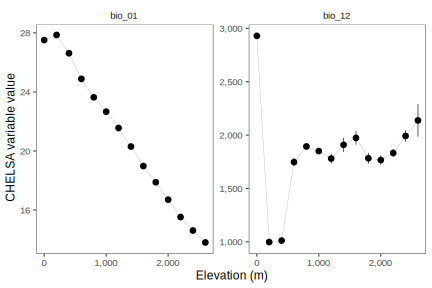
\includegraphics[width=\textwidth]{figs/fig_climate_elev}

\}

\textbackslash{}caption\{CHELSA climatic variables as a function of elevation, in increments of 200m. Points represent means, while vertical lines show 95\% confidence intervals.\}(\#fig:export\_fig\_clim\_elev)
\textbackslash{}end\{figure\}

\hypertarget{landcover-in-relation-to-elevation}{%
\section{Landcover in relation to elevation}\label{landcover-in-relation-to-elevation}}

\hypertarget{get-data-from-landscape-rasters}{%
\subsection{Get data from landscape rasters}\label{get-data-from-landscape-rasters}}

\begin{Shaded}
\begin{Highlighting}[]
\CommentTok{# get data from landscape rasters}
\NormalTok{lc_elev <-}\StringTok{ }\KeywordTok{tibble}\NormalTok{(}\DataTypeTok{elev =} \KeywordTok{getValues}\NormalTok{(landscape[[}\StringTok{"elev"}\NormalTok{]]),}
                  \DataTypeTok{landcover =} \KeywordTok{getValues}\NormalTok{(landscape[[}\StringTok{"landcover"}\NormalTok{]]))}
\CommentTok{# process data for proportions}
\NormalTok{lc_elev <-}\StringTok{ }\NormalTok{lc_elev }\OperatorTok\StringTok{ }
\StringTok{  }\KeywordTok{filter}\NormalTok{(}\OperatorTok{!}\KeywordTok{is.na}\NormalTok{(landcover), landcover }\OperatorTok{!=}\StringTok{ }\DecValTok{0}\NormalTok{) }\OperatorTok\StringTok{ }
\StringTok{  }\KeywordTok{mutate}\NormalTok{(}\DataTypeTok{elev =}\NormalTok{ plyr}\OperatorTok{::}\KeywordTok{round_any}\NormalTok{(elev, }\DecValTok{100}\NormalTok{)) }\OperatorTok\StringTok{ }
\StringTok{  }\KeywordTok{count}\NormalTok{(elev, landcover) }\OperatorTok
\StringTok{  }\KeywordTok{group_by}\NormalTok{(elev) }\OperatorTok\StringTok{ }
\StringTok{  }\KeywordTok{mutate}\NormalTok{(}\DataTypeTok{prop =}\NormalTok{ n}\OperatorTok{/}\KeywordTok{sum}\NormalTok{(n))}
\end{Highlighting}
\end{Shaded}

\hypertarget{plot-proportional-landcover-in-elevation}{%
\subsection{Plot proportional landcover in elevation}\label{plot-proportional-landcover-in-elevation}}

\begin{Shaded}
\begin{Highlighting}[]
\CommentTok{# plot figure as tilemap}
\NormalTok{fig_lc_elev <-}\StringTok{ }\KeywordTok{ggplot}\NormalTok{(lc_elev)}\OperatorTok{+}
\StringTok{  }\KeywordTok{geom_tile}\NormalTok{(}\KeywordTok{aes}\NormalTok{(}\DataTypeTok{x=}\NormalTok{elev, }\DataTypeTok{y=}\KeywordTok{factor}\NormalTok{(landcover), }
                \DataTypeTok{fill=}\NormalTok{prop), }
            \DataTypeTok{col=}\StringTok{"grey99"}\NormalTok{, }\DataTypeTok{size =} \FloatTok{0.6}\NormalTok{)}\OperatorTok{+}
\StringTok{  }\KeywordTok{scale_fill_scico}\NormalTok{(}\DataTypeTok{palette =} \StringTok{"bilbao"}\NormalTok{, }\DataTypeTok{begin =} \FloatTok{0.0}\NormalTok{, }\DataTypeTok{end =} \FloatTok{1.0}\NormalTok{)}\OperatorTok{+}
\StringTok{  }\KeywordTok{scale_x_continuous}\NormalTok{(}\DataTypeTok{breaks =} \KeywordTok{seq}\NormalTok{(}\DecValTok{0}\NormalTok{, }\DecValTok{2500}\NormalTok{, }\DecValTok{500}\NormalTok{), }\DataTypeTok{labels =}\NormalTok{ comma)}\OperatorTok{+}
\StringTok{  }\KeywordTok{scale_alpha_continuous}\NormalTok{(}\DataTypeTok{range =} \KeywordTok{c}\NormalTok{(}\FloatTok{0.3}\NormalTok{, }\DecValTok{1}\NormalTok{))}\OperatorTok{+}
\StringTok{  }\KeywordTok{labs}\NormalTok{(}\DataTypeTok{x =} \StringTok{"elevation (m)"}\NormalTok{, }
       \DataTypeTok{y =} \StringTok{"landcover"}\NormalTok{)}\OperatorTok{+}
\StringTok{  }\KeywordTok{theme_few}\NormalTok{()}

\CommentTok{# export figure}
\KeywordTok{ggsave}\NormalTok{(fig_lc_elev, }\DataTypeTok{filename =} \StringTok{"figs/fig_lc_elev.png"}\NormalTok{, }
       \DataTypeTok{height =} \DecValTok{3}\NormalTok{, }\DataTypeTok{width =} \DecValTok{6}\NormalTok{, }\DataTypeTok{device =} \KeywordTok{png}\NormalTok{(), }\DataTypeTok{dpi =} \DecValTok{300}\NormalTok{); }\KeywordTok{dev.off}\NormalTok{()}
\end{Highlighting}
\end{Shaded}

\begin{Shaded}
\begin{Highlighting}[]

\CommentTok{# show exported image}
\NormalTok{knitr}\OperatorTok{::}\KeywordTok{include_graphics}\NormalTok{(}\StringTok{"figs/fig_lc_elev.png"}\NormalTok{)}
\end{Highlighting}
\end{Shaded}

\textbackslash{}begin\{figure\}

\{\centering \includegraphics[width=\textwidth]{figs/fig_lc_elev}

\}

\caption{Proportional landcover (low = white, high = dark red), as a function of elevation in the study site. Data represent elevation in increments of 100m.}

(\#fig:show\_fig\_lc\_elev)
\textbackslash{}end\{figure\}

\hypertarget{climate-in-relation-to-landcover}{%
\section{Climate in relation to landcover}\label{climate-in-relation-to-landcover}}

\hypertarget{prepare-libraries-3}{%
\subsection{Prepare libraries}\label{prepare-libraries-3}}

\begin{Shaded}
\begin{Highlighting}[]
\CommentTok{# load libs}
\KeywordTok{library}\NormalTok{(raster)}
\KeywordTok{library}\NormalTok{(glue)}
\KeywordTok{library}\NormalTok{(purrr)}
\KeywordTok{library}\NormalTok{(dplyr)}
\KeywordTok{library}\NormalTok{(tidyr)}

\CommentTok{# plotting options}
\KeywordTok{library}\NormalTok{(ggplot2)}
\KeywordTok{library}\NormalTok{(ggthemes)}
\KeywordTok{library}\NormalTok{(scico)}

\CommentTok{# get ci func}
\NormalTok{ci <-}\StringTok{ }\ControlFlowTok{function}\NormalTok{(x)\{}\KeywordTok{qnorm}\NormalTok{(}\FloatTok{0.975}\NormalTok{)}\OperatorTok{*}\KeywordTok{sd}\NormalTok{(x, }\DataTypeTok{na.rm =}\NormalTok{ T)}\OperatorTok{/}\KeywordTok{sqrt}\NormalTok{(}\KeywordTok{length}\NormalTok{(x))\}}
\end{Highlighting}
\end{Shaded}

\begin{Shaded}
\begin{Highlighting}[]
\CommentTok{# read landscape prepare for plotting}
\NormalTok{landscape <-}\StringTok{ }\KeywordTok{stack}\NormalTok{(}\StringTok{"data/spatial/landscape_resamp01km.tif"}\NormalTok{)}

\CommentTok{# get proper names}
\NormalTok{elev_names <-}\StringTok{ }\KeywordTok{c}\NormalTok{(}\StringTok{"elev"}\NormalTok{, }\StringTok{"slope"}\NormalTok{, }\StringTok{"aspect"}\NormalTok{)}
\NormalTok{chelsa_names <-}\StringTok{ }\KeywordTok{c}\NormalTok{(}\StringTok{"chelsa_bio10_04"}\NormalTok{, }\StringTok{"chelsa_bio10_17"}\NormalTok{, }\StringTok{"chelsa_bio10_18"}\NormalTok{,}
                  \StringTok{"chelsa_prec"}\NormalTok{, }\StringTok{"chelsa_temp"}\NormalTok{)}

\KeywordTok{names}\NormalTok{(landscape) <-}\StringTok{ }\KeywordTok{as.character}\NormalTok{(}\KeywordTok{glue}\NormalTok{(}\StringTok{'\{c(elev_names, chelsa_names, "landcover")\}'}\NormalTok{))}
\end{Highlighting}
\end{Shaded}

\begin{Shaded}
\begin{Highlighting}[]
\CommentTok{# make duplicate stack}
\NormalTok{land_data <-}\StringTok{ }\NormalTok{landscape[[}\KeywordTok{c}\NormalTok{(}\StringTok{"landcover"}\NormalTok{, chelsa_names)]]}

\CommentTok{# convert to list}
\NormalTok{land_data <-}\StringTok{ }\KeywordTok{as.list}\NormalTok{(land_data)}

\CommentTok{# map get values over the stack}
\NormalTok{land_data <-}\StringTok{ }\NormalTok{purrr}\OperatorTok{::}\KeywordTok{map}\NormalTok{(land_data, raster}\OperatorTok{::}\NormalTok{getValues)}
\KeywordTok{names}\NormalTok{(land_data) <-}\StringTok{ }\KeywordTok{c}\NormalTok{(}\StringTok{"landcover"}\NormalTok{, chelsa_names)}

\CommentTok{# conver to dataframe and round to 100m}
\NormalTok{land_data <-}\StringTok{ }\KeywordTok{bind_cols}\NormalTok{(land_data)}
\NormalTok{land_data <-}\StringTok{ }\KeywordTok{drop_na}\NormalTok{(land_data) }\OperatorTok\StringTok{ }
\StringTok{  }\KeywordTok{filter}\NormalTok{(landcover }\OperatorTok{!=}\StringTok{ }\DecValTok{0}\NormalTok{) }\OperatorTok\StringTok{ }
\StringTok{  }\KeywordTok{pivot_longer}\NormalTok{(}\DataTypeTok{cols =} \KeywordTok{contains}\NormalTok{(}\StringTok{"chelsa"}\NormalTok{),}
               \DataTypeTok{names_to =} \StringTok{"clim_var"}\NormalTok{) }\CommentTok{#%>% }
\CommentTok{# group_by(landcover, clim_var) %>% }
\CommentTok{# summarise_all(.funs = list(~mean(.), ~ci(.)))}
\end{Highlighting}
\end{Shaded}

\hypertarget{plot-climatic-variables-over-landcover}{%
\subsection{Plot climatic variables over landcover}\label{plot-climatic-variables-over-landcover}}

\begin{Shaded}
\begin{Highlighting}[]
\CommentTok{# plot in facets}

\NormalTok{fig_climate_lc <-}\StringTok{ }\KeywordTok{ggplot}\NormalTok{(land_data)}\OperatorTok{+}
\StringTok{  }\KeywordTok{geom_jitter}\NormalTok{(}\KeywordTok{aes}\NormalTok{(}\DataTypeTok{x =}\NormalTok{ landcover}\FloatTok{-0.25}\NormalTok{, }\DataTypeTok{y=}\NormalTok{value,}
                  \DataTypeTok{col =} \KeywordTok{factor}\NormalTok{(landcover)),}
              \DataTypeTok{width =} \FloatTok{0.2}\NormalTok{,}
              \DataTypeTok{size =} \FloatTok{0.1}\NormalTok{, }\DataTypeTok{alpha =} \FloatTok{0.1}\NormalTok{, }\DataTypeTok{shape =} \DecValTok{4}\NormalTok{)}\OperatorTok{+}
\StringTok{  }\KeywordTok{geom_boxplot}\NormalTok{(}\KeywordTok{aes}\NormalTok{(}\DataTypeTok{x =}\NormalTok{ landcover}\FloatTok{+0.25}\NormalTok{, }\DataTypeTok{y =}\NormalTok{ value, }\DataTypeTok{group =}\NormalTok{ landcover),}
               \DataTypeTok{width =} \FloatTok{0.2}\NormalTok{,}
               \DataTypeTok{outlier.size =} \FloatTok{0.2}\NormalTok{, }\DataTypeTok{alpha =} \FloatTok{0.3}\NormalTok{, }\DataTypeTok{fill =} \OtherTok{NA}\NormalTok{)}\OperatorTok{+}
\StringTok{  }\KeywordTok{scale_colour_scico_d}\NormalTok{(}\DataTypeTok{begin=}\FloatTok{0.2}\NormalTok{, }\DataTypeTok{end=}\FloatTok{0.8}\NormalTok{)}\OperatorTok{+}
\StringTok{  }\KeywordTok{scale_y_continuous}\NormalTok{(}\DataTypeTok{labels =}\NormalTok{ scales}\OperatorTok{::}\NormalTok{comma)}\OperatorTok{+}
\StringTok{  }\KeywordTok{scale_x_continuous}\NormalTok{(}\DataTypeTok{breaks =} \KeywordTok{c}\NormalTok{(}\DecValTok{1}\OperatorTok{:}\DecValTok{7}\NormalTok{))}\OperatorTok{+}
\StringTok{  }\KeywordTok{facet_wrap}\NormalTok{(}\OperatorTok{~}\NormalTok{clim_var, }\DataTypeTok{scales =} \StringTok{"free_y"}\NormalTok{)}\OperatorTok{+}
\StringTok{  }\KeywordTok{theme_few}\NormalTok{()}\OperatorTok{+}
\StringTok{  }\KeywordTok{theme}\NormalTok{(}\DataTypeTok{legend.position =} \StringTok{"none"}\NormalTok{)}\OperatorTok{+}
\StringTok{  }\KeywordTok{labs}\NormalTok{(}\DataTypeTok{x =} \StringTok{"landcover class"}\NormalTok{, }\DataTypeTok{y =} \StringTok{"CHELSA variable value"}\NormalTok{)}

\CommentTok{# save as png}
\KeywordTok{ggsave}\NormalTok{(fig_climate_lc, }\DataTypeTok{filename =} \StringTok{"figs/fig_climate_landcover.png"}\NormalTok{, }
       \DataTypeTok{height =} \DecValTok{5}\NormalTok{, }\DataTypeTok{width =} \DecValTok{8}\NormalTok{, }\DataTypeTok{device =} \KeywordTok{png}\NormalTok{(), }\DataTypeTok{dpi =} \DecValTok{300}\NormalTok{); }\KeywordTok{dev.off}\NormalTok{()}
\end{Highlighting}
\end{Shaded}

\begin{Shaded}
\begin{Highlighting}[]

\CommentTok{# show exported image}
\NormalTok{knitr}\OperatorTok{::}\KeywordTok{include_graphics}\NormalTok{(}\StringTok{"figs/fig_climate_landcover.png"}\NormalTok{)}
\end{Highlighting}
\end{Shaded}

\textbackslash{}begin\{figure\}

\{\centering \includegraphics[width=\textwidth]{figs/fig_climate_landcover}

\}

\caption{CHELSA climatic variables as a function of landcover class. Grey points in the background represent raw data.}

(\#fig:export\_fig\_clim\_lc)
\textbackslash{}end\{figure\}

\hypertarget{obsever-expertise-in-time-and-space}{%
\section{Obsever expertise in time and space}\label{obsever-expertise-in-time-and-space}}

\hypertarget{prepare-libraries-4}{%
\subsection{Prepare libraries}\label{prepare-libraries-4}}

\begin{Shaded}
\begin{Highlighting}[]
\CommentTok{# load libs}
\KeywordTok{library}\NormalTok{(raster)}
\KeywordTok{library}\NormalTok{(glue)}
\KeywordTok{library}\NormalTok{(purrr)}
\KeywordTok{library}\NormalTok{(dplyr)}
\KeywordTok{library}\NormalTok{(tidyr)}
\KeywordTok{library}\NormalTok{(readr)}
\KeywordTok{library}\NormalTok{(scales)}

\CommentTok{# plotting libs}
\KeywordTok{library}\NormalTok{(ggplot2)}
\KeywordTok{library}\NormalTok{(ggthemes)}
\KeywordTok{library}\NormalTok{(scico)}

\CommentTok{# get ci func}
\NormalTok{ci <-}\StringTok{ }\ControlFlowTok{function}\NormalTok{(x)\{}\KeywordTok{qnorm}\NormalTok{(}\FloatTok{0.975}\NormalTok{)}\OperatorTok{*}\KeywordTok{sd}\NormalTok{(x, }\DataTypeTok{na.rm =}\NormalTok{ T)}\OperatorTok{/}\KeywordTok{sqrt}\NormalTok{(}\KeywordTok{length}\NormalTok{(x))\}}
\end{Highlighting}
\end{Shaded}

\begin{Shaded}
\begin{Highlighting}[]
\CommentTok{# read in scores and checklist data and link}
\NormalTok{scores <-}\StringTok{ }\KeywordTok{read_csv}\NormalTok{(}\StringTok{"data/dataObsExpScore.csv"}\NormalTok{)}
\NormalTok{data <-}\StringTok{ }\KeywordTok{read_csv}\NormalTok{(}\StringTok{"data/eBirdChecklistVars.csv"}\NormalTok{)}

\NormalTok{data <-}\StringTok{ }\KeywordTok{left_join}\NormalTok{(data, scores, }\DataTypeTok{by =} \KeywordTok{c}\NormalTok{(}\StringTok{"observer"}\NormalTok{ =}\StringTok{ "observer"}\NormalTok{))}
\NormalTok{data <-}\StringTok{ }\KeywordTok{select}\NormalTok{(data, score, nSp, nSoi, landcover, year) }\OperatorTok\StringTok{ }
\StringTok{  }\KeywordTok{filter}\NormalTok{(}\OperatorTok{!}\KeywordTok{is.na}\NormalTok{(score))}
\end{Highlighting}
\end{Shaded}

\hypertarget{species-seen-in-relation-to-osberver-expertise}{%
\subsection{Species seen in relation to osberver expertise}\label{species-seen-in-relation-to-osberver-expertise}}

\begin{Shaded}
\begin{Highlighting}[]
\CommentTok{# summarise data by rounded score and year}
\NormalTok{data_summary01 <-}\StringTok{ }\NormalTok{data }\OperatorTok\StringTok{ }
\StringTok{  }\KeywordTok{mutate}\NormalTok{(}\DataTypeTok{score =}\NormalTok{ plyr}\OperatorTok{::}\KeywordTok{round_any}\NormalTok{(score, }\FloatTok{0.2}\NormalTok{)) }\OperatorTok\StringTok{ }
\StringTok{  }\KeywordTok{select}\NormalTok{(score, year, nSp, nSoi) }\OperatorTok\StringTok{ }
\StringTok{  }\KeywordTok{pivot_longer}\NormalTok{(}\DataTypeTok{cols =} \KeywordTok{c}\NormalTok{(}\StringTok{"nSp"}\NormalTok{, }\StringTok{"nSoi"}\NormalTok{),}
               \DataTypeTok{names_to =} \StringTok{"variable"}\NormalTok{, }\DataTypeTok{values_to =} \StringTok{"value"}\NormalTok{) }\OperatorTok\StringTok{ }
\StringTok{  }\KeywordTok{group_by}\NormalTok{(score, year, variable) }\OperatorTok\StringTok{ }
\StringTok{  }\KeywordTok{summarise_at}\NormalTok{(}\KeywordTok{vars}\NormalTok{(value), }\KeywordTok{list}\NormalTok{(}\OperatorTok{~}\KeywordTok{mean}\NormalTok{(.), }\OperatorTok{~}\KeywordTok{ci}\NormalTok{(.)))}

\CommentTok{# make plot and export}
\NormalTok{fig_nsp_score <-}\StringTok{ }
\StringTok{  }\KeywordTok{ggplot}\NormalTok{(data_summary01)}\OperatorTok{+}
\StringTok{  }\KeywordTok{geom_jitter}\NormalTok{(}\DataTypeTok{data =}\NormalTok{ data, }\KeywordTok{aes}\NormalTok{(}\DataTypeTok{x =}\NormalTok{ score, }\DataTypeTok{y =}\NormalTok{ nSp), }
             \DataTypeTok{col =} \StringTok{"grey"}\NormalTok{, }\DataTypeTok{alpha =} \FloatTok{0.2}\NormalTok{, }\DataTypeTok{size =} \FloatTok{0.1}\NormalTok{)}\OperatorTok{+}
\StringTok{  }\KeywordTok{geom_pointrange}\NormalTok{(}\KeywordTok{aes}\NormalTok{(}\DataTypeTok{x =}\NormalTok{ score, }\DataTypeTok{y =}\NormalTok{ mean, }
                      \DataTypeTok{ymin=}\NormalTok{mean}\OperatorTok{-}\NormalTok{ci, }\DataTypeTok{ymax=}\NormalTok{mean}\OperatorTok{+}\NormalTok{ci,}
                      \DataTypeTok{col =} \KeywordTok{as.factor}\NormalTok{(variable)),}
                  \DataTypeTok{position =} \KeywordTok{position_dodge}\NormalTok{(}\DataTypeTok{width =} \FloatTok{0.05}\NormalTok{))}\OperatorTok{+}
\StringTok{  }\KeywordTok{facet_wrap}\NormalTok{(}\OperatorTok{~}\NormalTok{year)}\OperatorTok{+}
\StringTok{  }\KeywordTok{scale_y_log10}\NormalTok{()}\OperatorTok{+}
\CommentTok{#  coord_cartesian(ylim=c(0,50))+}
\StringTok{  }\KeywordTok{scale_colour_scico_d}\NormalTok{(}\DataTypeTok{palette =} \StringTok{"cork"}\NormalTok{, }\DataTypeTok{begin =} \FloatTok{0.2}\NormalTok{, }\DataTypeTok{end =} \FloatTok{0.8}\NormalTok{)}\OperatorTok{+}
\StringTok{  }\KeywordTok{labs}\NormalTok{(}\DataTypeTok{x =} \StringTok{"expertise score"}\NormalTok{, }\DataTypeTok{y =} \StringTok{"species reported"}\NormalTok{)}\OperatorTok{+}
\StringTok{  }\KeywordTok{theme_few}\NormalTok{()}\OperatorTok{+}
\StringTok{  }\KeywordTok{theme}\NormalTok{(}\DataTypeTok{legend.position =} \StringTok{"none"}\NormalTok{)}

\CommentTok{# export figure}
\KeywordTok{ggsave}\NormalTok{(}\DataTypeTok{filename =} \StringTok{"figs/fig_nsp_score.png"}\NormalTok{, }\DataTypeTok{width =} \DecValTok{8}\NormalTok{, }\DataTypeTok{height =} \DecValTok{6}\NormalTok{, }\DataTypeTok{device =} \KeywordTok{png}\NormalTok{(), }\DataTypeTok{dpi =} \DecValTok{300}\NormalTok{); }\KeywordTok{dev.off}\NormalTok{()}
\end{Highlighting}
\end{Shaded}

\begin{Shaded}
\begin{Highlighting}[]

\CommentTok{# show exported image}
\NormalTok{knitr}\OperatorTok{::}\KeywordTok{include_graphics}\NormalTok{(}\StringTok{"figs/fig_nsp_score.png"}\NormalTok{)}
\end{Highlighting}
\end{Shaded}

\textbackslash{}begin\{figure\}

\{\centering \includegraphics[width=\textwidth]{figs/fig_nsp_score}

\}

\textbackslash{}caption\{Total number of species (blue) and species of interest to this study (green) reported in checklists from the study area over the years 2013 -- 2018, as a function of the expertise score of the reporting observer. Points represent means, with bars showing the 95\% confidence intervals; data shown are for expertise scores rounded to multiples of 0.2, and the y-axis is on a log scale. Raw data are shown in the background (grey points).\}(\#fig:show\_fig\_nsp\_score)
\textbackslash{}end\{figure\}

\hypertarget{expertise-in-relation-to-landcover}{%
\subsection{Expertise in relation to landcover}\label{expertise-in-relation-to-landcover}}

\begin{Shaded}
\begin{Highlighting}[]
\CommentTok{# plot histograms of expertise scores in different landcover classes}
\NormalTok{data <-}\StringTok{ }\KeywordTok{filter}\NormalTok{(data, }\OperatorTok{!}\KeywordTok{is.na}\NormalTok{(landcover))}

\CommentTok{# make plot}
\NormalTok{fig_exp_lc <-}\StringTok{ }\KeywordTok{ggplot}\NormalTok{(data)}\OperatorTok{+}
\StringTok{  }\KeywordTok{geom_histogram}\NormalTok{(}\KeywordTok{aes}\NormalTok{(}\DataTypeTok{x =}\NormalTok{ score), }\DataTypeTok{fill =} \StringTok{"steelblue"}\NormalTok{, }\DataTypeTok{bins =} \DecValTok{20}\NormalTok{)}\OperatorTok{+}
\StringTok{  }\KeywordTok{facet_wrap}\NormalTok{(}\OperatorTok{~}\NormalTok{landcover, }\DataTypeTok{scales =} \StringTok{"free_y"}\NormalTok{, }\DataTypeTok{labeller =}\NormalTok{ label_both, }\DataTypeTok{nrow =} \DecValTok{2}\NormalTok{)}\OperatorTok{+}
\StringTok{  }\KeywordTok{scale_y_continuous}\NormalTok{(}\DataTypeTok{labels =}\NormalTok{ comma)}\OperatorTok{+}
\StringTok{  }\KeywordTok{theme_few}\NormalTok{()}\OperatorTok{+}
\StringTok{  }\KeywordTok{theme}\NormalTok{(}\DataTypeTok{legend.position =} \StringTok{"none"}\NormalTok{)}\OperatorTok{+}
\StringTok{  }\KeywordTok{labs}\NormalTok{(}\DataTypeTok{x =} \StringTok{"expertise score"}\NormalTok{, }\DataTypeTok{y =} \StringTok{"count"}\NormalTok{)}

\CommentTok{# export figure}

\KeywordTok{ggsave}\NormalTok{(}\DataTypeTok{filename =} \StringTok{"figs/fig_exp_lc.png"}\NormalTok{, }\DataTypeTok{width =} \DecValTok{8}\NormalTok{, }\DataTypeTok{height =} \DecValTok{4}\NormalTok{, }\DataTypeTok{device =} \KeywordTok{png}\NormalTok{(), }\DataTypeTok{dpi =} \DecValTok{300}\NormalTok{); }\KeywordTok{dev.off}\NormalTok{()}
\end{Highlighting}
\end{Shaded}

\begin{Shaded}
\begin{Highlighting}[]

\CommentTok{# show exported image}
\NormalTok{knitr}\OperatorTok{::}\KeywordTok{include_graphics}\NormalTok{(}\StringTok{"figs/fig_exp_lc.png"}\NormalTok{)}
\end{Highlighting}
\end{Shaded}

\textbackslash{}begin\{figure\}

\{\centering \includegraphics[width=\textwidth]{figs/fig_exp_lc}

\}

\caption{Distribution of expertise scores in the seven landcover classes present in the study site.}

(\#fig:show\_fig\_exp\_lc)
\textbackslash{}end\{figure\}

\hypertarget{spatial-autocorrelation-in-climatic-predictors}{%
\section{Spatial autocorrelation in climatic predictors}\label{spatial-autocorrelation-in-climatic-predictors}}

\hypertarget{load-libs-and-prep-data}{%
\subsection{Load libs and prep data}\label{load-libs-and-prep-data}}

\begin{Shaded}
\begin{Highlighting}[]
\CommentTok{# load libs}
\KeywordTok{library}\NormalTok{(raster)}
\KeywordTok{library}\NormalTok{(gstat)}
\KeywordTok{library}\NormalTok{(stars)}
\KeywordTok{library}\NormalTok{(purrr)}
\KeywordTok{library}\NormalTok{(tibble)}
\KeywordTok{library}\NormalTok{(dplyr)}
\KeywordTok{library}\NormalTok{(tidyr)}
\KeywordTok{library}\NormalTok{(glue)}
\KeywordTok{library}\NormalTok{(scales)}
\KeywordTok{library}\NormalTok{(gdalUtils)}

\CommentTok{# plot libs}
\KeywordTok{library}\NormalTok{(ggplot2)}
\KeywordTok{library}\NormalTok{(ggthemes)}
\KeywordTok{library}\NormalTok{(scico)}
\KeywordTok{library}\NormalTok{(gridExtra)}
\KeywordTok{library}\NormalTok{(cowplot)}
\KeywordTok{library}\NormalTok{(ggspatial)}

\CommentTok{#'make custom functiont to convert matrix to df}
\NormalTok{raster_to_df <-}\StringTok{ }\ControlFlowTok{function}\NormalTok{(inp) \{}
  
  \CommentTok{# assert is a raster obj}
\NormalTok{  assertthat}\OperatorTok{::}\KeywordTok{assert_that}\NormalTok{(}\StringTok{"RasterLayer"} \OperatorTok\StringTok{ }\KeywordTok{class}\NormalTok{(inp),}
                          \DataTypeTok{msg =} \StringTok{"input is not a raster"}\NormalTok{)}
  
\NormalTok{  coords <-}\StringTok{ }\KeywordTok{coordinates}\NormalTok{(inp)}
\NormalTok{  vals <-}\StringTok{ }\KeywordTok{getValues}\NormalTok{(inp)}
  
\NormalTok{  data <-}\StringTok{ }\KeywordTok{tibble}\NormalTok{(}\DataTypeTok{x =}\NormalTok{ coords[,}\DecValTok{1}\NormalTok{], }\DataTypeTok{y =}\NormalTok{ coords[,}\DecValTok{2}\NormalTok{], }\DataTypeTok{value =}\NormalTok{ vals)}
  
  \KeywordTok{return}\NormalTok{(data)}
\NormalTok{\}}
\end{Highlighting}
\end{Shaded}

\begin{Shaded}
\begin{Highlighting}[]
\CommentTok{# list landscape covariate stacks}
\NormalTok{landscape_files <-}\StringTok{ "data/spatial/landscape_resamp01km.tif"}
\NormalTok{landscape_data <-}\StringTok{ }\KeywordTok{stack}\NormalTok{(landscape_files)}

\CommentTok{# get proper names}
\NormalTok{\{}
\NormalTok{  elev_names <-}\StringTok{ }\KeywordTok{c}\NormalTok{(}\StringTok{"elev"}\NormalTok{, }\StringTok{"slope"}\NormalTok{, }\StringTok{"aspect"}\NormalTok{)}
\NormalTok{  chelsa_names <-}\StringTok{ }\KeywordTok{c}\NormalTok{(}\StringTok{"chelsa_bio10_04"}\NormalTok{, }\StringTok{"chelsa_bio10_17"}\NormalTok{, }\StringTok{"chelsa_bio10_18"}\NormalTok{,}\StringTok{"chelsa_prec"}\NormalTok{, }\StringTok{"chelsa_temp"}\NormalTok{)}
  \KeywordTok{names}\NormalTok{(landscape_data) <-}\StringTok{ }\KeywordTok{as.character}\NormalTok{(}\KeywordTok{glue}\NormalTok{(}\StringTok{'\{c(elev_names, chelsa_names, "landcover")\}'}\NormalTok{))}
\NormalTok{\}}

\CommentTok{# get chelsa rasters}
\NormalTok{chelsa <-}\StringTok{ }\NormalTok{landscape_data[[chelsa_names]]}
\NormalTok{chelsa <-}\StringTok{ }\NormalTok{purrr}\OperatorTok{::}\KeywordTok{map}\NormalTok{(}\KeywordTok{as.list}\NormalTok{(chelsa), raster_to_df)}
\end{Highlighting}
\end{Shaded}

\hypertarget{calculate-variograms}{%
\subsection{Calculate variograms}\label{calculate-variograms}}

\begin{Shaded}
\begin{Highlighting}[]
\CommentTok{# prep variograms}
\NormalTok{vgrams <-}\StringTok{ }\NormalTok{purrr}\OperatorTok{::}\KeywordTok{map}\NormalTok{(chelsa, }\ControlFlowTok{function}\NormalTok{(z)\{}
\NormalTok{  z <-}\StringTok{ }\KeywordTok{drop_na}\NormalTok{(z)}
\NormalTok{  vgram <-}\StringTok{ }\NormalTok{gstat}\OperatorTok{::}\KeywordTok{variogram}\NormalTok{(value}\OperatorTok{~}\DecValTok{1}\NormalTok{, }\DataTypeTok{loc=}\OperatorTok{~}\NormalTok{x}\OperatorTok{+}\NormalTok{y, }\DataTypeTok{data =}\NormalTok{ z)}
  \KeywordTok{return}\NormalTok{(vgram)}
\NormalTok{\})}

\CommentTok{# save temp}
\KeywordTok{save}\NormalTok{(vgrams, }\DataTypeTok{file =} \StringTok{"data/chelsa/chelsaVariograms.rdata"}\NormalTok{)}

\CommentTok{# get variogram data}
\NormalTok{vgrams <-}\StringTok{ }\NormalTok{purrr}\OperatorTok{::}\KeywordTok{map}\NormalTok{(vgrams, }\ControlFlowTok{function}\NormalTok{(df)\{}
\NormalTok{  df }\OperatorTok\StringTok{ }\KeywordTok{select}\NormalTok{(dist, gamma)}
\NormalTok{\})}
\NormalTok{vgrams <-}\StringTok{ }\KeywordTok{tibble}\NormalTok{(}\DataTypeTok{variable =}\NormalTok{ chelsa_names,}
                 \DataTypeTok{data =}\NormalTok{ vgrams)}
\end{Highlighting}
\end{Shaded}

\begin{Shaded}
\begin{Highlighting}[]
\NormalTok{wg <-}\StringTok{ }\KeywordTok{st_read}\NormalTok{(}\StringTok{"data/spatial/hillsShapefile/Nil_Ana_Pal.shp"}\NormalTok{) }\OperatorTok\StringTok{ }
\StringTok{  }\KeywordTok{st_transform}\NormalTok{(}\DecValTok{32643}\NormalTok{)}
\NormalTok{bbox <-}\StringTok{ }\KeywordTok{st_bbox}\NormalTok{(wg)}

\CommentTok{# add lamd}
\KeywordTok{library}\NormalTok{(rnaturalearth)}
\NormalTok{land <-}\StringTok{ }\KeywordTok{ne_countries}\NormalTok{(}\DataTypeTok{scale =} \DecValTok{50}\NormalTok{, }\DataTypeTok{type =} \StringTok{"countries"}\NormalTok{, }\DataTypeTok{continent =} \StringTok{"asia"}\NormalTok{,}
                     \DataTypeTok{country =} \StringTok{"india"}\NormalTok{,}
                     \DataTypeTok{returnclass =} \KeywordTok{c}\NormalTok{(}\StringTok{"sf"}\NormalTok{))}

\CommentTok{# crop land}
\NormalTok{land <-}\StringTok{ }\KeywordTok{st_transform}\NormalTok{(land, }\DecValTok{32643}\NormalTok{)}
\end{Highlighting}
\end{Shaded}

\hypertarget{plot-chelsa-data-and-variograms}{%
\subsection{Plot CHELSA data and variograms}\label{plot-chelsa-data-and-variograms}}

\begin{Shaded}
\begin{Highlighting}[]
\CommentTok{# make ggplot of variograms}
\NormalTok{yaxis <-}\StringTok{ }\KeywordTok{c}\NormalTok{(}\StringTok{"semivariance"}\NormalTok{, }\KeywordTok{rep}\NormalTok{(}\StringTok{""}\NormalTok{, }\DecValTok{4}\NormalTok{))}
\NormalTok{xaxis <-}\StringTok{ }\KeywordTok{c}\NormalTok{(}\StringTok{""}\NormalTok{, }\StringTok{""}\NormalTok{, }\StringTok{"distance (km)"}\NormalTok{, }\StringTok{""}\NormalTok{, }\StringTok{""}\NormalTok{)}
\NormalTok{fig_vgrams <-}\StringTok{ }\NormalTok{purrr}\OperatorTok{::}\KeywordTok{pmap}\NormalTok{(}\KeywordTok{list}\NormalTok{(vgrams}\OperatorTok{$}\NormalTok{data, yaxis, xaxis), }\ControlFlowTok{function}\NormalTok{(df, ya, xa)\{}
  
  \KeywordTok{ggplot}\NormalTok{(df)}\OperatorTok{+}
\StringTok{    }\KeywordTok{geom_line}\NormalTok{(}\KeywordTok{aes}\NormalTok{(}\DataTypeTok{x =}\NormalTok{ dist}\OperatorTok{/}\DecValTok{1000}\NormalTok{, }\DataTypeTok{y =}\NormalTok{ gamma), }\DataTypeTok{size =} \FloatTok{0.2}\NormalTok{, }\DataTypeTok{col =} \StringTok{"grey"}\NormalTok{)}\OperatorTok{+}
\StringTok{    }\KeywordTok{geom_point}\NormalTok{(}\KeywordTok{aes}\NormalTok{(}\DataTypeTok{x =}\NormalTok{ dist}\OperatorTok{/}\DecValTok{1000}\NormalTok{, }\DataTypeTok{y =}\NormalTok{ gamma), }\DataTypeTok{col =} \StringTok{"black"}\NormalTok{)}\OperatorTok{+}
\StringTok{    }\KeywordTok{scale_x_continuous}\NormalTok{(}\DataTypeTok{labels =}\NormalTok{ comma, }\DataTypeTok{breaks =} \KeywordTok{c}\NormalTok{(}\KeywordTok{seq}\NormalTok{(}\DecValTok{0}\NormalTok{,}\DecValTok{100}\NormalTok{,}\DecValTok{25}\NormalTok{)))}\OperatorTok{+}
\StringTok{    }\KeywordTok{scale_y_log10}\NormalTok{(}\DataTypeTok{labels =}\NormalTok{ comma)}\OperatorTok{+}
\StringTok{    }\KeywordTok{labs}\NormalTok{(}\DataTypeTok{x =}\NormalTok{ xa, }\DataTypeTok{y =}\NormalTok{ ya)}\OperatorTok{+}
\StringTok{    }\KeywordTok{theme_few}\NormalTok{()}\OperatorTok{+}
\StringTok{    }\KeywordTok{theme}\NormalTok{(}\DataTypeTok{axis.text.y =} \KeywordTok{element_text}\NormalTok{(}\DataTypeTok{angle =} \DecValTok{90}\NormalTok{, }\DataTypeTok{hjust =} \FloatTok{0.5}\NormalTok{, }\DataTypeTok{size =} \DecValTok{8}\NormalTok{),}
          \DataTypeTok{strip.text =} \KeywordTok{element_blank}\NormalTok{())}
  
\NormalTok{\})}
\NormalTok{fig_vgrams <-}\StringTok{ }\NormalTok{purrr}\OperatorTok{::}\KeywordTok{map}\NormalTok{(fig_vgrams, as_grob)}

\CommentTok{# make ggplot of chelsa data}
\NormalTok{chelsa <-}\StringTok{ }\KeywordTok{as.list}\NormalTok{(landscape_data[[chelsa_names]]) }\OperatorTok\StringTok{ }
\StringTok{  }\NormalTok{purrr}\OperatorTok{::}\KeywordTok{map}\NormalTok{(st_as_stars)}

\CommentTok{# colour palettes}
\NormalTok{pal <-}\StringTok{ }\KeywordTok{c}\NormalTok{(}\StringTok{"bilbao"}\NormalTok{, }\StringTok{"davos"}\NormalTok{, }\StringTok{"davos"}\NormalTok{, }\StringTok{"nuuk"}\NormalTok{, }\StringTok{"bilbao"}\NormalTok{)}
\NormalTok{title <-}\StringTok{ }\KeywordTok{c}\NormalTok{(}\StringTok{"a Temp. seasonality"}\NormalTok{,}
           \StringTok{"b Ppt. driest qtr."}\NormalTok{,}
           \StringTok{"c Ppt. warmest qtr."}\NormalTok{,}
           \StringTok{"d Variation ppt."}\NormalTok{,}
           \StringTok{"e Variation temp."}\NormalTok{)}
\NormalTok{direction <-}\StringTok{ }\KeywordTok{c}\NormalTok{(}\DecValTok{1}\NormalTok{,}\OperatorTok{-}\DecValTok{1}\NormalTok{,}\OperatorTok{-}\DecValTok{1}\NormalTok{,}\OperatorTok{-}\DecValTok{1}\NormalTok{,}\DecValTok{1}\NormalTok{)}
\NormalTok{lims <-}\StringTok{ }\KeywordTok{list}\NormalTok{(}\KeywordTok{range}\NormalTok{(chelsa[[}\DecValTok{1}\NormalTok{]]}\OperatorTok{$}\NormalTok{chelsa_bio10_}\DecValTok{04}\NormalTok{, }\DataTypeTok{na.rm =}\NormalTok{ T), }
             \KeywordTok{c}\NormalTok{(}\DecValTok{0}\NormalTok{, }\DecValTok{500}\NormalTok{), }\KeywordTok{c}\NormalTok{(}\DecValTok{0}\NormalTok{, }\DecValTok{500}\NormalTok{),}
             \KeywordTok{c}\NormalTok{(}\DecValTok{0}\NormalTok{,}\DecValTok{500}\NormalTok{),}\CommentTok{#range(chelsa[[4]]$chelsa_prec, na.rm = T),}
             \KeywordTok{range}\NormalTok{(chelsa[[}\DecValTok{5}\NormalTok{]]}\OperatorTok{$}\NormalTok{chelsa_temp, }\DataTypeTok{na.rm =}\NormalTok{ T))}
\NormalTok{fig_list_chelsa <-}\StringTok{ }
\StringTok{  }\NormalTok{purrr}\OperatorTok{::}\KeywordTok{pmap}\NormalTok{(}\KeywordTok{list}\NormalTok{(chelsa, pal, title, direction, lims), }
              \ControlFlowTok{function}\NormalTok{(df, pal, t, d, l)\{}
                \KeywordTok{ggplot}\NormalTok{()}\OperatorTok{+}
\StringTok{                  }\KeywordTok{geom_stars}\NormalTok{(}\DataTypeTok{data =}\NormalTok{ df)}\OperatorTok{+}
\StringTok{                  }\KeywordTok{geom_sf}\NormalTok{(}\DataTypeTok{data =}\NormalTok{ land, }\DataTypeTok{fill =} \OtherTok{NA}\NormalTok{, }\DataTypeTok{colour =} \StringTok{"black"}\NormalTok{)}\OperatorTok{+}
\StringTok{                  }\KeywordTok{geom_sf}\NormalTok{(}\DataTypeTok{data =}\NormalTok{ wg, }\DataTypeTok{fill =} \OtherTok{NA}\NormalTok{, }\DataTypeTok{colour =} \StringTok{"black"}\NormalTok{, }\DataTypeTok{size =} \FloatTok{0.3}\NormalTok{)}\OperatorTok{+}
\StringTok{                  }\KeywordTok{scale_fill_scico}\NormalTok{(}\DataTypeTok{palette =}\NormalTok{ pal, }\DataTypeTok{direction =}\NormalTok{ d, }
                                   \DataTypeTok{label =}\NormalTok{ comma, }\DataTypeTok{na.value =} \OtherTok{NA}\NormalTok{, }\DataTypeTok{limits =}\NormalTok{ l)}\OperatorTok{+}
\StringTok{                  }\KeywordTok{coord_sf}\NormalTok{(}\DataTypeTok{xlim =}\NormalTok{ bbox[}\KeywordTok{c}\NormalTok{(}\StringTok{"xmin"}\NormalTok{, }\StringTok{"xmax"}\NormalTok{)], }
                           \DataTypeTok{ylim =}\NormalTok{ bbox[}\KeywordTok{c}\NormalTok{(}\StringTok{"ymin"}\NormalTok{, }\StringTok{"ymax"}\NormalTok{)])}\OperatorTok{+}
\StringTok{                  }\KeywordTok{annotation_scale}\NormalTok{(}\DataTypeTok{location =} \StringTok{"tr"}\NormalTok{, }\DataTypeTok{width_hint =} \FloatTok{0.4}\NormalTok{, }\DataTypeTok{text_cex =} \DecValTok{1}\NormalTok{) }\OperatorTok{+}
\StringTok{                  }
\StringTok{                  }\KeywordTok{theme_few}\NormalTok{()}\OperatorTok{+}
\StringTok{                  }\KeywordTok{theme}\NormalTok{(}\DataTypeTok{legend.position =} \StringTok{"top"}\NormalTok{,}
                        \DataTypeTok{title =} \KeywordTok{element_text}\NormalTok{(}\DataTypeTok{face =} \StringTok{"bold"}\NormalTok{, }\DataTypeTok{size =} \DecValTok{8}\NormalTok{),}
                        \DataTypeTok{legend.key.height =} \KeywordTok{unit}\NormalTok{(}\FloatTok{0.2}\NormalTok{, }\StringTok{"cm"}\NormalTok{),}
                        \DataTypeTok{legend.key.width =} \KeywordTok{unit}\NormalTok{(}\DecValTok{1}\NormalTok{, }\StringTok{"cm"}\NormalTok{),}
                        \DataTypeTok{legend.text =} \KeywordTok{element_text}\NormalTok{(}\DataTypeTok{size =} \DecValTok{8}\NormalTok{),}
                        \DataTypeTok{axis.title =} \KeywordTok{element_blank}\NormalTok{(),}
                        \DataTypeTok{axis.text.y =} \KeywordTok{element_text}\NormalTok{(}\DataTypeTok{angle =} \DecValTok{90}\NormalTok{, }\DataTypeTok{hjust =} \FloatTok{0.5}\NormalTok{),}
                        \CommentTok{# panel.background = element_rect(fill = "lightblue"),}
                        \DataTypeTok{legend.title =} \KeywordTok{element_blank}\NormalTok{())}\OperatorTok{+}
\StringTok{                  }\KeywordTok{labs}\NormalTok{(}\DataTypeTok{x=}\OtherTok{NULL}\NormalTok{, }\DataTypeTok{y=}\OtherTok{NULL}\NormalTok{, }\DataTypeTok{title =}\NormalTok{ t)}
\NormalTok{              \})}
\NormalTok{fig_list_chelsa <-}\StringTok{ }\NormalTok{purrr}\OperatorTok{::}\KeywordTok{map}\NormalTok{(fig_list_chelsa, as_grob)}
\end{Highlighting}
\end{Shaded}

\begin{Shaded}
\begin{Highlighting}[]
\NormalTok{fig_list_chelsa <-}\StringTok{ }\KeywordTok{append}\NormalTok{(fig_list_chelsa, fig_vgrams)}
\NormalTok{lmatrix <-}\StringTok{ }\KeywordTok{matrix}\NormalTok{(}\KeywordTok{c}\NormalTok{(}\KeywordTok{c}\NormalTok{(}\DecValTok{1}\NormalTok{,}\DecValTok{2}\NormalTok{,}\DecValTok{3}\NormalTok{,}\DecValTok{4}\NormalTok{,}\DecValTok{5}\NormalTok{), }\KeywordTok{c}\NormalTok{(}\DecValTok{1}\NormalTok{,}\DecValTok{2}\NormalTok{,}\DecValTok{3}\NormalTok{,}\DecValTok{4}\NormalTok{,}\DecValTok{5}\NormalTok{), }\KeywordTok{c}\NormalTok{(}\DecValTok{6}\NormalTok{,}\DecValTok{7}\NormalTok{,}\DecValTok{8}\NormalTok{,}\DecValTok{9}\NormalTok{,}\DecValTok{10}\NormalTok{)), }\DataTypeTok{nrow =} \DecValTok{3}\NormalTok{, }\DataTypeTok{byrow =}\NormalTok{ T)}
\NormalTok{plot_grid <-}\StringTok{ }\KeywordTok{grid.arrange}\NormalTok{(}\DataTypeTok{grobs =}\NormalTok{ fig_list_chelsa, }\DataTypeTok{layout_matrix =}\NormalTok{ lmatrix)}

\KeywordTok{ggsave}\NormalTok{(}\DataTypeTok{plot =}\NormalTok{ plot_grid, }\DataTypeTok{filename =} \StringTok{"figs/fig_chelsa_variograms.png"}\NormalTok{, }\DataTypeTok{dpi =} \DecValTok{300}\NormalTok{, }\DataTypeTok{width =} \DecValTok{12}\NormalTok{, }\DataTypeTok{height =} \DecValTok{6}\NormalTok{)}
\end{Highlighting}
\end{Shaded}

\begin{Shaded}
\begin{Highlighting}[]

\CommentTok{# show exported image}
\NormalTok{knitr}\OperatorTok{::}\KeywordTok{include_graphics}\NormalTok{(}\StringTok{"figs/fig_chelsa_variograms.png"}\NormalTok{)}
\end{Highlighting}
\end{Shaded}

\textbackslash{}begin\{figure\}

\{\centering \includegraphics[width=\textwidth]{figs/fig_chelsa_variograms}

\}

\caption{CHELSA rasters with study area outline, and associated semivariograms. Semivariograms are on a log-transformed y-axis.}

(\#fig:show\_fig\_chelsa)
\textbackslash{}end\{figure\}

\hypertarget{climatic-raster-resampling}{%
\section{Climatic raster resampling}\label{climatic-raster-resampling}}

\hypertarget{prepare-landcover}{%
\subsection{Prepare landcover}\label{prepare-landcover}}

\begin{Shaded}
\begin{Highlighting}[]
\CommentTok{# read in landcover raster location}
\NormalTok{landcover <-}\StringTok{ "data/landUseClassification/Reprojected Image_26thJan2020_UTM_Ghats.tif"}
\CommentTok{# get extent}
\NormalTok{e =}\StringTok{ }\KeywordTok{bbox}\NormalTok{(}\KeywordTok{raster}\NormalTok{(landcover))}

\CommentTok{# init resolution}
\NormalTok{res_init <-}\StringTok{ }\KeywordTok{res}\NormalTok{(}\KeywordTok{raster}\NormalTok{(landcover))}
\CommentTok{# res to transform to 1000m}
\NormalTok{res_final <-}\StringTok{ }\KeywordTok{map}\NormalTok{(}\KeywordTok{c}\NormalTok{(}\DecValTok{100}\NormalTok{, }\DecValTok{250}\NormalTok{, }\DecValTok{500}\NormalTok{, }\FloatTok{1e3}\NormalTok{, }\FloatTok{2.5e3}\NormalTok{), }\ControlFlowTok{function}\NormalTok{(x)\{x}\OperatorTok{*}\NormalTok{res_init\})}

\CommentTok{# use gdalutils gdalwarp for resampling transform}
\CommentTok{# to 1km from 10m}
\ControlFlowTok{for}\NormalTok{ (i }\ControlFlowTok{in} \DecValTok{1}\OperatorTok{:}\KeywordTok{length}\NormalTok{(res_final)) \{}
\NormalTok{  this_res <-}\StringTok{ }\NormalTok{res_final[[i]]}
\NormalTok{  this_res_char <-}\StringTok{ }\NormalTok{stringr}\OperatorTok{::}\KeywordTok{str_pad}\NormalTok{(this_res[}\DecValTok{1}\NormalTok{], }\DecValTok{5}\NormalTok{, }\DataTypeTok{pad =} \StringTok{"0"}\NormalTok{)}
  \KeywordTok{gdalwarp}\NormalTok{(}\DataTypeTok{srcfile =}\NormalTok{ landcover, }
          \DataTypeTok{dstfile =} \KeywordTok{as.character}\NormalTok{(}\KeywordTok{glue}\NormalTok{(}\StringTok{'data/landUseClassification/lc_\{this_res_char\}m.tif'}\NormalTok{)), }
          \DataTypeTok{tr=}\KeywordTok{c}\NormalTok{(this_res), }\DataTypeTok{r=}\StringTok{'mode'}\NormalTok{, }\DataTypeTok{te=}\KeywordTok{c}\NormalTok{(e))}
\NormalTok{\}}
\end{Highlighting}
\end{Shaded}

\begin{Shaded}
\begin{Highlighting}[]
\CommentTok{# read in resampled landcover raster files as a list}
\NormalTok{lc_files <-}\StringTok{ }\KeywordTok{list.files}\NormalTok{(}\StringTok{"data/landUseClassification/"}\NormalTok{, }\DataTypeTok{pattern =} \StringTok{"lc"}\NormalTok{, }\DataTypeTok{full.names =} \OtherTok{TRUE}\NormalTok{)}
\NormalTok{lc_data <-}\StringTok{ }\KeywordTok{map}\NormalTok{(lc_files, raster)}
\end{Highlighting}
\end{Shaded}

\hypertarget{prepare-spatial-extent}{%
\subsection{Prepare spatial extent}\label{prepare-spatial-extent}}

\begin{Shaded}
\begin{Highlighting}[]
\CommentTok{# load hills}
\KeywordTok{library}\NormalTok{(sf)}
\NormalTok{hills <-}\StringTok{ }\KeywordTok{st_read}\NormalTok{(}\StringTok{"data/spatial/hillsShapefile/Nil_Ana_Pal.shp"}\NormalTok{)}
\NormalTok{hills <-}\StringTok{ }\KeywordTok{st_transform}\NormalTok{(hills, }\DecValTok{32643}\NormalTok{)}
\NormalTok{buffer <-}\StringTok{ }\KeywordTok{st_buffer}\NormalTok{(hills, }\FloatTok{3e4}\NormalTok{) }\OperatorTok\StringTok{ }
\StringTok{  }\KeywordTok{st_transform}\NormalTok{(}\DecValTok{4326}\NormalTok{)}
\NormalTok{bbox <-}\StringTok{ }\KeywordTok{st_bbox}\NormalTok{(hills)}
\end{Highlighting}
\end{Shaded}

\hypertarget{prepare-chelsa-rasters}{%
\subsection{Prepare CHELSA rasters}\label{prepare-chelsa-rasters}}

\begin{Shaded}
\begin{Highlighting}[]
\CommentTok{# list chelsa files}
\NormalTok{chelsaFiles <-}\StringTok{ }\KeywordTok{list.files}\NormalTok{(}\StringTok{"data/chelsa/"}\NormalTok{, }\DataTypeTok{full.names =} \OtherTok{TRUE}\NormalTok{, }\DataTypeTok{pattern =} \StringTok{"*.tif"}\NormalTok{)}

\CommentTok{# gather chelsa rasters}
\NormalTok{chelsaData <-}\StringTok{ }\NormalTok{purrr}\OperatorTok{::}\KeywordTok{map}\NormalTok{(chelsaFiles, }\ControlFlowTok{function}\NormalTok{(chr)\{}
\NormalTok{  a <-}\StringTok{ }\KeywordTok{raster}\NormalTok{(chr)}
  \KeywordTok{crs}\NormalTok{(a) <-}\StringTok{ }\KeywordTok{crs}\NormalTok{(buffer)}
\NormalTok{  a <-}\StringTok{ }\KeywordTok{crop}\NormalTok{(a, }\KeywordTok{as}\NormalTok{(buffer, }\StringTok{"Spatial"}\NormalTok{))}
  \KeywordTok{return}\NormalTok{(a)}
\NormalTok{\})}

\CommentTok{# stack chelsa data}
\NormalTok{chelsaData <-}\StringTok{ }\NormalTok{raster}\OperatorTok{::}\KeywordTok{stack}\NormalTok{(chelsaData)}
\KeywordTok{names}\NormalTok{(chelsaData) <-}\StringTok{ }\KeywordTok{c}\NormalTok{(}\StringTok{"chelsa_bio10_04"}\NormalTok{, }\StringTok{"chelsa_bio10_17"}\NormalTok{, }\StringTok{"chelsa_bio10_18"}\NormalTok{,}\StringTok{"chelsa_prec"}\NormalTok{, }\StringTok{"chelsa_temp"}\NormalTok{)}
\end{Highlighting}
\end{Shaded}

\hypertarget{resample-prepared-rasters}{%
\subsection{Resample prepared rasters}\label{resample-prepared-rasters}}

\begin{Shaded}
\begin{Highlighting}[]
\CommentTok{# make resampled data}
\NormalTok{resamp_data <-}\StringTok{ }\KeywordTok{map}\NormalTok{(lc_data, }\ControlFlowTok{function}\NormalTok{(this_scale)\{}
\NormalTok{  rr <-}\StringTok{ }\KeywordTok{projectRaster}\NormalTok{(}\DataTypeTok{from =}\NormalTok{ chelsaData, }\DataTypeTok{to =}\NormalTok{ this_scale, }
                      \DataTypeTok{crs =} \KeywordTok{crs}\NormalTok{(this_scale), }\DataTypeTok{res =} \KeywordTok{res}\NormalTok{(this_scale))}
\NormalTok{\})}

\CommentTok{# make a stars list}
\NormalTok{resamp_data <-}\StringTok{ }\KeywordTok{map2}\NormalTok{(resamp_data, lc_data, }\ControlFlowTok{function}\NormalTok{(z1,z2)\{}
\NormalTok{  z2[z2 }\OperatorTok{==}\StringTok{ }\DecValTok{0}\NormalTok{] <-}\StringTok{ }\OtherTok{NA}
\NormalTok{  z2 <-}\StringTok{ }\KeywordTok{append}\NormalTok{(z2, }\KeywordTok{as.list}\NormalTok{(z1)) }\OperatorTok\StringTok{ }\KeywordTok{map}\NormalTok{(st_as_stars)}
\NormalTok{\}) }\OperatorTok\StringTok{ }
\StringTok{  }\KeywordTok{flatten}\NormalTok{()}
\end{Highlighting}
\end{Shaded}

\begin{Shaded}
\begin{Highlighting}[]
\CommentTok{# colour palettes}
\NormalTok{pal <-}\StringTok{ }\KeywordTok{c}\NormalTok{(}\StringTok{"batlow"}\NormalTok{, }\StringTok{"bilbao"}\NormalTok{, }\StringTok{"davos"}\NormalTok{, }\StringTok{"davos"}\NormalTok{, }\StringTok{"nuuk"}\NormalTok{, }\StringTok{"bilbao"}\NormalTok{)}
\NormalTok{title <-}\StringTok{ }\KeywordTok{c}\NormalTok{(}\StringTok{"a landcover"}\NormalTok{,}
           \StringTok{"b Temp. seasonality"}\NormalTok{,}
           \StringTok{"c Ppt. driest qtr."}\NormalTok{,}
           \StringTok{"d Ppt. warmest qtr."}\NormalTok{,}
           \StringTok{"e Variation ppt."}\NormalTok{,}
           \StringTok{"f Variation temp."}\NormalTok{)}
\NormalTok{title <-}\StringTok{ }\KeywordTok{c}\NormalTok{(title, }\KeywordTok{rep}\NormalTok{(}\StringTok{""}\NormalTok{, }\DecValTok{24}\NormalTok{))}
\NormalTok{direction <-}\StringTok{ }\KeywordTok{c}\NormalTok{(}\DecValTok{1}\NormalTok{,}\DecValTok{1}\NormalTok{,}\OperatorTok{-}\DecValTok{1}\NormalTok{,}\OperatorTok{-}\DecValTok{1}\NormalTok{,}\OperatorTok{-}\DecValTok{1}\NormalTok{,}\DecValTok{1}\NormalTok{)}

\NormalTok{scales <-}\StringTok{ }\KeywordTok{c}\NormalTok{(}\KeywordTok{c}\NormalTok{(}\StringTok{"1.0km"}\NormalTok{, }\KeywordTok{rep}\NormalTok{(}\StringTok{""}\NormalTok{, }\DecValTok{5}\NormalTok{)), }\KeywordTok{c}\NormalTok{(}\StringTok{"2.5km"}\NormalTok{, }\KeywordTok{rep}\NormalTok{(}\StringTok{""}\NormalTok{, }\DecValTok{5}\NormalTok{)), }
            \KeywordTok{c}\NormalTok{(}\StringTok{"5.0km"}\NormalTok{, }\KeywordTok{rep}\NormalTok{(}\StringTok{""}\NormalTok{, }\DecValTok{5}\NormalTok{)), }\KeywordTok{c}\NormalTok{(}\StringTok{"10km"}\NormalTok{, }\KeywordTok{rep}\NormalTok{(}\StringTok{""}\NormalTok{, }\DecValTok{5}\NormalTok{)), }
            \KeywordTok{c}\NormalTok{(}\StringTok{"25km"}\NormalTok{, }\KeywordTok{rep}\NormalTok{(}\StringTok{""}\NormalTok{, }\DecValTok{5}\NormalTok{)))}

\CommentTok{# make figures across the list}
\NormalTok{fig_list_chelsa_resamp <-}\StringTok{ }
\StringTok{  }\NormalTok{purrr}\OperatorTok{::}\KeywordTok{pmap}\NormalTok{(}\KeywordTok{list}\NormalTok{(resamp_data, scales, }\KeywordTok{rep}\NormalTok{(pal, }\DecValTok{5}\NormalTok{), title, }\KeywordTok{rep}\NormalTok{(direction, }\DecValTok{5}\NormalTok{)), }
              \ControlFlowTok{function}\NormalTok{(df, scale, pal, t, d)\{}
                \KeywordTok{ggplot}\NormalTok{()}\OperatorTok{+}
\StringTok{                  }\KeywordTok{geom_stars}\NormalTok{(}\DataTypeTok{data =}\NormalTok{ df)}\OperatorTok{+}
\StringTok{                  }\KeywordTok{geom_sf}\NormalTok{(}\DataTypeTok{data =}\NormalTok{ hills, }\DataTypeTok{fill =} \OtherTok{NA}\NormalTok{, }\DataTypeTok{colour =} \StringTok{"black"}\NormalTok{, }\DataTypeTok{size =} \FloatTok{0.3}\NormalTok{)}\OperatorTok{+}
\StringTok{                  }\KeywordTok{scale_fill_scico}\NormalTok{(}\DataTypeTok{palette =}\NormalTok{ pal, }\DataTypeTok{direction =}\NormalTok{ d,}
                                   \DataTypeTok{label =}\NormalTok{ comma, }\DataTypeTok{na.value =} \OtherTok{NA}\NormalTok{)}\OperatorTok{+}
\StringTok{                  }\KeywordTok{coord_sf}\NormalTok{(}\DataTypeTok{xlim =}\NormalTok{ bbox[}\KeywordTok{c}\NormalTok{(}\StringTok{"xmin"}\NormalTok{, }\StringTok{"xmax"}\NormalTok{)],}
                           \DataTypeTok{ylim =}\NormalTok{ bbox[}\KeywordTok{c}\NormalTok{(}\StringTok{"ymin"}\NormalTok{, }\StringTok{"ymax"}\NormalTok{)])}\OperatorTok{+}
\StringTok{                  }\KeywordTok{theme_void}\NormalTok{()}\OperatorTok{+}
\StringTok{                  }\KeywordTok{theme}\NormalTok{(}\CommentTok{#legend.position = "top",}
                    \DataTypeTok{panel.border =} \KeywordTok{element_rect}\NormalTok{(),}
                        \DataTypeTok{title =} \KeywordTok{element_text}\NormalTok{(}\DataTypeTok{face =} \StringTok{"bold"}\NormalTok{, }\DataTypeTok{size =} \DecValTok{8}\NormalTok{),}
                        \CommentTok{# legend.key.height = unit(0.1, "cm"),}
                        \CommentTok{# legend.key.width = unit(0.6, "cm"),}
                        \CommentTok{# legend.text = element_text(size = 8),}
                        \DataTypeTok{axis.title =} \KeywordTok{element_text}\NormalTok{(),}
                        \DataTypeTok{axis.title.y =} \KeywordTok{element_text}\NormalTok{(}\DataTypeTok{angle =} \DecValTok{90}\NormalTok{),}
                        \CommentTok{# axis.text.y = element_text(angle = 90, hjust = 0.5),}
                        \CommentTok{# panel.background = element_rect(fill = "lightblue"),}
                        \DataTypeTok{legend.title =} \KeywordTok{element_blank}\NormalTok{())}\OperatorTok{+}
\StringTok{                  }\KeywordTok{labs}\NormalTok{(}\DataTypeTok{x=}\OtherTok{NULL}\NormalTok{, }\DataTypeTok{y=}\NormalTok{scale, }\DataTypeTok{title =}\NormalTok{ t)}
\NormalTok{              \})}
\NormalTok{fig_list_chelsa_resamp <-}\StringTok{ }\NormalTok{purrr}\OperatorTok{::}\KeywordTok{map}\NormalTok{(fig_list_chelsa_resamp, as_grob)}

\NormalTok{fig_chelsa_resamp <-}\StringTok{ }\KeywordTok{grid.arrange}\NormalTok{(}\DataTypeTok{grobs =}\NormalTok{ fig_list_chelsa_resamp, }\DataTypeTok{ncol=}\DecValTok{6}\NormalTok{)}
\KeywordTok{ggsave}\NormalTok{(}\DataTypeTok{plot =}\NormalTok{ fig_chelsa_resamp, }\DataTypeTok{filename =} \StringTok{"figs/fig_chelsa_resamp.png"}\NormalTok{, }\DataTypeTok{dpi =} \DecValTok{100}\NormalTok{, }\DataTypeTok{width =} \DecValTok{24}\NormalTok{, }\DataTypeTok{height =} \DecValTok{12}\NormalTok{, }\DataTypeTok{device =} \KeywordTok{png}\NormalTok{(), }\DataTypeTok{units =} \StringTok{"in"}\NormalTok{)}

\CommentTok{# use magick to convert}
\KeywordTok{library}\NormalTok{(magick)}
\NormalTok{pl <-}\StringTok{ }\KeywordTok{image_read_pdf}\NormalTok{(}\StringTok{"figs/fig_chelsa_resamp.pdf"}\NormalTok{)}
\KeywordTok{image_write}\NormalTok{(pl, }\DataTypeTok{path =} \StringTok{"figs/fig_chelsa_resamp.png"}\NormalTok{, }\DataTypeTok{format =} \StringTok{"png"}\NormalTok{)}
\end{Highlighting}
\end{Shaded}

\begin{Shaded}
\begin{Highlighting}[]

\CommentTok{# show exported image}
\NormalTok{knitr}\OperatorTok{::}\KeywordTok{include_graphics}\NormalTok{(}\StringTok{"figs/fig_chelsa_resamp.png"}\NormalTok{)}
\end{Highlighting}
\end{Shaded}

\textbackslash{}begin\{figure\}

\{\centering \includegraphics[width=\textwidth]{figs/fig_chelsa_resamp}

\}

\caption{CHELSA rasters with study area outline, at different scales. Semivariograms are on a log-transformed y-axis.}

(\#fig:show\_fig\_chelsa\_resamp)
\textbackslash{}end\{figure\}

\hypertarget{matching-effort-with-spatial-independence}{%
\section{Matching effort with spatial independence}\label{matching-effort-with-spatial-independence}}

How many sites would be lost if effort distance was restricted based on spatial independence?

\hypertarget{load-librarires}{%
\subsection{Load librarires}\label{load-librarires}}

\begin{Shaded}
\begin{Highlighting}[]
\CommentTok{# load data packagaes}
\KeywordTok{library}\NormalTok{(data.table)}
\KeywordTok{library}\NormalTok{(dplyr)}

\CommentTok{# load plotting packages}
\KeywordTok{library}\NormalTok{(ggplot2)}
\KeywordTok{library}\NormalTok{(scico)}
\KeywordTok{library}\NormalTok{(ggthemes)}
\KeywordTok{library}\NormalTok{(scales)}
\end{Highlighting}
\end{Shaded}

\hypertarget{load-data}{%
\subsection{Load data}\label{load-data}}

\begin{Shaded}
\begin{Highlighting}[]
\CommentTok{# load checklist covariates}
\NormalTok{data <-}\StringTok{ }\KeywordTok{fread}\NormalTok{(}\StringTok{"data/eBirdChecklistVars.csv"}\NormalTok{)}

\NormalTok{effort_distance_summary <-}\StringTok{ }\NormalTok{data[, effort_distance_class }\OperatorTok{:}\ErrorTok{=}\StringTok{ }\KeywordTok{cut}\NormalTok{(distance, }\DataTypeTok{breaks =} \KeywordTok{c}\NormalTok{(}\OperatorTok{-}\DecValTok{1}\NormalTok{, }\FloatTok{0.001}\NormalTok{, }\FloatTok{0.1}\NormalTok{, }\FloatTok{0.25}\NormalTok{, }\FloatTok{0.5}\NormalTok{, }\DecValTok{1}\NormalTok{, }\FloatTok{2.5}\NormalTok{, }\DecValTok{5}\NormalTok{, }\OtherTok{Inf}\NormalTok{), }\DataTypeTok{ordered_result =}\NormalTok{ T)}
\NormalTok{     ][,.N, by =}\StringTok{ }\NormalTok{effort_distance_class}
\NormalTok{       ][}\KeywordTok{order}\NormalTok{(effort_distance_class)]}

\NormalTok{effort_distance_summary[,prop_effort}\OperatorTok{:}\ErrorTok{=}\KeywordTok{cumsum}\NormalTok{(effort_distance_summary}\OperatorTok{$}\NormalTok{N)}\OperatorTok{/}\KeywordTok{nrow}\NormalTok{(data)]}
\end{Highlighting}
\end{Shaded}

\hypertarget{plot-distance-exclusion-effect}{%
\subsection{Plot distance exclusion effect}\label{plot-distance-exclusion-effect}}

\begin{Shaded}
\begin{Highlighting}[]
\CommentTok{# plot effort distance class cumulative sum}
\NormalTok{fig_dist_exclusion <-}\StringTok{ }\KeywordTok{ggplot}\NormalTok{(effort_distance_summary)}\OperatorTok{+}
\StringTok{  }\KeywordTok{geom_point}\NormalTok{(}\KeywordTok{aes}\NormalTok{(effort_distance_class, prop_effort), }\DataTypeTok{size =} \DecValTok{3}\NormalTok{)}\OperatorTok{+}
\StringTok{  }\KeywordTok{geom_path}\NormalTok{(}\KeywordTok{aes}\NormalTok{(effort_distance_class, prop_effort, }\DataTypeTok{group =} \OtherTok{NA}\NormalTok{))}\OperatorTok{+}
\StringTok{  }\CommentTok{# scale_y_continuous(label=label_number(scale=0.001, accuracy = 1, suffix = "K"))+}
\StringTok{  }\KeywordTok{scale_x_discrete}\NormalTok{(}\DataTypeTok{labels =} \KeywordTok{c}\NormalTok{(}\StringTok{"stationary"}\NormalTok{, }\StringTok{"100m"}\NormalTok{, }\StringTok{"250m"}\NormalTok{, }\StringTok{"500m"}\NormalTok{, }\StringTok{"1 km"}\NormalTok{, }\StringTok{"2.5 km"}\NormalTok{, }\StringTok{"5 km"}\NormalTok{))}\OperatorTok{+}
\StringTok{  }\KeywordTok{theme_few}\NormalTok{()}\OperatorTok{+}
\StringTok{  }\KeywordTok{theme}\NormalTok{(}\DataTypeTok{panel.grid =} \KeywordTok{element_line}\NormalTok{(}\DataTypeTok{size =} \FloatTok{0.2}\NormalTok{, }\DataTypeTok{color =} \StringTok{"grey"}\NormalTok{))}\OperatorTok{+}
\StringTok{  }\KeywordTok{labs}\NormalTok{(}\DataTypeTok{x =} \StringTok{"effort distance cutoff"}\NormalTok{, }\DataTypeTok{y =} \StringTok{"proportion of checklists"}\NormalTok{)}

\KeywordTok{ggsave}\NormalTok{(}\DataTypeTok{plot =}\NormalTok{ fig_dist_exclusion, }\StringTok{"figs/fig_cutoff_effort.png"}\NormalTok{, }\DataTypeTok{height =} \DecValTok{6}\NormalTok{, }\DataTypeTok{width =} \DecValTok{8}\NormalTok{, }\DataTypeTok{dpi =} \DecValTok{300}\NormalTok{)}
\KeywordTok{dev.off}\NormalTok{()}
\end{Highlighting}
\end{Shaded}

\begin{Shaded}
\begin{Highlighting}[]
\NormalTok{knitr}\OperatorTok{::}\KeywordTok{include_graphics}\NormalTok{(}\StringTok{"figs/fig_cutoff_effort.png"}\NormalTok{)}
\end{Highlighting}
\end{Shaded}

\begin{center}\includegraphics[width=\textwidth]{figs/fig_cutoff_effort} \end{center}

\hypertarget{spatial-thinning-a-comparison-of-approaches}{%
\section{Spatial thinning: A comparison of approaches}\label{spatial-thinning-a-comparison-of-approaches}}

\hypertarget{prepare-libraries-5}{%
\subsection{Prepare libraries}\label{prepare-libraries-5}}

\begin{Shaded}
\begin{Highlighting}[]
\CommentTok{# load libraries}
\KeywordTok{library}\NormalTok{(tidyverse)}
\KeywordTok{library}\NormalTok{(glue)}
\KeywordTok{library}\NormalTok{(readr)}
\KeywordTok{library}\NormalTok{(sf)}

\CommentTok{# plotting}
\KeywordTok{library}\NormalTok{(ggthemes)}
\KeywordTok{library}\NormalTok{(scico)}
\KeywordTok{library}\NormalTok{(scales)}

\CommentTok{# ci func}
\NormalTok{ci <-}\StringTok{ }\ControlFlowTok{function}\NormalTok{(x)\{}\KeywordTok{qnorm}\NormalTok{(}\FloatTok{0.975}\NormalTok{)}\OperatorTok{*}\KeywordTok{sd}\NormalTok{(x, }\DataTypeTok{na.rm =}\NormalTok{ T)}\OperatorTok{/}\KeywordTok{sqrt}\NormalTok{(}\KeywordTok{length}\NormalTok{(x))\}}

\CommentTok{# load python libs here}
\KeywordTok{library}\NormalTok{(reticulate)}
\CommentTok{# set python path}
\KeywordTok{use_python}\NormalTok{(}\StringTok{"/usr/bin/python3"}\NormalTok{)}
\end{Highlighting}
\end{Shaded}

\hypertarget{traditional-grid-based-thinning}{%
\subsection{Traditional grid-based thinning}\label{traditional-grid-based-thinning}}

\begin{Shaded}
\begin{Highlighting}[]
\CommentTok{# load the shapefile of the study area}
\NormalTok{wg <-}\StringTok{ }\KeywordTok{st_read}\NormalTok{(}\StringTok{"data/spatial/hillsShapefile/Nil_Ana_Pal.shp"}\NormalTok{) }\OperatorTok\StringTok{ }
\StringTok{  }\KeywordTok{st_transform}\NormalTok{(}\DecValTok{32643}\NormalTok{)}

\CommentTok{# get scales}
\CommentTok{# load checklist data and select one per rounded 500m coordinates}
\NormalTok{\{}
\NormalTok{  data <-}\StringTok{ }\KeywordTok{read_csv}\NormalTok{(}\StringTok{"data/eBirdChecklistVars.csv"}\NormalTok{) }\OperatorTok\StringTok{ }
\StringTok{    }\KeywordTok{count}\NormalTok{(longitude, latitude, }\DataTypeTok{name =} \StringTok{"tot_effort"}\NormalTok{)}
    
  
  \CommentTok{# how many unique points}
\NormalTok{  n_all_points <-}\StringTok{ }\KeywordTok{nrow}\NormalTok{(data)}
\NormalTok{  d_all_effort <-}\StringTok{ }\KeywordTok{sum}\NormalTok{(data}\OperatorTok{$}\NormalTok{tot_effort)}
  
  \CommentTok{# round to different scales}
\NormalTok{  scale <-}\StringTok{ }\KeywordTok{c}\NormalTok{(}\DecValTok{100}\NormalTok{, }\DecValTok{250}\NormalTok{, }\DecValTok{500}\NormalTok{, }\DecValTok{1000}\NormalTok{)}
  
  \CommentTok{# group data by scale}
\NormalTok{  data <-}\StringTok{ }\KeywordTok{crossing}\NormalTok{(scale, data) }\OperatorTok\StringTok{ }
\StringTok{    }\KeywordTok{group_by}\NormalTok{(scale) }\OperatorTok\StringTok{ }
\StringTok{    }\KeywordTok{nest}\NormalTok{() }\OperatorTok\StringTok{ }
\StringTok{    }\KeywordTok{ungroup}\NormalTok{()}
\NormalTok{\}}

\CommentTok{# select one point per grid cell}
\NormalTok{data <-}\StringTok{ }\KeywordTok{mutate}\NormalTok{(data, }\DataTypeTok{data =} \KeywordTok{map2}\NormalTok{(scale, data, }\ControlFlowTok{function}\NormalTok{(sc, df)\{}
  \CommentTok{# transform the data}
\NormalTok{  df <-}\StringTok{ }\NormalTok{df }\OperatorTok\StringTok{ }
\StringTok{    }\KeywordTok{st_as_sf}\NormalTok{(}\DataTypeTok{coords =} \KeywordTok{c}\NormalTok{(}\StringTok{"longitude"}\NormalTok{, }\StringTok{"latitude"}\NormalTok{)) }\OperatorTok\StringTok{ }
\StringTok{    `}\DataTypeTok{st_crs<-}\StringTok{`}\NormalTok{(}\DecValTok{4326}\NormalTok{) }\OperatorTok\StringTok{ }
\StringTok{    }\KeywordTok{st_transform}\NormalTok{(}\DecValTok{32643}\NormalTok{) }\OperatorTok\StringTok{ }
\StringTok{    }\KeywordTok{bind_cols}\NormalTok{(}\KeywordTok{as_tibble}\NormalTok{(}\KeywordTok{st_coordinates}\NormalTok{(.))) }\OperatorTok\StringTok{ }
\StringTok{    }\KeywordTok{mutate}\NormalTok{(}\DataTypeTok{coordId =} \DecValTok{1}\OperatorTok{:}\KeywordTok{nrow}\NormalTok{(.),}
           \DataTypeTok{X_round =}\NormalTok{ plyr}\OperatorTok{::}\KeywordTok{round_any}\NormalTok{(X, sc),}
           \DataTypeTok{Y_round =}\NormalTok{ plyr}\OperatorTok{::}\KeywordTok{round_any}\NormalTok{(Y, sc))}
  
  \CommentTok{# make a grid}
\NormalTok{  grid <-}\StringTok{ }\KeywordTok{st_make_grid}\NormalTok{(wg, }\DataTypeTok{cellsize =}\NormalTok{ sc)}
  
  \CommentTok{# which cell contains which points}
\NormalTok{  grid_contents <-}\StringTok{ }\KeywordTok{st_contains}\NormalTok{(grid, df) }\OperatorTok\StringTok{ }
\StringTok{    }\KeywordTok{as_tibble}\NormalTok{() }\OperatorTok\StringTok{ }
\StringTok{    }\KeywordTok{rename}\NormalTok{(}\DataTypeTok{cell =}\NormalTok{ row.id, }\DataTypeTok{coordId =}\NormalTok{ col.id)}
  
  \KeywordTok{rm}\NormalTok{(grid)}
  
  \CommentTok{# what's the max point in each grid}
\NormalTok{  points_max <-}\StringTok{ }\KeywordTok{left_join}\NormalTok{(df }\OperatorTok\StringTok{ }\KeywordTok{st_drop_geometry}\NormalTok{(),}
\NormalTok{                   grid_contents, }\DataTypeTok{by =} \StringTok{"coordId"}\NormalTok{) }\OperatorTok\StringTok{ }
\StringTok{    }\KeywordTok{group_by}\NormalTok{(cell) }\OperatorTok\StringTok{ }
\StringTok{    }\KeywordTok{filter}\NormalTok{(tot_effort }\OperatorTok{==}\StringTok{ }\KeywordTok{max}\NormalTok{(tot_effort))}
  
  \CommentTok{# get summary for max}
\NormalTok{  max_sites <-}\StringTok{ }\NormalTok{points_max }\OperatorTok\StringTok{ }
\StringTok{    }\KeywordTok{ungroup}\NormalTok{() }\OperatorTok\StringTok{ }
\StringTok{    }\KeywordTok{summarise}\NormalTok{(}\DataTypeTok{prop_points=} \KeywordTok{length}\NormalTok{(coordId)}\OperatorTok{/}\NormalTok{n_all_points,}
              \DataTypeTok{prop_effort =} \KeywordTok{sum}\NormalTok{(tot_effort)}\OperatorTok{/}\NormalTok{d_all_effort) }\OperatorTok\StringTok{ }
\StringTok{    }\KeywordTok{pivot_longer}\NormalTok{(}\DataTypeTok{cols =} \KeywordTok{everything}\NormalTok{(),}
                 \DataTypeTok{names_to =} \StringTok{"variable"}\NormalTok{)}
  
  \CommentTok{# select a random point in each grid}
\NormalTok{  points_rand <-}\StringTok{ }\KeywordTok{left_join}\NormalTok{(df }\OperatorTok\StringTok{ }\KeywordTok{st_drop_geometry}\NormalTok{(),}
\NormalTok{                   grid_contents, }\DataTypeTok{by =} \StringTok{"coordId"}\NormalTok{) }\OperatorTok\StringTok{ }
\StringTok{    }\KeywordTok{group_by}\NormalTok{(cell) }\OperatorTok\StringTok{ }
\StringTok{    }\KeywordTok{sample_n}\NormalTok{(}\DataTypeTok{size =} \DecValTok{1}\NormalTok{)}
  
  \CommentTok{# get summary for rand}
\NormalTok{  rand_sites <-}\StringTok{ }\NormalTok{points_rand }\OperatorTok\StringTok{ }
\StringTok{    }\KeywordTok{ungroup}\NormalTok{() }\OperatorTok\StringTok{ }
\StringTok{    }\KeywordTok{summarise}\NormalTok{(}\DataTypeTok{prop_points =} \KeywordTok{length}\NormalTok{(coordId)}\OperatorTok{/}\NormalTok{n_all_points,}
              \DataTypeTok{prop_effort =} \KeywordTok{sum}\NormalTok{(tot_effort)}\OperatorTok{/}\NormalTok{d_all_effort) }\OperatorTok\StringTok{ }
\StringTok{    }\KeywordTok{pivot_longer}\NormalTok{(}\DataTypeTok{cols =} \KeywordTok{everything}\NormalTok{(),}
                 \DataTypeTok{names_to =} \StringTok{"variable"}\NormalTok{)}
  
\NormalTok{  df <-}\StringTok{ }\KeywordTok{tibble}\NormalTok{(}\DataTypeTok{grid_rand =} \KeywordTok{list}\NormalTok{(rand_sites), }\DataTypeTok{grid_max =} \KeywordTok{list}\NormalTok{(max_sites),}
               \DataTypeTok{points_rand =} \KeywordTok{list}\NormalTok{(points_rand), }\DataTypeTok{points_max =} \KeywordTok{list}\NormalTok{(points_max))}
\NormalTok{\}))}

\CommentTok{# unnest data}
\NormalTok{data <-}\StringTok{ }\KeywordTok{unnest}\NormalTok{(data, }\DataTypeTok{cols =}\NormalTok{ data)}

\CommentTok{# save summary as another object}
\NormalTok{data_thin_trad <-}\StringTok{ }\NormalTok{data }\OperatorTok\StringTok{ }
\StringTok{  }\KeywordTok{select}\NormalTok{(}\OperatorTok{-}\KeywordTok{contains}\NormalTok{(}\StringTok{"points"}\NormalTok{)) }\OperatorTok\StringTok{ }
\StringTok{  }\KeywordTok{pivot_longer}\NormalTok{(}\DataTypeTok{cols =} \OperatorTok{-}\KeywordTok{contains}\NormalTok{(}\StringTok{"scale"}\NormalTok{),}
               \DataTypeTok{names_to =} \StringTok{"method"}\NormalTok{, }\DataTypeTok{values_to =} \StringTok{"somedata"}\NormalTok{) }\OperatorTok\StringTok{ }
\StringTok{  }\KeywordTok{unnest}\NormalTok{(}\DataTypeTok{cols =}\NormalTok{ somedata)}

\CommentTok{# save points for later comparison}
\NormalTok{points_thin_trad <-}\StringTok{ }\NormalTok{data }\OperatorTok\StringTok{ }
\StringTok{  }\KeywordTok{select}\NormalTok{(}\KeywordTok{contains}\NormalTok{(}\StringTok{"points"}\NormalTok{), scale)}

\KeywordTok{rm}\NormalTok{(data)}
\end{Highlighting}
\end{Shaded}

\hypertarget{network-based-thinning}{%
\subsection{Network-based thinning}\label{network-based-thinning}}

Load python libraries.

\begin{Shaded}
\begin{Highlighting}[]
\CommentTok{# import classic python libs}
\ImportTok{import}\NormalTok{ numpy }\ImportTok{as}\NormalTok{ np}
\ImportTok{import}\NormalTok{ matplotlib.pyplot }\ImportTok{as}\NormalTok{ plt}

\CommentTok{# libs for dataframes}
\ImportTok{import}\NormalTok{ pandas }\ImportTok{as}\NormalTok{ pd}

\CommentTok{# network lib}
\ImportTok{import}\NormalTok{ networkx }\ImportTok{as}\NormalTok{ nx}

\CommentTok{# import libs for geodata}
\ImportTok{import}\NormalTok{ geopandas }\ImportTok{as}\NormalTok{ gpd}

\CommentTok{# import ckdtree}
\ImportTok{from}\NormalTok{ scipy.spatial }\ImportTok{import}\NormalTok{ cKDTree}
\end{Highlighting}
\end{Shaded}

\hypertarget{finding-modularity-in-proximity-networks}{%
\subsection{Finding modularity in proximity networks}\label{finding-modularity-in-proximity-networks}}

\begin{Shaded}
\begin{Highlighting}[]
\CommentTok{# read in checklist covariates for conversion to gpd}
\CommentTok{# get unique coordinates, assign them to the df}
\CommentTok{# convert df to geo-df}
\NormalTok{chkCovars }\OperatorTok{=}\NormalTok{ pd.read_csv(}\StringTok{"data/eBirdChecklistVars.csv"}\NormalTok{)}
\NormalTok{ul }\OperatorTok{=}\NormalTok{ chkCovars[[}\StringTok{'longitude'}\NormalTok{, }\StringTok{'latitude'}\NormalTok{]].drop_duplicates(subset}\OperatorTok{=}\NormalTok{[}\StringTok{'longitude'}\NormalTok{, }\StringTok{'latitude'}\NormalTok{])}
\NormalTok{ul[}\StringTok{'coordId'}\NormalTok{] }\OperatorTok{=}\NormalTok{ np.arange(}\DecValTok{0}\NormalTok{, ul.shape[}\DecValTok{0}\NormalTok{])}

\CommentTok{# get effort at each coordinate}
\NormalTok{effort }\OperatorTok{=}\NormalTok{ chkCovars.groupby([}\StringTok{'longitude'}\NormalTok{, }\StringTok{'latitude'}\NormalTok{]).size().to_frame(}\StringTok{'tot_effort'}\NormalTok{)}
\NormalTok{effort }\OperatorTok{=}\NormalTok{ effort.reset_index()}

\CommentTok{# merge effort on ul}
\NormalTok{ul }\OperatorTok{=}\NormalTok{ pd.merge(ul, effort, on}\OperatorTok{=}\NormalTok{[}\StringTok{'longitude'}\NormalTok{, }\StringTok{'latitude'}\NormalTok{])}

\CommentTok{# make gpd and drop col from ul}
\NormalTok{ulgpd }\OperatorTok{=}\NormalTok{ gpd.GeoDataFrame(ul, geometry}\OperatorTok{=}\NormalTok{gpd.points_from_xy(ul.longitude, ul.latitude))}
\NormalTok{ulgpd.crs }\OperatorTok{=}\NormalTok{ \{}\StringTok{'init'}\NormalTok{ :}\StringTok{'epsg:4326'}\NormalTok{\}}
\CommentTok{# reproject spatials to 43n epsg 32643}
\NormalTok{ulgpd }\OperatorTok{=}\NormalTok{ ulgpd.to_crs(\{}\StringTok{'init'}\NormalTok{: }\StringTok{'epsg:32643'}\NormalTok{\})}
\NormalTok{ul }\OperatorTok{=}\NormalTok{ pd.DataFrame(ul.drop(columns}\OperatorTok{=}\StringTok{"geometry"}\NormalTok{))}

\CommentTok{# function to use ckdtrees for nearest point finding}
\KeywordTok{def}\NormalTok{ ckd_pairs(gdfA, dist_indep):}
\NormalTok{    A }\OperatorTok{=}\NormalTok{ np.concatenate([np.array(geom.coords) }\ControlFlowTok{for}\NormalTok{ geom }\KeywordTok{in}\NormalTok{ gdfA.geometry.to_list()])}
\NormalTok{    ckd_tree }\OperatorTok{=}\NormalTok{ cKDTree(A)}
\NormalTok{    dist }\OperatorTok{=}\NormalTok{ ckd_tree.query_pairs(r}\OperatorTok{=}\NormalTok{dist_indep, output_type}\OperatorTok{=}\StringTok{'ndarray'}\NormalTok{)}
    \ControlFlowTok{return}\NormalTok{ dist}

\CommentTok{# define scales in metres}
\NormalTok{scales }\OperatorTok{=}\NormalTok{ [}\DecValTok{100}\NormalTok{, }\DecValTok{250}\NormalTok{, }\DecValTok{500}\NormalTok{, }\DecValTok{1000}\NormalTok{]}


\CommentTok{# function to process ckd_pairs}
\KeywordTok{def}\NormalTok{ make_modules(scale):}
\NormalTok{    site_pairs }\OperatorTok{=}\NormalTok{ ckd_pairs(gdfA}\OperatorTok{=}\NormalTok{ulgpd, dist_indep}\OperatorTok{=}\NormalTok{scale)}
\NormalTok{    site_pairs }\OperatorTok{=}\NormalTok{ pd.DataFrame(data}\OperatorTok{=}\NormalTok{site_pairs, columns}\OperatorTok{=}\NormalTok{[}\StringTok{'p1'}\NormalTok{, }\StringTok{'p2'}\NormalTok{])}
\NormalTok{    site_pairs[}\StringTok{'scale'}\NormalTok{] }\OperatorTok{=}\NormalTok{ scale}
    \CommentTok{# get site ids}
\NormalTok{    site_id }\OperatorTok{=}\NormalTok{ np.concatenate((site_pairs.p1.unique(), site_pairs.p2.unique()))}
\NormalTok{    site_id }\OperatorTok{=}\NormalTok{ np.unique(site_id)}
    \CommentTok{# make network}
\NormalTok{    network }\OperatorTok{=}\NormalTok{ nx.from_pandas_edgelist(site_pairs, }\StringTok{'p1'}\NormalTok{, }\StringTok{'p2'}\NormalTok{)}
    \CommentTok{# get modules}
\NormalTok{    modules }\OperatorTok{=} \BuiltInTok{list}\NormalTok{(nx.algorithms.community.greedy_modularity_communities(network))}
    \CommentTok{# get modules as df}
\NormalTok{    m }\OperatorTok{=}\NormalTok{ []}
    \ControlFlowTok{for}\NormalTok{ i }\KeywordTok{in}\NormalTok{ np.arange(}\BuiltInTok{len}\NormalTok{(modules)):}
\NormalTok{        module_number }\OperatorTok{=}\NormalTok{ [i] }\OperatorTok{*} \BuiltInTok{len}\NormalTok{(modules[i])}
\NormalTok{        module_coords }\OperatorTok{=} \BuiltInTok{list}\NormalTok{(modules[i])}
\NormalTok{        m }\OperatorTok{=}\NormalTok{ m }\OperatorTok{+} \BuiltInTok{list}\NormalTok{(}\BuiltInTok{zip}\NormalTok{(module_number, module_coords))}
    \CommentTok{# add location and summed sampling duration}
\NormalTok{    unique_locs }\OperatorTok{=}\NormalTok{ ul[ul.coordId.isin(site_id)]}
\NormalTok{    module_data }\OperatorTok{=}\NormalTok{ pd.DataFrame(m, columns}\OperatorTok{=}\NormalTok{[}\StringTok{'module'}\NormalTok{, }\StringTok{'coordId'}\NormalTok{])}
\NormalTok{    module_data }\OperatorTok{=}\NormalTok{ pd.merge(module_data, unique_locs, on}\OperatorTok{=}\StringTok{'coordId'}\NormalTok{)}
    \CommentTok{# add scale}
\NormalTok{    module_data[}\StringTok{'scale'}\NormalTok{] }\OperatorTok{=}\NormalTok{ scale}
    \ControlFlowTok{return}\NormalTok{ [site_pairs, module_data]}


\CommentTok{# run make modules on ulgpd at scales}
\NormalTok{data }\OperatorTok{=} \BuiltInTok{list}\NormalTok{(}\BuiltInTok{map}\NormalTok{(make_modules, scales))}

\CommentTok{# extract data for output}
\NormalTok{tot_pair_data }\OperatorTok{=}\NormalTok{ []}
\NormalTok{tot_module_data }\OperatorTok{=}\NormalTok{ []}
\ControlFlowTok{for}\NormalTok{ i }\KeywordTok{in}\NormalTok{ np.arange(}\BuiltInTok{len}\NormalTok{(data)):}
\NormalTok{    tot_pair_data.append(data[i][}\DecValTok{0}\NormalTok{])}
\NormalTok{    tot_module_data.append(data[i][}\DecValTok{1}\NormalTok{])}

\NormalTok{tot_pair_data }\OperatorTok{=}\NormalTok{ pd.concat(tot_pair_data, ignore_index}\OperatorTok{=}\VariableTok{True}\NormalTok{)}
\NormalTok{tot_module_data }\OperatorTok{=}\NormalTok{ pd.concat(tot_module_data, ignore_index}\OperatorTok{=}\VariableTok{True}\NormalTok{)}

\CommentTok{# make dict of positions and array of coordinates}
\CommentTok{# site_id = np.concatenate((site_pairs.p1.unique(), site_pairs.p2.unique()))}
\CommentTok{# site_id = np.unique(site_id)}
\CommentTok{# locations_df = ul[ul.coordId.isin(site_id)][['longitude', 'latitude']].to_numpy()}
\CommentTok{# pos_dict = dict(zip(site_id, locations_df))}

\CommentTok{# output data}
\NormalTok{tot_module_data.to_csv(path_or_buf}\OperatorTok{=}\StringTok{"data/site_modules.csv"}\NormalTok{, index}\OperatorTok{=}\VariableTok{False}\NormalTok{)}
\NormalTok{tot_pair_data.to_csv(path_or_buf}\OperatorTok{=}\StringTok{"data/site_pairs.csv"}\NormalTok{, index}\OperatorTok{=}\VariableTok{False}\NormalTok{)}

\CommentTok{# ends here}
\end{Highlighting}
\end{Shaded}

\hypertarget{process-proximity-networks-in-r}{%
\subsection{Process proximity networks in R}\label{process-proximity-networks-in-r}}

\begin{Shaded}
\begin{Highlighting}[]
\CommentTok{# read in pair and module data}
\NormalTok{pairs <-}\StringTok{ }\KeywordTok{read_csv}\NormalTok{(}\StringTok{"data/site_pairs.csv"}\NormalTok{)}
\NormalTok{mods <-}\StringTok{ }\KeywordTok{read_csv}\NormalTok{(}\StringTok{"data/site_modules.csv"}\NormalTok{)}

\CommentTok{# count pairs at each scale}
\KeywordTok{count}\NormalTok{(pairs, scale)}
\NormalTok{pairs }\OperatorTok\StringTok{ }
\StringTok{  }\KeywordTok{group_by}\NormalTok{(scale) }\OperatorTok\StringTok{ }
\StringTok{  }\KeywordTok{summarise}\NormalTok{(}\DataTypeTok{non_indep_pairs =} \KeywordTok{length}\NormalTok{(}\KeywordTok{unique}\NormalTok{(}\KeywordTok{c}\NormalTok{(p1, p2)))}\OperatorTok{/}\NormalTok{n_all_points)}
\KeywordTok{count}\NormalTok{(mods, scale)}

\CommentTok{# nest by scale and add module data}
\NormalTok{data <-}\StringTok{ }\KeywordTok{nest}\NormalTok{(pairs, }\DataTypeTok{data =} \KeywordTok{c}\NormalTok{(p1, p2))}
\NormalTok{modules <-}\StringTok{ }\KeywordTok{group_by}\NormalTok{(mods, scale) }\OperatorTok\StringTok{ }
\StringTok{  }\KeywordTok{nest}\NormalTok{() }\OperatorTok\StringTok{ }\KeywordTok{ungroup}\NormalTok{()}

\CommentTok{# add module data}
\NormalTok{data <-}\StringTok{ }\KeywordTok{mutate}\NormalTok{(data, }
               \DataTypeTok{modules =}\NormalTok{ modules}\OperatorTok{$}\NormalTok{data,}
               \DataTypeTok{data =} \KeywordTok{map2}\NormalTok{(data, modules, }\ControlFlowTok{function}\NormalTok{(df, m)\{}
\NormalTok{                 df <-}\StringTok{ }\KeywordTok{left_join}\NormalTok{(df, m, }\DataTypeTok{by =} \KeywordTok{c}\NormalTok{(}\StringTok{"p1"}\NormalTok{ =}\StringTok{ "coordId"}\NormalTok{))}
\NormalTok{                 df <-}\StringTok{ }\KeywordTok{left_join}\NormalTok{(df, m, }\DataTypeTok{by =} \KeywordTok{c}\NormalTok{(}\StringTok{"p2"}\NormalTok{ =}\StringTok{ "coordId"}\NormalTok{))}
                 
\NormalTok{                 df <-}\StringTok{ }\KeywordTok{filter}\NormalTok{(df, module.x }\OperatorTok{==}\StringTok{ }\NormalTok{module.y)  }
                 \KeywordTok{return}\NormalTok{(df)}
\NormalTok{               \})) }\OperatorTok\StringTok{ }
\StringTok{  }\KeywordTok{select}\NormalTok{(}\OperatorTok{-}\NormalTok{modules)}

\CommentTok{# split by module}
\NormalTok{data}\OperatorTok{$}\NormalTok{data <-}\StringTok{ }\KeywordTok{map}\NormalTok{(data}\OperatorTok{$}\NormalTok{data, }\ControlFlowTok{function}\NormalTok{(df)\{}
\NormalTok{  df <-}\StringTok{ }\KeywordTok{group_by}\NormalTok{(df, module.x, module.y) }\OperatorTok\StringTok{ }
\StringTok{    }\KeywordTok{nest}\NormalTok{() }\OperatorTok\StringTok{ }
\StringTok{    }\KeywordTok{ungroup}\NormalTok{()}
  \KeywordTok{return}\NormalTok{(df)}
\NormalTok{\})}
\end{Highlighting}
\end{Shaded}

\hypertarget{a-function-that-removes-sites}{%
\subsection{A function that removes sites}\label{a-function-that-removes-sites}}

\begin{Shaded}
\begin{Highlighting}[]

\CommentTok{# a function to remove sites}
\NormalTok{remove_which_sites <-}\StringTok{ }\ControlFlowTok{function}\NormalTok{(pair_data)\{}
  
\NormalTok{  \{}
\NormalTok{    a =}\StringTok{ }\NormalTok{pair_data }\OperatorTok\StringTok{  }
\StringTok{      }\KeywordTok{select}\NormalTok{(p1, p2)}
    
\NormalTok{    nodes_a_init =}\StringTok{ }\KeywordTok{unique}\NormalTok{(}\KeywordTok{c}\NormalTok{(a}\OperatorTok{$}\NormalTok{p1, a}\OperatorTok{$}\NormalTok{p2))}
    
\NormalTok{    i_n_d =}\StringTok{ }\KeywordTok{filter}\NormalTok{(mods, coordId }\OperatorTok\StringTok{ }\NormalTok{nodes_a_init) }\OperatorTok\StringTok{ }
\StringTok{      }\KeywordTok{select}\NormalTok{(}\DataTypeTok{node =}\NormalTok{ coordId, tot_effort) }\OperatorTok\StringTok{ }
\StringTok{      }\KeywordTok{mutate}\NormalTok{(}\DataTypeTok{s_f_r =} \OtherTok{NA}\NormalTok{)}
    
\NormalTok{    nodes_keep =}\StringTok{ }\KeywordTok{c}\NormalTok{()}
\NormalTok{    nodes_removed =}\StringTok{ }\KeywordTok{c}\NormalTok{()}
\NormalTok{  \}}
  
  \ControlFlowTok{while}\NormalTok{(}\KeywordTok{nrow}\NormalTok{(a) }\OperatorTok{>}\StringTok{ }\DecValTok{0}\NormalTok{)\{}
    
    \CommentTok{# how many nodes in a}
\NormalTok{    nodes_a =}\StringTok{ }\KeywordTok{unique}\NormalTok{(}\KeywordTok{c}\NormalTok{(a}\OperatorTok{$}\NormalTok{p1, a}\OperatorTok{$}\NormalTok{p2))}
    
    \CommentTok{# get node or site efforts and arrange in ascending order}
\NormalTok{    b =}\StringTok{ }\NormalTok{i_n_d }\OperatorTok\StringTok{ }\KeywordTok{filter}\NormalTok{(node }\OperatorTok\StringTok{ }\NormalTok{nodes_a)}
    
    \ControlFlowTok{for}\NormalTok{ (i }\ControlFlowTok{in} \DecValTok{1}\OperatorTok{:}\KeywordTok{nrow}\NormalTok{(b))\{}
      \CommentTok{# which node to remove}
\NormalTok{      node_out =}\StringTok{ }\NormalTok{b}\OperatorTok{$}\NormalTok{node[i]}
      \CommentTok{# how much tot_effort lost}
\NormalTok{      d_n_o =}\StringTok{ }\NormalTok{b}\OperatorTok{$}\NormalTok{tot_effort[i]}
      
      \CommentTok{# how many rows remain in a if node_out is removed?}
\NormalTok{      a_n_o =}\StringTok{ }\KeywordTok{filter}\NormalTok{(a, p1 }\OperatorTok{!=}\StringTok{ }\NormalTok{node_out, p2 }\OperatorTok{!=}\StringTok{ }\NormalTok{node_out)}
\NormalTok{      indep_nodes =}\StringTok{ }\KeywordTok{setdiff}\NormalTok{(nodes_a, }\KeywordTok{unique}\NormalTok{(}\KeywordTok{c}\NormalTok{(a_n_o}\OperatorTok{$}\NormalTok{p1, a_n_o}\OperatorTok{$}\NormalTok{p2, node_out)))}
      
      \CommentTok{# how much sampling effort made spatially independent}
\NormalTok{      indep_sampling =}\StringTok{ }\KeywordTok{filter}\NormalTok{(b, node }\OperatorTok\StringTok{ }\NormalTok{indep_nodes) }\OperatorTok\StringTok{ }
\StringTok{        }\KeywordTok{summarise}\NormalTok{(}\DataTypeTok{tot_effort =} \KeywordTok{sum}\NormalTok{(tot_effort)) }\OperatorTok\StringTok{ }
\StringTok{        }\NormalTok{.}\OperatorTok{$}\NormalTok{tot_effort}
      
      \CommentTok{# message(glue::glue('\{node_out\} removal frees \{indep_sampling\} m'))}
      \CommentTok{# sampling freed by sampling lost}
\NormalTok{      b}\OperatorTok{$}\NormalTok{s_f_r[i] =}\StringTok{ }\NormalTok{indep_sampling}\OperatorTok{/}\NormalTok{d_n_o}
\NormalTok{    \}}
    
    \CommentTok{# arrange node data by decreasing sfr and increasing tot_effort}
    \CommentTok{# highest tot_effort nodes are processed last}
\NormalTok{    b =}\StringTok{ }\KeywordTok{arrange}\NormalTok{(b, }\OperatorTok{-}\NormalTok{s_f_r, tot_effort)}
    
\NormalTok{    nodes_removed =}\StringTok{ }\KeywordTok{c}\NormalTok{(nodes_removed, b}\OperatorTok{$}\NormalTok{node[}\DecValTok{1}\NormalTok{])}
    
    \CommentTok{# remove pairs of nodes containing the highest sfr node in b}
\NormalTok{    a =}\StringTok{ }\KeywordTok{filter}\NormalTok{(a, p1 }\OperatorTok{!=}\StringTok{ }\NormalTok{b}\OperatorTok{$}\NormalTok{node[}\DecValTok{1}\NormalTok{], p2 }\OperatorTok{!=}\StringTok{ }\NormalTok{b}\OperatorTok{$}\NormalTok{node[}\DecValTok{1}\NormalTok{])}
    
\NormalTok{    nodes_keep =}\StringTok{ }\KeywordTok{c}\NormalTok{(nodes_keep, }\KeywordTok{setdiff}\NormalTok{(nodes_a, }\KeywordTok{unique}\NormalTok{(}\KeywordTok{c}\NormalTok{(a}\OperatorTok{$}\NormalTok{p1, a}\OperatorTok{$}\NormalTok{p2, nodes_removed))))}
    
\NormalTok{  \}}
  
  \KeywordTok{message}\NormalTok{(glue}\OperatorTok{::}\KeywordTok{glue}\NormalTok{(}\StringTok{'keeping \{length(nodes_keep)\} of \{length(nodes_a_init)\}'}\NormalTok{))}
  
  \CommentTok{# node_status <- tibble(nodes = c(nodes_keep, nodes_removed),}
  \CommentTok{#                       status = c(rep(TRUE, length(nodes_keep)),}
  \CommentTok{#                                  rep(FALSE, length(nodes_removed))))}
  
  \KeywordTok{return}\NormalTok{(}\KeywordTok{as.integer}\NormalTok{(nodes_removed))}
\NormalTok{\}}
\end{Highlighting}
\end{Shaded}

\hypertarget{removing-non-independent-sites}{%
\subsection{Removing non-independent sites}\label{removing-non-independent-sites}}

\begin{Shaded}
\begin{Highlighting}[]
\CommentTok{# remove 5km and 2.5km scale}
\NormalTok{data <-}\StringTok{ }\NormalTok{data }\OperatorTok\StringTok{ }\KeywordTok{filter}\NormalTok{(scale }\OperatorTok{<=}\DecValTok{1000}\NormalTok{)}
\CommentTok{# run select sites on the various modules}
\NormalTok{sites_removed <-}\StringTok{ }\KeywordTok{map}\NormalTok{(data}\OperatorTok{$}\NormalTok{data, }\ControlFlowTok{function}\NormalTok{(df)\{}
\NormalTok{  remove_sites <-}\StringTok{ }\KeywordTok{unlist}\NormalTok{(purrr}\OperatorTok{::}\KeywordTok{map}\NormalTok{(df}\OperatorTok{$}\NormalTok{data, remove_which_sites))}
\NormalTok{\})}

\CommentTok{# save as rdata}
\KeywordTok{save}\NormalTok{(sites_removed, }\DataTypeTok{file =} \StringTok{"data/data_network_sites_removed.rdata"}\NormalTok{)}
\end{Highlighting}
\end{Shaded}

\begin{Shaded}
\begin{Highlighting}[]
\CommentTok{# get python sites}
\NormalTok{ul =}\StringTok{ }\NormalTok{py}\OperatorTok{$}\NormalTok{ul}

\KeywordTok{load}\NormalTok{(}\StringTok{"data/data_network_sites_removed.rdata"}\NormalTok{)}

\CommentTok{# subset sites}
\NormalTok{data <-}\StringTok{ }\KeywordTok{mutate}\NormalTok{(data,}
               \DataTypeTok{data =} \KeywordTok{map}\NormalTok{(sites_removed, }\ControlFlowTok{function}\NormalTok{(site_id)\{}
                 \KeywordTok{as_tibble}\NormalTok{(}\KeywordTok{filter}\NormalTok{(ul, }\OperatorTok{!}\NormalTok{coordId }\OperatorTok\StringTok{ }\NormalTok{site_id))}
\NormalTok{               \}))}

\CommentTok{# which points are kept}
\NormalTok{points_thin_net <-}\StringTok{ }\KeywordTok{mutate}\NormalTok{(data,}
                          \DataTypeTok{data =} \KeywordTok{map}\NormalTok{(data,}\ControlFlowTok{function}\NormalTok{(df)\{}
\NormalTok{                            df <-}\StringTok{ }\NormalTok{df }\OperatorTok\StringTok{ }
\StringTok{                              }\KeywordTok{select}\NormalTok{(}\StringTok{"longitude"}\NormalTok{, }\StringTok{"latitude"}\NormalTok{) }\OperatorTok\StringTok{ }
\StringTok{                              }\KeywordTok{st_as_sf}\NormalTok{(}\DataTypeTok{coords =} \KeywordTok{c}\NormalTok{(}\StringTok{"longitude"}\NormalTok{, }\StringTok{"latitude"}\NormalTok{)) }\OperatorTok\StringTok{ }
\StringTok{                              `}\DataTypeTok{st_crs<-}\StringTok{`}\NormalTok{(}\DecValTok{4326}\NormalTok{) }\OperatorTok\StringTok{ }
\StringTok{                              }\KeywordTok{st_transform}\NormalTok{(}\DecValTok{32643}\NormalTok{) }\OperatorTok\StringTok{ }
\StringTok{                              }\KeywordTok{bind_cols}\NormalTok{(}\KeywordTok{as_tibble}\NormalTok{(}\KeywordTok{st_coordinates}\NormalTok{(.))) }\OperatorTok\StringTok{ }
\StringTok{                              }\KeywordTok{st_drop_geometry}\NormalTok{()}
\NormalTok{                          \}))}

\CommentTok{# get metrics for method}
\NormalTok{data_thin_net <-}\StringTok{ }\KeywordTok{unnest}\NormalTok{(data, }\DataTypeTok{cols =} \StringTok{"data"}\NormalTok{) }\OperatorTok\StringTok{ }
\StringTok{  }\KeywordTok{group_by}\NormalTok{(scale) }\OperatorTok\StringTok{ }
\StringTok{  }\KeywordTok{summarise}\NormalTok{(}\DataTypeTok{prop_points =} \KeywordTok{length}\NormalTok{(coordId)}\OperatorTok{/}\NormalTok{n_all_points,}
            \DataTypeTok{prop_effort =} \KeywordTok{sum}\NormalTok{(tot_effort)}\OperatorTok{/}\NormalTok{d_all_effort) }\OperatorTok\StringTok{ }
\StringTok{  }\KeywordTok{mutate}\NormalTok{(}\DataTypeTok{method =} \StringTok{"network"}\NormalTok{) }\OperatorTok\StringTok{ }
\StringTok{  }\KeywordTok{pivot_longer}\NormalTok{(}\DataTypeTok{cols =} \OperatorTok{-}\KeywordTok{one_of}\NormalTok{(}\KeywordTok{c}\NormalTok{(}\StringTok{"method"}\NormalTok{, }\StringTok{"scale"}\NormalTok{)),}
               \DataTypeTok{names_to =} \StringTok{"variable"}\NormalTok{)}
\end{Highlighting}
\end{Shaded}

\hypertarget{measuring-method-fallibility}{%
\subsection{Measuring method fallibility}\label{measuring-method-fallibility}}

How many points, at different spatial scales, remain after the application of each method?

\hypertarget{prepare-data-for-python}{%
\subsection{Prepare data for Python}\label{prepare-data-for-python}}

\begin{Shaded}
\begin{Highlighting}[]

\CommentTok{# get points by each method}
\NormalTok{points_list <-}\StringTok{ }\KeywordTok{append}\NormalTok{(points_thin_net}\OperatorTok{$}\NormalTok{data, }\DataTypeTok{values =} \KeywordTok{append}\NormalTok{(points_thin_trad}\OperatorTok{$}\NormalTok{points_rand,}
\NormalTok{                                                            points_thin_trad}\OperatorTok{$}\NormalTok{points_max))}

\CommentTok{# get scales as list}
\NormalTok{scales_list <-}\StringTok{ }\KeywordTok{list}\NormalTok{(}\DecValTok{100}\NormalTok{,}\DecValTok{250}\NormalTok{,}\DecValTok{500}\NormalTok{,}\DecValTok{1000}\NormalTok{, }\KeywordTok{rep}\NormalTok{(}\KeywordTok{c}\NormalTok{(}\DecValTok{100}\NormalTok{,}\DecValTok{250}\NormalTok{, }\DecValTok{500}\NormalTok{,}\DecValTok{1000}\NormalTok{), }\DecValTok{2}\NormalTok{)) }\OperatorTok\StringTok{ }\KeywordTok{flatten}\NormalTok{()}

\CommentTok{# send to python}
\NormalTok{py}\OperatorTok{$}\NormalTok{points_list =}\StringTok{ }\NormalTok{points_list}
\NormalTok{py}\OperatorTok{$}\NormalTok{scales_list =}\StringTok{ }\NormalTok{scales_list}
\end{Highlighting}
\end{Shaded}

\hypertarget{count-props-under-threshold-in-python}{%
\subsection{Count props under threshold in Python}\label{count-props-under-threshold-in-python}}

\begin{Shaded}
\begin{Highlighting}[]
\CommentTok{# transform each element to gpd}


\CommentTok{# a function to convert to gpd}
\KeywordTok{def}\NormalTok{ make_gpd(df):}
\NormalTok{    df }\OperatorTok{=}\NormalTok{ gpd.GeoDataFrame(df, geometry}\OperatorTok{=}\NormalTok{gpd.points_from_xy(df.X, df.Y))}
\NormalTok{    df.crs }\OperatorTok{=}\NormalTok{ \{}\StringTok{'init'}\NormalTok{ :}\StringTok{'epsg:32643'}\NormalTok{\}}
    \ControlFlowTok{return}\NormalTok{ df}


\CommentTok{# function for mean nnd}
\CommentTok{# function to use ckdtrees for nearest point finding}
\KeywordTok{def}\NormalTok{ ckd_test(gdfA, gdfB, dist_indep):}
\NormalTok{    A }\OperatorTok{=}\NormalTok{ np.concatenate([np.array(geom.coords) }\ControlFlowTok{for}\NormalTok{ geom }\KeywordTok{in}\NormalTok{ gdfA.geometry.to_list()])}
    \CommentTok{#simplified_features = simplify_roads(gdfB)}
\NormalTok{    B }\OperatorTok{=}\NormalTok{ np.concatenate([np.array(geom.coords) }\ControlFlowTok{for}\NormalTok{ geom }\KeywordTok{in}\NormalTok{ gdfB.geometry.to_list()])}
    \CommentTok{#B = np.concatenate(B)}
\NormalTok{    ckd_tree }\OperatorTok{=}\NormalTok{ cKDTree(B)}
\NormalTok{    dist, idx }\OperatorTok{=}\NormalTok{ ckd_tree.query(A, k}\OperatorTok{=}\NormalTok{[}\DecValTok{2}\NormalTok{])}
\NormalTok{    dist_diff }\OperatorTok{=} \BuiltInTok{list}\NormalTok{(}\BuiltInTok{map}\NormalTok{(}\KeywordTok{lambda}\NormalTok{ x: x }\OperatorTok{-}\NormalTok{ dist_indep, dist))}
\NormalTok{    mean_dist_diff }\OperatorTok{=}\NormalTok{ np.asarray(dist_diff).mean()}
    \ControlFlowTok{return}\NormalTok{ mean_dist_diff}


\CommentTok{# apply to all data}
\NormalTok{points_list }\OperatorTok{=} \BuiltInTok{list}\NormalTok{(}\BuiltInTok{map}\NormalTok{(make_gpd, points_list))}

\CommentTok{# get nnb all data}
\NormalTok{mean_dist_diff }\OperatorTok{=} \BuiltInTok{list}\NormalTok{(}\BuiltInTok{map}\NormalTok{(ckd_test, points_list, points_list, scales_list))}

\CommentTok{# count points above threshold}
\CommentTok{# n_non_indep = []}
\CommentTok{# for i in np.arange(len(points_list)):}
\CommentTok{#     ni_pairs = ckd_test(gdfA=points_list[i],gdfB=points_list[i], dist_indep=scales_list[i])}
\CommentTok{#     ni_pairs = pd.DataFrame(data=ni_pairs, columns=['p1', 'p2'])}
\CommentTok{#     site_id = np.concatenate((ni_pairs.p1.unique(), ni_pairs.p2.unique()))}
\CommentTok{#     ni_sites = len(np.unique(site_id))/points_list[i].shape[0]}
\CommentTok{#     n_non_indep.append(ni_sites)}
\end{Highlighting}
\end{Shaded}

\hypertarget{plot-metrics-for-different-methods}{%
\subsection{Plot metrics for different methods}\label{plot-metrics-for-different-methods}}

\begin{Shaded}
\begin{Highlighting}[]
\CommentTok{# combine the thinning metrics data}
\NormalTok{data_plot <-}\StringTok{ }\KeywordTok{bind_rows}\NormalTok{(data_thin_net, data_thin_trad)}

\CommentTok{# get data for mean distance}
\NormalTok{data_thin_compare <-}\StringTok{ }\KeywordTok{tibble}\NormalTok{(}\DataTypeTok{scale =} \KeywordTok{unlist}\NormalTok{(scales_list),}
                            \DataTypeTok{method =} \KeywordTok{c}\NormalTok{(}\KeywordTok{rep}\NormalTok{(}\StringTok{"network"}\NormalTok{, }\DecValTok{4}\NormalTok{),}
                                       \KeywordTok{rep}\NormalTok{(}\StringTok{"grid_rand"}\NormalTok{, }\DecValTok{4}\NormalTok{),}
                                       \KeywordTok{rep}\NormalTok{(}\StringTok{"grid_max"}\NormalTok{, }\DecValTok{4}\NormalTok{)),}
                            \StringTok{`}\DataTypeTok{mean NND - buffer (m)}\StringTok{`}\NormalTok{ =}\StringTok{ }\KeywordTok{unlist}\NormalTok{(py}\OperatorTok{$}\NormalTok{mean_dist_diff)) }\OperatorTok\StringTok{ }
\StringTok{  }\KeywordTok{pivot_longer}\NormalTok{(}\DataTypeTok{cols =} \StringTok{"mean NND - buffer (m)"}\NormalTok{,}
               \DataTypeTok{names_to =} \StringTok{"variable"}\NormalTok{)}

\CommentTok{# bind rows with other data}
\NormalTok{data_plot <-}\StringTok{ }\KeywordTok{bind_rows}\NormalTok{(data_plot, data_thin_compare)}

\CommentTok{# plot results}
\NormalTok{fig_spatial_thinning <-}
\StringTok{  }\KeywordTok{ggplot}\NormalTok{(data_plot)}\OperatorTok{+}
\StringTok{  }\KeywordTok{geom_vline}\NormalTok{(}\DataTypeTok{xintercept =}\NormalTok{ scale, }\DataTypeTok{lty =} \DecValTok{3}\NormalTok{, }\DataTypeTok{colour=}\StringTok{"grey"}\NormalTok{, }\DataTypeTok{lwd=}\FloatTok{0.4}\NormalTok{)}\OperatorTok{+}
\StringTok{  }\KeywordTok{geom_line}\NormalTok{(}\KeywordTok{aes}\NormalTok{(}\DataTypeTok{x =}\NormalTok{ scale, }\DataTypeTok{y=}\NormalTok{ value, }\DataTypeTok{col =}\NormalTok{method))}\OperatorTok{+}
\StringTok{  }\KeywordTok{geom_point}\NormalTok{(}\KeywordTok{aes}\NormalTok{(}\DataTypeTok{x =}\NormalTok{ scale, }\DataTypeTok{y=}\NormalTok{ value, }\DataTypeTok{col =}\NormalTok{method, }\DataTypeTok{shape =}\NormalTok{ method))}\OperatorTok{+}
\StringTok{  }\KeywordTok{facet_wrap}\NormalTok{(}\OperatorTok{~}\NormalTok{variable, }\DataTypeTok{scales =} \StringTok{"free"}\NormalTok{)}\OperatorTok{+}
\StringTok{  }\KeywordTok{scale_shape_manual}\NormalTok{(}\DataTypeTok{values =} \KeywordTok{c}\NormalTok{(}\DecValTok{1}\NormalTok{, }\DecValTok{2}\NormalTok{, }\DecValTok{0}\NormalTok{))}\OperatorTok{+}
\StringTok{  }\KeywordTok{scale_x_continuous}\NormalTok{(}\DataTypeTok{breaks =}\NormalTok{ scale)}\OperatorTok{+}
\StringTok{  }\KeywordTok{scale_y_continuous}\NormalTok{()}\OperatorTok{+}
\StringTok{  }\KeywordTok{scale_colour_scico_d}\NormalTok{(}\DataTypeTok{palette =} \StringTok{"batlow"}\NormalTok{, }\DataTypeTok{begin=}\FloatTok{0.2}\NormalTok{, }\DataTypeTok{end=}\FloatTok{0.8}\NormalTok{)}\OperatorTok{+}
\StringTok{  }\KeywordTok{theme_few}\NormalTok{()}\OperatorTok{+}
\StringTok{  }\KeywordTok{theme}\NormalTok{(}\DataTypeTok{legend.position =} \StringTok{"top"}\NormalTok{)}\OperatorTok{+}
\StringTok{  }\KeywordTok{labs}\NormalTok{(}\DataTypeTok{x=} \StringTok{"buffer distance (m)"}\NormalTok{)}

\CommentTok{# save}
\KeywordTok{ggsave}\NormalTok{(fig_spatial_thinning, }\DataTypeTok{filename =} \StringTok{"figs/fig_spatial_thinning_02.png"}\NormalTok{, }\DataTypeTok{width =} \DecValTok{10}\NormalTok{, }\DataTypeTok{height =} \DecValTok{4}\NormalTok{,}
       \DataTypeTok{dpi=}\DecValTok{300}\NormalTok{); }\KeywordTok{dev.off}\NormalTok{()}
\end{Highlighting}
\end{Shaded}

\begin{Shaded}
\begin{Highlighting}[]
\NormalTok{knitr}\OperatorTok{::}\KeywordTok{include_graphics}\NormalTok{(}\StringTok{"figs/fig_spatial_thinning_02.png"}\NormalTok{)}
\end{Highlighting}
\end{Shaded}

\begin{center}\includegraphics[width=\textwidth]{figs/fig_spatial_thinning_02} \end{center}

\end{document}
